\chapter{逗号∞-范畴}\label{ch:comma-infinity-categories}

\providecommand{\qcTwo}{\mathbf{2}}   %

在第 2 章中，我们引入了\trInfinityCategory{}之间的\trAdjunction{}以及取值于一个%
\trInfinityCategory{}的图表之\trLimit{}，所用的那些定义对于建立诸概念之间%
预期的相互关系特别得力——\trRightAdjoint{}保持\trLimit{}的证明便是一例。%
这些定义本质上是 2-范畴性的——以\trHomotopyTwoCategory{}中的%
\trInfinityCategory{}、∞-\trFunctor{}与\trInfinityNaturalTransformation{}来%
陈述——但两者都没有清楚地阐明这些概念的\trUniversalProperty。定义 2.3.8%
并未明显地表达出\trLimit\trCone{}所预期的\trUniversalProperty——即：%
图表 $d$ 上的一个\trLimit\trCone{}在某个 $d$ 之上的\trInfinityCategoryOfCones{}%
中定义了一个\trTerminal{}元素。定义 2.1.1 也没有解释一个\trAdjunction{}%
$f\dashv u$ 如何诱导 hom-空间之间的一个\trEquivalence{}%
$\mathrm{Hom}_A(fb,a)\simeq\mathrm{Hom}_B(b,ua)$。\footnote{此结果的一个%
2-范畴性版本——展示诸 2-\trCell{}之\emph{集}之间的一个双射——作为引理 2.3.7%
出现；但在一个\trInfinityCategory{}中，人们预期 hom-空间之间有类似的%
\trEquivalence{}。}在本章中，我们利用\trInfinityCosmos{}中被公理化的%
诸\trLimit{}，给出一个一般性构造，它经特殊化后既定义出这个%
\trInfinityCategoryOfCones{}，也定义出这些 hom-空间。这一构造也使我们%
能够把\trInfinityCategory{}之间的一个\trFunctor{}\emph{作为}一个%
\trInfinityCategory{}来表示，且有对偶的「左」「右」两种方式，于是一个%
\trAdjunction{}由一对\trFunctor{} $f\colon B\to A$ 与 $u\colon A\to B$ 构成，%
使得 $f$ 的左表示在 $A\times B$ 之上\trEquivalence{}于 $u$ 的右表示%
（见第 4 章中的命题 4.1.1）。

我们所有这些新定义的载体，是与一个\trCospan{}相关联的%
\emph{\trCommaInfinityCategory}：
\begin{center}
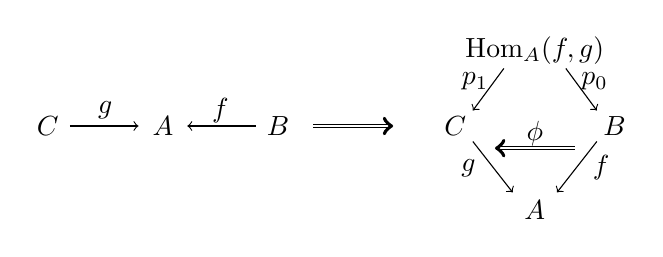
\begin{tikzpicture}[x=1.6em,y=1.6em]
  \node (C1) at (-6.8,1.0) {$C$};
  \node (A1) at (-4.2,1.0) {$A$};
  \node (B1) at (-1.6,1.0) {$B$};
  \draw[->] (-6.3,1.0) -- (-4.75,1.0);
  \node at (-5.5,1.35) {$g$};
  \draw[->] (-2.1,1.0) -- (-3.65,1.0);
  \node at (-2.9,1.35) {$f$};
  \draw[double,->] (-0.8,1.0) -- (1.0,1.0);
  \node at (4.2,2.7) {$\mathrm{Hom}_A(f,g)$};
  \node (C2) at (2.4,1.0) {$C$};
  \node (B2) at (6.0,1.0) {$B$};
  \node (A2) at (4.2,-0.9) {$A$};
  \draw[->] (3.5,2.3) -- (2.8,1.35);   %
  \node at (2.85,2.0) {$p_1$};
  \draw[->] (4.9,2.3) -- (5.6,1.35);   %
  \node at (5.55,2.0) {$p_0$};
  \draw[->] (2.8,0.65) -- (3.7,-0.5);  %
  \node at (2.7,0.05) {$g$};
  \draw[->] (5.6,0.65) -- (4.7,-0.5);  %
  \node at (5.7,0.05) {$f$};
  \draw[double,->] (5.1,0.5) -- (3.3,0.5);  %
  \node at (4.2,0.82) {$\phi$};
\end{tikzpicture}
\end{center}

本章的目标，是从一个\trInfinityCosmos{}的\trHomotopyTwoCategory{}的观点出发%
发展逗号构造的一般理论。
这项工作的第一笔收益将出现在第 4 章中，届时我们将沿这些路线研究%
\trAdjunction{}、\trLimit{}与\trColimit{}的\trUniversalProperty。逗号构造也在%
第三部分中，为确立本书通篇引入的那些\trCategory{}论概念的%
\trModelIndependence{}提供了本质性的载体。

「逗号对象」有一个标准的定义，可在任何 2-范畴中陈述，它把逗号对象定义为%
一种特定的\trWeightedLimit{}（见例 A.6.14）。
然而，\trCommaInfinityCategory{}却并\emph{不}在\trHomotopyTwoCategory{}中%
满足这个\trUniversalProperty。毋宁说，它们满足的是通常 2-范畴性%
\trUniversalProperty{}的一个颇为特别的「弱」变体——据我们所知，这一变体%
尚未在文献中别处出现过。这个弱\trUniversalProperty{}由我们称之为%
\trSmotheringFunctor{}的东西来编码，它关联起适当形状的\trHomotopy{}相干%
\trDiagram{}与\trHomotopy{}交换\trDiagram。为了在一个具体而非抽象的框架中%
引入这些\trUniversalProperty，我们从 §3.1 开始，考察涉及\trQuasiCategory{}之%
\trHomotopyCategory{}的诸\trSmotheringFunctor{}。

在 §3.2 中，我们用一个\trSmotheringFunctor{}为与一个\trInfinityCategory{} $A$%
（视作\trHomotopyTwoCategory{}中的对象）相关联的\trArrowInfinityCategory{}%
$A^{\qcTwo}$ 编码其弱\trUniversalProperty。在 §3.3 中，我们简略研究与一个%
\trIsofibration{}的\trPullback{}相关联的类似弱\trUniversalProperty，并利用%
它们证明：沿一个\trIsofibration{}对一个\trEquivalence{}取\trPullback{}，%
所得仍是\trEquivalence。

\trCommaInfinityCategory{}将在 §3.4 中引入，我们在该节中既描述它们作为%
\trSimpliciallyEnrichedLimit{}的严格\trUniversalProperty，也描述它们在%
\trHomotopyTwoCategory{}中的弱\trUniversalProperty。两者各有其用——例如%
用于描述：它们的生成\trCospan{}之间各种类型的态射在\trCommaInfinityCategory{}%
上诱导的作用。弱 2-范畴性\trUniversalProperty{}在 §3.5 中被用于证明一个%
一般的可表示性定理，该定理刻画那些被一个\trFunctor{}右表示或左表示的%
\trCommaInfinityCategory{}。在第 4 章中，我们将收获这项工作的回报：作为这些%
一般结果的特殊情形，得到对\trAdjunction{}、\trLimit{}与\trColimit{}的%
所期望的可表示刻画。

在 §3.6 中，我们把 §3.5 的主定理收紧为如下陈述：一个\trCommaInfinityCategory{}%
被一个\trFunctor{}右表示，当且仅当——把它视作\trSliceInfinityCosmos{}中的%
一个对象时——其余定义域投影函子拥有一个\trTerminal{}元素。这一结果要求对%
以下两者之间的微妙差别作仔细分析：一个\trSliceInfinityCosmos{}的%
\trHomotopyTwoCategory{}，与一个\trInfinityCosmos{}的\trHomotopyTwoCategory{}%
的切片 2-范畴。
不愿深陷草丛细节的读者，请留意定义 3.6.5 与推论 3.6.10，除此之外径直%
跳过本节即可。

\providecommand{\qcOne}{\mathbf{1}}   %
\providecommand{\qcTwo}{\mathbf{2}}   %
\providecommand{\qcInt}{\mathbb{I}}   %
\providecommand{\Cat}{\mathcal{C}at}
\providecommand{\QCat}{\mathcal{Q}\mathcal{C}at}

\section{\trSmotheringFunctor}\label{sec:smothering-functors}

设 $Q$ 是一个\trQuasiCategory{}。由引理 1.1.12 回忆起，它的\trHomotopyCategory{}%
$\mathrm{h}Q$ 具有：
\begin{itemize}
\item 对象：$Q$ 的诸\trElement{}；
\item 箭头：$Q$ 的 1-\trSimplex{}的诸\trHomotopy{}类——其中平行的 1-\trSimplex{}是%
\trHomotopic{}，当且仅当它们界定一个 2-\trSimplex{}，而其余的那条外侧边退化；以及
\item 一个合成关系——当且仅当代表这三个箭头的任意一组选定的 1-\trSimplex{}都%
界定一个 2-\trSimplex{}。
\end{itemize}
对 1-\trCategory{} $J$，经典\trHomotopy{}论中众所周知：图表的\trHomotopyCategory{}%
$\mathrm{h}(Q^J)$ 并不\trEquivalence{}于\trHomotopyCategory{}中的图表之\trCategory{}%
$(\mathrm{h}Q)^J$——除非在非常特殊的情形，比如 $J$ 是一个集合时（见引理 2.3.3）。
$\mathrm{h}(Q^J)$ 的对象是 $Q$ 中形状为 $J$ 的\emph{\trHomotopy{}相干\trDiagram}，而%
$(\mathrm{h}Q)^J$ 的对象只是\emph{\trHomotopy{}交换\trDiagram}。%
然而，存在一个典范的比较函子
\[
\mathrm{h}(Q^J)\longrightarrow(\mathrm{h}Q)^J
\]
它由把 $\mathrm{h}\colon\QCat\to\Cat$ 作用于求值函子 $Q^J\times J\to Q$ 再转置而得；
\trHomotopy{}相干\trDiagram{}特别地也是\trHomotopy{}交换\trDiagram{}。

我们在本节中的第一个目标是更好地理解\trHomotopyCategory{} $\mathrm{h}Q$ 中的箭头%
与 $Q$ 的箭头——即\trQuasiCategory{}中的 1-\trSimplex{}——之间的关系。为研究这一点，
我们考察\trQuasiCategory{} $Q^{\qcTwo}$：$Q$ 的箭头作为\trElement{}居于其中，其中%
$\qcTwo=\Delta[1]$ 是行走箭头（walking arrow）的\trNerve{}。%
我们的记号有意模仿\textbf{箭头范畴}（category of arrows）的惯用记号：若 $C$ 是%
一个 1-\trCategory{}，则 $C^{\qcTwo}$ 是这样一个\trCategory{}，其对象是 $C$ 中的%
箭头，其态射是交换方块，且视作从竖放于左侧的箭头到竖放于右侧的箭头的态射。%
这一记号上的混同引出我们的第一个问题：$Q^{\qcTwo}$ 的\trHomotopyCategory{}与%
\trHomotopyCategory{} $\mathrm{h}Q$ 中的箭头范畴之间有何关系？

\begin{lemma}\label{lem:canonical-q2}
典范函子 $\mathrm{h}(Q^{\qcTwo})\to(\mathrm{h}Q)^{\qcTwo}$：
\begin{enumerate}[label=(\roman*)]
\item 对象上满射；
\item 满；以及
\item 保守——即反射态射的可逆性，%
\end{enumerate}
但未必对象上单，也未必忠实。
\end{lemma}

\begin{proof}
对象上的满射断言：\trHomotopyCategory{} $\mathrm{h}Q$ 中的每个箭头都由 $Q$ 中的%
一个 1-\trSimplex{}所代表。这正是练习 1.1.iii(iii) 的结论，该练习概述了引理%
1.1.12 的证明。
为证满性，考察 $Q$ 中的一对箭头 $f$ 与 $g$，它们构成 $\mathrm{h}Q$ 中某个交换%
方块的源与目标。据 (i)，我们可以任取代表 $\mathrm{h}Q$ 中各态射及其公共合成的%
1-\trSimplex{}：
\begin{center}
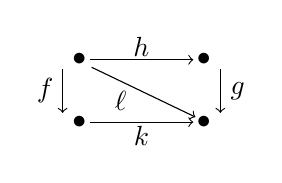
\begin{tikzpicture}[x=1.5em,y=1.5em]
  \node (tl) at (0,1.5) {$\bullet$};
  \node (tr) at (3,1.5) {$\bullet$};
  \node (bl) at (0,0) {$\bullet$};
  \node (br) at (3,0) {$\bullet$};
  \draw[->] (0.25,1.5) -- (2.75,1.5);
  \node at (1.5,1.82) {$h$};
  \draw[->] (-0.4,1.28) -- (-0.4,0.22);
  \node at (-0.82,0.75) {$f$};
  \draw[->] (3.4,1.28) -- (3.4,0.22);
  \node at (3.82,0.75) {$g$};
  \draw[->] (0.25,0) -- (2.75,0);
  \node at (1.5,-0.34) {$k$};
  \draw[->] (0.3,1.32) -- (2.8,0.12);
  \node at (1.0,0.52) {$\ell$};
\end{tikzpicture}
\end{center}
由引理 1.1.12，$\mathrm{h}Q$ 中的每个合成关系都由 $Q$ 中的一个 2-\trSimplex{}见证；%
选取一对这样的 2-\trSimplex{}便定义了一个图表 $\qcTwo\times\qcTwo\to Q$，它代表%
$\mathrm{h}(Q^{\qcTwo})$ 中一个从 $f$ 到 $g$ 的态射，满性得证。
函子 $\mathrm{h}(Q^{\qcTwo})\to(\mathrm{h}Q)^{\qcTwo}$ 的对象满射性与满性是与\trDiagram{}%
形状 $\qcTwo$ 相关的特殊性质，而保守性据推论 1.1.22 对一般的\trDiagram{}形状成立。
展示对象单性与忠实性普遍失效的反例之构造留作\cref{ex:smothering-counterexample}，%
并附有提示。
\end{proof}

典范函子 $\mathrm{h}(Q^{\qcTwo})\to(\mathrm{h}Q)^{\qcTwo}$ 的这些性质将反复出现，
故我们以一个发人联想的名字为它们命名：

\begin{definition}[\trSmotheringFunctor]\label{def:smothering-functor}
1-\trCategory{}之间的\trFunctor{} $f\colon A\to B$ 是\textbf{\trSmothering}（smothering），%
若它在对象上满射、满且保守。也就是说，一个\trFunctor{}是\trSmothering{}，当且仅当它对%
下列\trFunctor{}之集具有右提升性质：
\[
\left\{\;
\mbox{\begin{tikzpicture}[x=1.2em,y=1.2em]
  \node (a) at (0,0.9) {$\varnothing$};
  \node (b) at (0,-0.9) {$\qcOne$};
  \draw[->] (0,0.5) -- (0,-0.5);
  \draw (0,0.5) arc[start angle=180,end angle=0,radius=0.15];
\end{tikzpicture}}
\;,\;
\mbox{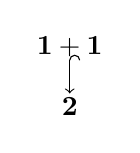
\begin{tikzpicture}[x=1.2em,y=1.2em]
  \node (a) at (0,0.9) {$\qcOne+\qcOne$};
  \node (b) at (0,-0.9) {$\qcTwo$};
  \draw[->] (0,0.5) -- (0,-0.5);
  \draw (0,0.5) arc[start angle=180,end angle=0,radius=0.15];
\end{tikzpicture}}
\;,\;
\mbox{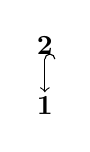
\begin{tikzpicture}[x=1.2em,y=1.2em]
  \node (a) at (0,0.9) {$\qcTwo$};
  \node (b) at (0,-0.9) {$\qcOne$};
  \draw[->] (0,0.5) -- (0,-0.5);
  \draw (0,0.5) arc[start angle=180,end angle=0,radius=0.15];
\end{tikzpicture}}
\;\right\}
\]
\end{definition}

\cref{ex:smothering-properties}建立了覆盖函子的诸多初等性质；这里我们强调其中%
一条值得特别留意的：

\begin{lemma}[\trSmotheringFunctor{}的\trFiber]\label{lem:smothering-fibers}
覆盖函子的每条\trFiber{}都是非空连通\trGroupoid{}。
\end{lemma}

\begin{proof}
设 $f\colon A\to B$ 是\trSmothering{}，考察 $B$ 中对象 $b$ 上的\trFiber{}：
\begin{center}
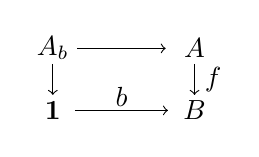
\begin{tikzpicture}[x=1.6em,y=1.6em]
  \node (tl) at (0,1.4) {$A_b$};
  \node (tr) at (3.2,1.4) {$A$};
  \node (bl) at (0,0) {$\qcOne$};
  \node (br) at (3.2,0) {$B$};
  \draw[->] (0.55,1.4) -- (2.55,1.4);
  \draw[->] (0,1.05) -- (0,0.35);
  \node at (0.45,0.78) {$\scriptstyle\lrcorner$};
  \draw[->] (3.2,1.05) -- (3.2,0.35);
  \node at (3.62,0.7) {$f$};
  \draw[->] (0.5,0) -- (2.6,0);
  \node at (1.55,0.3) {$b$};
\end{tikzpicture}
\end{center}
由对象上的满射性，\trFiber{}非空。\trFiber{}中的态射定义为 $b$ 的\trFiber{}中对象之间、且映到%
$b$ 上恒同的箭头。由满性，\trFiber{}中的任意两个对象都由一个态射相连，甚至由指向%
两个方向的态射相连。由保守性，\trFiber{}中的所有态射都必然是\trInvertible{}。
\end{proof}

用于证明\cref{lem:canonical-q2}的论证可推广为：

\begin{lemma}\label{lem:smothering-free}
若 $J$ 是一个在\trReflexiveDirectedGraph{}上\trFree 1-\trCategory{}，而 $Q$ 是一个%
\trQuasiCategory{}，则典范函子 $\mathrm{h}(Q^J)\to(\mathrm{h}Q)^J$ 是\trSmothering{}。
\end{lemma}
\begin{proof}
见\cref{ex:smothering-free}。
\end{proof}

\trCotensor{}是定义 1.2.1 所公理化的诸\trCosmologicalLimitNotions{}之一。
那里列出的其他\trLimit{}构造也给出覆盖函子。

\begin{lemma}\label{lem:smothering-pullback}
对由\trQuasiCategory{}构成的任何\trPullback{}图表，其中 $p$ 是\trIsofibration{}：
\begin{center}
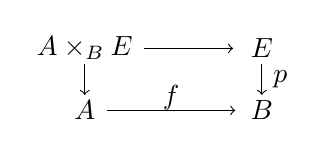
\begin{tikzpicture}[x=1.6em,y=1.6em]
  \node (tl) at (0,1.4) {$A\times_BE$};
  \node (tr) at (4.0,1.4) {$E$};
  \node (bl) at (0,0) {$A$};
  \node (br) at (4.0,0) {$B$};
  \draw[->] (1.35,1.4) -- (3.35,1.4);
  \draw[->] (0,1.05) -- (0,0.35);
  \node at (0.45,0.78) {$\scriptstyle\lrcorner$};
  \draw[->] (4.0,1.05) -- (4.0,0.35);
  \node at (4.42,0.7) {$p$};
  \draw[->] (0.5,0) -- (3.4,0);
  \node at (1.95,0.3) {$f$};
\end{tikzpicture}
\end{center}
典范函子 $\mathrm{h}(A\times_BE)\to\mathrm{h}A\times_{\mathrm{h}B}\mathrm{h}E$ 是\trSmothering{}。
\end{lemma}
\begin{proof}
由于 $\mathrm{h}\colon\QCat\to\Cat$ 不保持\trPullback{}，题中的典范比较函子不是%
\trIsomorphism{}。但它对象上双射，因为复合函子
\[
\QCat\xrightarrow{\;\mathrm{h}\;}\Cat\xrightarrow{\;\mathrm{obj}\;}\mathcal{S}et
\]
落到每个\trQuasiCategory{}的底层顶点集上，且该函子\emph{确实}保持\trPullback{}。

为证满性，注意 $\mathrm{h}A\times_{\mathrm{h}B}\mathrm{h}E$ 中的态射由一对%
1-\trSimplex{}代表——$A$ 中的 $\alpha\colon a\to a'$ 与 $E$ 中的%
$\epsilon\colon e\to e'$，它们的像在 $B$ 中\trHomotopic——这一条件特别地蕴含%
$f(a)=p(e)$ 与 $f(a')=p(e')$。

由引理 1.1.9，我们可以随心所欲地配置这一\trHomotopy{}，于是选取 2-\trSimplex{}%
见证者 $\beta$，以定义如下的\trLifting{}问题
\begin{center}
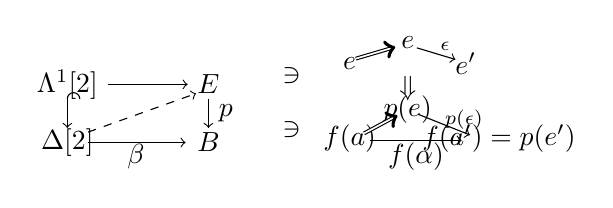
\begin{tikzpicture}[x=1.5em,y=1.5em]
  \node (tl) at (0,1.4) {$\Lambda^1[2]$};
  \node (tr) at (3.4,1.4) {$E$};
  \node (bl) at (0,0) {$\Delta[2]$};
  \node (br) at (3.4,0) {$B$};
  \draw[->] (tl) -- (tr);
  \draw[->] (0,1.05) -- (0,0.35);
  \draw (0,1.05) arc[start angle=180,end angle=0,radius=0.15];
  \draw[->] (3.4,1.05) -- (3.4,0.35);
  \node at (3.82,0.7) {$p$};
  \draw[->] (0.5,0) -- (2.85,0);
  \node at (1.65,-0.35) {$\beta$};
  \draw[->,dashed] (0.5,0.25) -- (3.1,1.18);
  \node at (5.4,1.6) {$\ni$};
  \node (e0) at (6.8,1.9) {$e$};
  \node (e1) at (8.2,2.4) {$e$};
  \node (e2) at (9.6,1.9) {$e'$};
  \draw[double,->] (6.95,2.02) -- (7.9,2.3);
  \draw[->] (8.42,2.28) -- (9.35,2.0);
  \node at (9.1,2.32) {$\scriptstyle\epsilon$};
  \node at (8.2,1.3) {$\Downarrow$};
  \node at (5.4,0.3) {$\ni$};
  \node (fa) at (6.8,0.1) {$f(a)$};
  \node (pe) at (8.2,0.8) {$p(e)$};
  \node (fp) at (10.4,0.1) {$f(a')=p(e')$};
  \draw[double,->] (7.15,0.22) -- (7.95,0.65);
  \draw[->] (8.45,0.68) -- (9.7,0.18);
  \node at (9.55,0.55) {$\scriptstyle p(\epsilon)$};
  \draw[->] (7.3,0.05) -- (9.5,0.05);
  \node at (8.4,-0.35) {$f(\alpha)$};
\end{tikzpicture}
\end{center}
由于 $p$ 是\trIsofibration{}，解存在，它定义了 $E$ 中与 $\epsilon$ 属同一%
\trHomotopy{}类的一条箭头 $\tilde{\epsilon}\colon e\to e'$，使得%
$p(\tilde{\epsilon})=f(\alpha)$。数对 $(\alpha,\tilde{\epsilon})$ 现在便定义了%
$\mathrm{h}(E\times_BA)$ 中所提升的那条箭头。

最后，考虑一条箭头 $\qcTwo\to A\times_BE$，它在 $\mathrm{h}A\times_{\mathrm{h}B}\mathrm{h}E$ 中的像是\trIsomorphism——这只在到 $E$ 与到 $A$ 的投影都定义%
\trIsomorphism{}时发生。由推论 1.1.16，我们可以选取一个%
\trHomotopyCoherentIsomorphism{} $\qcInt\to A$，扩张给定的\trIsomorphism{}%
$\qcTwo\to A$。这份数据向我们呈现如下\trLifting{}问题
\begin{center}
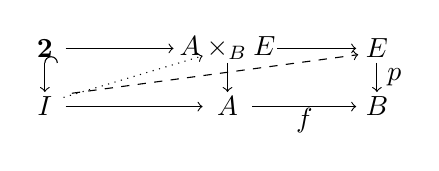
\begin{tikzpicture}[x=1.5em,y=1.5em]
  \node (tl) at (0,1.4) {$\qcTwo$};
  \node (tm) at (4.4,1.4) {$A\times_BE$};
  \node (tr) at (8.0,1.4) {$E$};
  \node (bl) at (0,0) {$\qcInt$};
  \node (bm) at (4.4,0) {$A$};
  \node (br) at (8.0,0) {$B$};
  \draw[->] (0.5,1.4) -- (3.1,1.4);
  \draw[->] (5.6,1.4) -- (7.5,1.4);
  \draw[->] (0,1.05) -- (0,0.35);
  \draw (0,1.05) arc[start angle=180,end angle=0,radius=0.15];
  \draw[->] (4.4,1.05) -- (4.4,0.35);
  \node at (4.85,0.82) {$\scriptstyle\lrcorner$};
  \draw[->] (8.0,1.05) -- (8.0,0.35);
  \node at (8.42,0.7) {$p$};
  \draw[->] (0.5,0) -- (3.8,0);
  \draw[->] (5.0,0) -- (7.5,0);
  \node at (6.25,-0.35) {$f$};
  \draw[->,dotted] (0.45,0.22) -- (3.8,1.22);
  \draw[->,dashed] (0.65,0.32) -- (7.55,1.25);
\end{tikzpicture}
\end{center}
而练习 1.1.vi 告诉我们它可以求解。
这便证明了 $\mathrm{h}(A\times_BE)\to\mathrm{h}A\times_{\mathrm{h}B}\mathrm{h}E$ 是%
\trConservative{}，从而也是\trSmothering{}。
\end{proof}

类似的论证可证明：

\begin{lemma}\label{lem:smothering-tower}
对\trQuasiCategory{}之间的任何\trIsofibration{}之塔
\[
\cdots\twoheadrightarrow E_n\twoheadrightarrow E_{n-1}\twoheadrightarrow\cdots
\twoheadrightarrow E_2\twoheadrightarrow E_1\twoheadrightarrow E_0
\]
典范函子 $\mathrm{h}(\lim_n E_n)\to\lim_n\mathrm{h}E_n$ 是\trSmothering{}。
\end{lemma}
\begin{proof}
见\cref{ex:smothering-tower}。
\end{proof}

\begin{lemma}\label{lem:smothering-hom}
对\trQuasiCategory{}之间的任何余跨度 $C\xrightarrow{\;g\;}A\xleftarrow{\;f\;}B$，
考察由如下\trPullback{}定义的\trQuasiCategory
\begin{center}
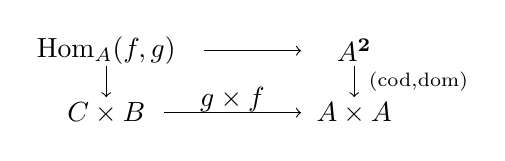
\begin{tikzpicture}[x=1.6em,y=1.6em]
  \node (tl) at (0,1.4) {$\mathrm{Hom}_A(f,g)$};
  \node (tr) at (5.6,1.4) {$A^{\qcTwo}$};
  \node (bl) at (0,0) {$C\times B$};
  \node (br) at (5.6,0) {$A\times A$};
  \draw[->] (2.2,1.4) -- (4.4,1.4);
  \draw[->] (0,1.05) -- (0,0.35);
  \node at (0.45,0.78) {$\scriptstyle\lrcorner$};
  \draw[->] (5.6,1.05) -- (5.6,0.35);
  \node at (7.05,0.7) {$\scriptstyle(\mathrm{cod},\mathrm{dom})$};
  \draw[->] (1.3,0) -- (4.4,0);
  \node at (2.85,0.3) {$g\times f$};
\end{tikzpicture}
\end{center}
典范函子 $\mathrm{h}\mathrm{Hom}_A(f,g)\to\mathrm{Hom}_{\mathrm{h}A}(\mathrm{h}f,\mathrm{h}g)$%
是\trSmothering{}。
\end{lemma}

\begin{proof}
该函子的余域是由 $\Cat$ 中一个类似的\trPullback{}所定义的\trCategory
\begin{center}
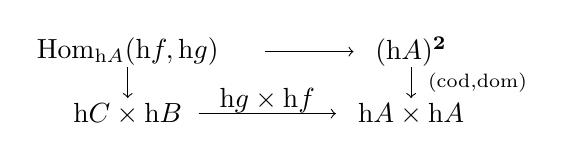
\begin{tikzpicture}[x=1.6em,y=1.6em]
  \node (tl) at (0,1.4) {$\mathrm{Hom}_{\mathrm{h}A}(\mathrm{h}f,\mathrm{h}g)$};
  \node (tr) at (6.4,1.4) {$(\mathrm{h}A)^{\qcTwo}$};
  \node (bl) at (0,0) {$\mathrm{h}C\times\mathrm{h}B$};
  \node (br) at (6.4,0) {$\mathrm{h}A\times\mathrm{h}A$};
  \draw[->] (3.1,1.4) -- (5.1,1.4);
  \draw[->] (0,1.05) -- (0,0.35);
  \node at (0.45,0.78) {$\scriptstyle\lrcorner$};
  \draw[->] (6.4,1.05) -- (6.4,0.35);
  \node at (7.9,0.7) {$\scriptstyle(\mathrm{cod},\mathrm{dom})$};
  \draw[->] (1.6,0) -- (4.7,0);
  \node at (3.15,0.3) {$\mathrm{h}g\times\mathrm{h}f$};
\end{tikzpicture}
\end{center}
而该典范函子分解为
\[
\mathrm{h}\mathrm{Hom}_{A}(f,g)\longrightarrow
\mathrm{h}(A^{\qcTwo})\times_{\mathrm{h}A\times\mathrm{h}A}(\mathrm{h}C\times\mathrm{h}B)
\longrightarrow
(\mathrm{h}A)^{\qcTwo}\times_{\mathrm{h}A\times\mathrm{h}A}(\mathrm{h}C\times\mathrm{h}B)
\]
由\cref{lem:smothering-pullback}，这些函子中的第一个是\trSmothering{}。由%
\cref{lem:canonical-q2}，第二个是某个覆盖函子的\trPullback{}。于是据%
\cref{ex:smothering-properties}(i)可得：复合函子是\trSmothering{}。
\end{proof}

在接下来的几节中，我们将发现：刚刚构造的这些覆盖函子表达了任何%
\trInfinityCosmos{}的\trHomotopyTwoCategory{}中箭头、\trPullback{}与逗号构造的%
弱\trUniversalProperty{}。

\subsection*{练习}

\begin{exercise}\label{ex:smothering-counterexample}
找一个显式的例子：一个\trQuasiCategory{} $Q$，使得典范覆盖函子%
$\mathrm{h}(Q^{\qcTwo})\to(\mathrm{h}Q)^{\qcTwo}$ 在对象上不单、也不忠实——%
例如取 $Q$ 为某个适当拓扑空间的总奇异复形。
\end{exercise}

\begin{exercise}\label{ex:smothering-properties}
证明：
\begin{enumerate}[label=(\roman*)]
\item 覆盖函子在复合、\trRetract{}、\trProduct{}、\trPullback{}与塔的\trLimit{}下封闭。
\item \trCategory{}之间的\trSurjectiveEquivalence{}是覆盖函子。
\item 覆盖函子是\trIsofibration{}，也就是说，是对 $\qcOne\hookrightarrow\qcInt$ 具有%
右提升性质的映射。
\item 证明：若 $f$ 与 $gf$ 是覆盖函子，则 $g$ 是覆盖函子。\footnote{事实上，%
只需假设 $f$ 在对象与箭头上满射便已足够。}
\end{enumerate}
\end{exercise}

\begin{exercise}\label{ex:smothering-free}
证明\cref{lem:smothering-free}。
\end{exercise}

\begin{exercise}\label{ex:smothering-tower}
证明\cref{lem:smothering-tower}。
\end{exercise}
   %
\providecommand{\qcOne}{\mathbf{1}}   %
\providecommand{\qcTwo}{\mathbf{2}}   %
\providecommand{\qcor}[1]{\ulcorner#1\urcorner}   %

\section{箭头\trInfinityCategory}\label{sec:infinity-categories-of-arrows}

本节中，我们把 3.1 节开头的讨论复刻一遍，用任意的\trInfinityCategory{} $A$ 顶替%
\trQuasiCategory{} $Q$。上一节的分析本可以在这一般性的设定中直接展开，只是代价是%
多出一层抽象与更使人混淆的记号——此时\trFunctorSpace{} $\mathrm{Fun}(X,A)$ 取代了%
\trQuasiCategory{} $Q$。
回忆：\trInfinityCategory{}的\trElement{}定义为\trFunctor{} $a\colon\qcOne\to A$。%
同义反复地说，$A$ 的诸\trElement{}正是 $A$ 的\trUnderlyingQuasiCategory{}%
$\mathrm{Fun}(\qcOne,A)$ 的诸顶点。本节中，我们定义并研究一个\trInfinityCategory{}%
$A^{2}$，其\trElement{}恰是 $A$ 的\trUnderlyingQuasiCategory{}中的诸 1-\trSimplex{}。%
我们把 $A^{2}$ 称为 $A$ 中的\textbf{\trArrowInfinityCategory}（∞-category of arrows），并径称其%
\trElement{}为 $A$ 的\emph{箭头}（arrow）。%
事实上，这一构造我们此前早已默认引入过。回忆：$\qcTwo$ 是我们对\trQuasiCategory{}%
$\Delta[1]$ 的惯用记号，它即\trCategory{} $2$——带唯一一条非恒同态射 $0\to 1$ 的%
那个——的\trNerve{}。

\begin{definition}[\trArrowInfinityCategory]\label{def:arrow-infinity-category}
设 $A$ 为一个\trInfinityCategory。$A$ 中的\trArrowInfinityCategory{}是单纯\trCotensor{}
$A^{\qcTwo}$ 连同由包含 $\partial\Delta[1]\hookrightarrow\Delta[1]$ 诱导的典范%
\trEndpointEvaluation{}等价纤维化
\[
A^{\qcTwo}\coloneqq A^{\Delta[1]}\xrightarrow[\ (p_{1},p_{0})\ ]{A^{\partial\Delta[1]}\cong A\times A}
\]
为简洁起见，我们把由包含 $0\colon\qcOne\hookrightarrow\qcTwo$ 诱导的%
\trDomainEvaluation{}记作 $p_{0}\colon A^{\qcTwo}\twoheadrightarrow A$，
把由 $1\colon\qcOne\hookrightarrow\qcTwo$ 诱导的\trCodomainEvaluation{}记作%
$p_{1}\colon A^{\qcTwo}\twoheadrightarrow A$。
\end{definition}

作为\trHomotopyTwoCategory{}中的一个对象，\trArrowInfinityCategory{}配备有一个典范 2-\trCell{}，%
我们现在就来构造它。

\begin{lemma}[\trGenericArrow]\label{lem:generic-arrow}
对任意\trInfinityCategory{} $A$，\trArrowInfinityCategory $A^{2}$ 配备有一个典范 2-\trCell
\begin{rveq}\label{eq:generic-arrow}
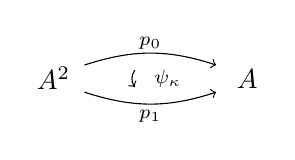
\begin{tikzpicture}[x=1.4em,y=1.4em,baseline=(current bounding box.center)]
  \node (a) at (0,0) {$A^{2}$};
  \node (b) at (5,0) {$A$};
  \draw[->] (0.8,0.35) to[bend left=18] (4.2,0.35);
  \node at (2.5,0.92) {$\scriptstyle p_{0}$};
  \draw[->] (0.8,-0.35) to[bend right=18] (4.2,-0.35);
  \node at (2.5,-0.97) {$\scriptstyle p_{1}$};
  \draw[->] (2.1,0.22) to[bend right=35] (2.1,-0.22);
  \node at (2.95,0.0) {$\scriptstyle\psi_{\kappa}$};
\end{tikzpicture}
\end{rveq}
我们称之为以 $A$ 为余定义域的\textbf{\trGenericArrow}（generic arrow）。
\end{lemma}

\begin{proof}
\trSimplicial\trCotensor{}具有题外话 1.2.6 所描述的严格\trUniversalProperty{}：%
也就是说，$A^{2}$ 由自然同构
\begin{rveq}\label{eq:fun-cotensor-iso}
\mathrm{Fun}(X,A^{2})\cong\mathrm{Fun}(X,A)^{2}
\end{rveq}
所刻画。由\trYonedaLemma{}，自然同构 \eqref{eq:fun-cotensor-iso} 的数据被其%
「\trGenericElement」所编码——后者定义为恒同在表示对象处的像。%
这里，恒同函子 $\mathrm{id}\colon A^{2}\to A^{2}$ 被映为 $\mathrm{Fun}(A^{2},A)^{2}$%
的一个\trElement——亦即 $\mathrm{Fun}(A^{2},A)$ 中的一个 1-\trSimplex——由引理%
1.4.3，它表示\trHomotopyTwoCategory{}中的一个 2-\trCell{} $\kappa$。
要看清 $\kappa$ 的源与靶必是\trDomainEvaluation{}与\trCodomainEvaluation{}这两个函子——二者由对端点%
包含 $\qcOne+\qcOne\hookrightarrow\qcTwo$ 作余张量而定义——
我们利用自然同构 \eqref{eq:fun-cotensor-iso} 在余张量变元上的自然性：
\begin{center}
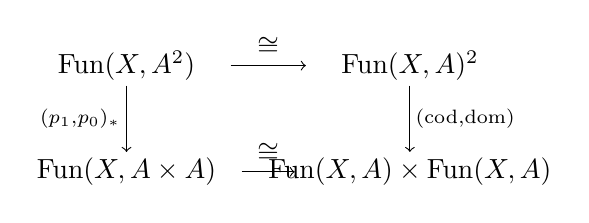
\begin{tikzpicture}[x=1.6em,y=1.6em]
  \node (tl) at (0,1.2) {$\mathrm{Fun}(X,A^{2})$};
  \node (tr) at (6.4,1.2) {$\mathrm{Fun}(X,A)^{2}$};
  \node (bl) at (0,-1.2) {$\mathrm{Fun}(X,A\times A)$};
  \node (br) at (6.4,-1.2) {$\mathrm{Fun}(X,A)\times\mathrm{Fun}(X,A)$};
  \draw[->] (2.35,1.2) -- node[above]{$\cong$} (4.05,1.2);
  \draw[->] (2.6,-1.2) -- node[above]{$\cong$} (3.8,-1.2);
  \draw[->] (0,0.75) -- (0,-0.75);
  \node at (-1.05,0) {$\scriptstyle(p_{1},p_{0})_{*}$};
  \draw[->] (6.4,0.75) -- (6.4,-0.75);
  \node at (7.65,0) {$\scriptstyle(\mathrm{cod},\mathrm{dom})$};
\end{tikzpicture}
\end{center}
恒同函子沿右上复合被映到函子对 $(\mathrm{cod}\,\kappa,\mathrm{dom}\,\kappa)$，而沿%
左下复合被映到函子对 $(p_{1},p_{0})$。
\end{proof}

存在一个与\cref{def:arrow-infinity-category}相类比的 2-范畴论\trLimit{}概念：它对%
任意对象 $A$ 构造以 $A$ 为余定义域的泛 2-\trCell——亦即与 1-\trCategory{} $2$ 作的%
（范畴论的）\trCotensor{}。其\trUniversalProperty{}与 \eqref{eq:fun-cotensor-iso}%
相类似，只是以该 2-\trCategory{}的 \trHomCategory{}顶替\trFunctorSpace{}（见定义 A.4.1）。%
在\trCategory{}的 2-\trCategory{}中，2-\trCotensor{}定义了\trCategoryOfArrows{}。
在\trHomotopyTwoCategory{}中，再次由\trYonedaLemma{}，数据 \eqref{eq:generic-arrow}%
编码了\trCategory{}之间的一个\trNaturalTransformation
\[
\mathrm{hFun}(X,A^{2})\longrightarrow\mathrm{hFun}(X,A)^{2}
\]
但它并\emph{不是}自然同构，甚至连\trCategory{}之间的自然等价也不是。不过，它确实%
赋予\trArrowInfinityCategory{}一条如下形式的「弱」\trUniversalProperty{}：

\begin{proposition}[\trArrowInfinityCategory{}的弱泛性质]\label{prop:weak-universal-property}
以 $A$ 为余定义域的\trGenericArrow \eqref{eq:generic-arrow} 在\trHomotopyTwoCategory{}中%
具有由下述三种运算给出的弱\trUniversalProperty{}：
\begin{enumerate}[label=(\roman*)]
\item \textbf{1-\trCell{}归纳：}%
给定 $A$ 上的一项\trNaturalTransformation{}，如下左图所示：
\begin{center}
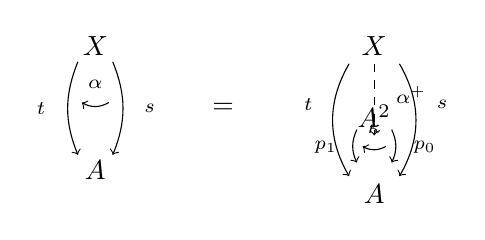
\begin{tikzpicture}[x=1.4em,y=1.4em]
  \node (Xl) at (0,1.6) {$X$};
  \node (Al) at (0,-1.6) {$A$};
  \draw[->] (-0.45,1.2) to[bend right=22] (-0.45,-1.2);
  \node at (-1.4,0) {$\scriptstyle t$};
  \draw[->] (0.45,1.2) to[bend left=22] (0.45,-1.2);
  \node at (1.4,0) {$\scriptstyle s$};
  \draw[->] (0.35,0.15) to[bend left=30] (-0.35,0.15);
  \node at (0,0.62) {$\scriptstyle\alpha$};
  \node at (3.3,0) {$=$};
  \node (Xr) at (7.2,1.6) {$X$};
  \node (M) at (7.2,-0.2) {$A^{2}$};
  \node (Ar) at (7.2,-2.2) {$A$};
  \draw[->,dashed] (7.2,1.15) -- (7.2,-0.7);
  \node at (8.15,0.35) {$\scriptstyle\ulcorner\alpha^{+}\urcorner$};
  \draw[->] (6.55,1.15) to[bend right=30] (6.55,-1.75);
  \node at (5.5,0.1) {$\scriptstyle t$};
  \draw[->] (7.85,1.15) to[bend left=30] (7.85,-1.75);
  \node at (8.95,0.1) {$\scriptstyle s$};
  \draw[->] (6.75,-0.55) to[bend right=25] (6.75,-1.4);
  \node at (5.95,-1.0) {$\scriptstyle p_{1}$};
  \draw[->] (7.65,-0.55) to[bend left=25] (7.65,-1.4);
  \node at (8.5,-1.0) {$\scriptstyle p_{0}$};
  \draw[->] (7.5,-0.98) to[bend left=30] (6.9,-0.98);
  \node at (7.2,-0.55) {$\scriptstyle\kappa$};
\end{tikzpicture}
\end{center}
则存在\trFunctor{} $\qcor{\alpha^{+}}\colon X\to A^{2}$，使得 $s=p_{0}\qcor{\alpha^{+}}$、%
$t=p_{1}\qcor{\alpha^{+}}$，且 $\alpha=\kappa\qcor{\alpha^{+}}$。
\item \textbf{2-\trCell{}归纳：}%
给定\trFunctor{} $a,a'\colon X\to A^{2}$ 与\trNaturalTransformation{} $\tau_{1}$、%
$\tau_{0}$，使得
\begin{center}
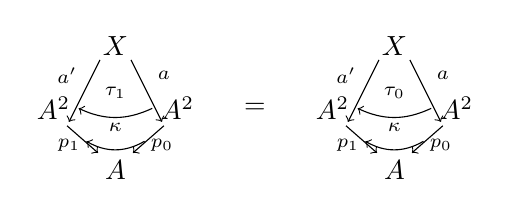
\begin{tikzpicture}[x=1.4em,y=1.4em]
  \node (X) at (0,1.5) {$X$};
  \node (Ml) at (-1.6,-0.1) {$A^{2}$};
  \node (Mr) at (1.6,-0.1) {$A^{2}$};
  \node (A) at (0,-1.7) {$A$};
  \draw[->] (-0.4,1.15) -- (-1.2,-0.45);
  \node at (-1.25,0.75) {$\scriptstyle a'$};
  \draw[->] (0.4,1.15) -- (1.2,-0.45);
  \node at (1.25,0.75) {$\scriptstyle a$};
  \draw[->] (0.95,-0.1) to[bend left=25] (-0.95,-0.1);
  \node at (0,0.3) {$\scriptstyle\tau_{1}$};
  \draw[->] (-1.25,-0.55) -- (-0.45,-1.25);
  \node at (-1.2,-1.05) {$\scriptstyle p_{1}$};
  \draw[->] (1.25,-0.55) -- (0.45,-1.25);
  \node at (1.2,-1.05) {$\scriptstyle p_{0}$};
  \draw[->] (0.75,-0.95) to[bend left=30] (-0.75,-0.95);
  \node at (0,-0.58) {$\scriptstyle\kappa$};
  \node at (3.6,-0.1) {$=$};
  \begin{scope}[shift={(7.2,0)}]
  \node (X) at (0,1.5) {$X$};
  \node (Ml) at (-1.6,-0.1) {$A^{2}$};
  \node (Mr) at (1.6,-0.1) {$A^{2}$};
  \node (A) at (0,-1.7) {$A$};
  \draw[->] (-0.4,1.15) -- (-1.2,-0.45);
  \node at (-1.25,0.75) {$\scriptstyle a'$};
  \draw[->] (0.4,1.15) -- (1.2,-0.45);
  \node at (1.25,0.75) {$\scriptstyle a$};
  \draw[->] (0.95,-0.1) to[bend left=25] (-0.95,-0.1);
  \node at (0,0.3) {$\scriptstyle\tau_{0}$};
  \draw[->] (-1.25,-0.55) -- (-0.45,-1.25);
  \node at (-1.2,-1.05) {$\scriptstyle p_{1}$};
  \draw[->] (1.25,-0.55) -- (0.45,-1.25);
  \node at (1.2,-1.05) {$\scriptstyle p_{0}$};
  \draw[->] (0.75,-0.95) to[bend left=30] (-0.75,-0.95);
  \node at (0,-0.58) {$\scriptstyle\kappa$};
  \end{scope}
\end{tikzpicture}
\end{center}
则存在\trNaturalTransformation{} $\tau\colon a\Rightarrow a'$，使得 $p_{1}\tau=\tau_{1}$%
且 $p_{0}\tau=\tau_{0}$。
\item \textbf{2-\trCell{}保守性：}%
对任何\trNaturalTransformation
\begin{center}
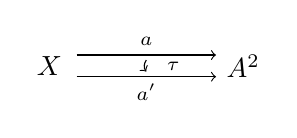
\begin{tikzpicture}[x=1.4em,y=1.4em]
  \node (X) at (0,0) {$X$};
  \node (M) at (5,0) {$A^{2}$};
  \draw[->] (0.7,0.28) -- (4.3,0.28);
  \node at (2.5,0.64) {$\scriptstyle a$};
  \draw[->] (0.7,-0.28) -- (4.3,-0.28);
  \node at (2.5,-0.68) {$\scriptstyle a'$};
  \draw[->] (2.5,0.15) to[bend right=35] (2.5,-0.15);
  \node at (3.2,0.0) {$\scriptstyle\tau$};
\end{tikzpicture}
\end{center}
若 $p_{1}\tau$ 与 $p_{0}\tau$ 皆为\trIsomorphism{}，则 $\tau$ 是\trIsomorphism{}。
\end{enumerate}
\end{proposition}

\begin{proof}
令 $Q=\mathrm{Fun}(X,A)$ 并应用引理 3.1.1，可见 \trHomCategory{}之间的自然映射
\begin{center}
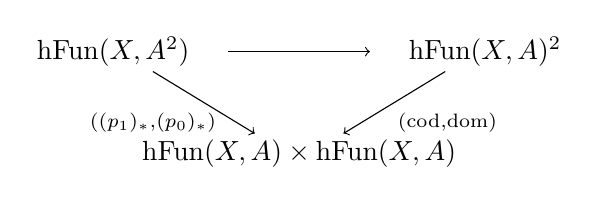
\begin{tikzpicture}[x=1.6em,y=1.6em]
  \node (tl) at (0,1.3) {$\mathrm{hFun}(X,A^{2})$};
  \node (tr) at (8.4,1.3) {$\mathrm{hFun}(X,A)^{2}$};
  \node (bm) at (4.2,-1.0) {$\mathrm{hFun}(X,A)\times\mathrm{hFun}(X,A)$};
  \draw[->] (2.6,1.3) -- (5.8,1.3);
  \draw[->] (0.9,0.85) -- (3.2,-0.55);
  \node at (0.9,-0.3) {$\scriptstyle((p_{1})_{*},(p_{0})_{*})$};
  \draw[->] (7.5,0.85) -- (5.2,-0.55);
  \node at (7.55,-0.3) {$\scriptstyle(\mathrm{cod},\mathrm{dom})$};
\end{tikzpicture}
\end{center}
——它居于 $\mathrm{hFun}(X,A\times A)\cong\mathrm{hFun}(X,A)\times\mathrm{hFun}(X,A)$%
之上——是一个\trSmotheringFunctor{}。对象上的满射性由 1-\trCell{}归纳表达，满性由%
2-\trCell{}归纳表达，而保守性由 2-\trCell{}保守性表达。
\end{proof}

注意，表示一个给定的\trNaturalTransformation{} $\alpha$（以 $X$ 为定义域、以 $A$ 为%
余定义域）的诸\trFunctor{} $\qcor{\alpha^{+}}\colon X\to A^{2}$ 并不唯一。然而，它们在%
「纤维化」同构之下唯一——这类同构与 $(p_{1},p_{0})\colon A^{2}\twoheadrightarrow A\times A$%
作\trWhiskering{}后成为恒同：%

\begin{proposition}\label{prop:whiskering-bijection}
与 \eqref{eq:generic-arrow} 的\trWhiskering{}在如下左所示的、以 $X$ 为定义域且以 $A$ 为%
余定义域的诸\trNaturalTransformation{}，与如下右所示的、诸\trFunctor{} $X\to A^{2}$ 的%
\trFiberedIsomorphism{}类之间诱导出一个双射：
\[
\left\{\vcenter{\hbox{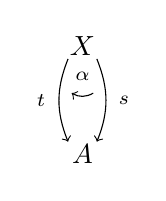
\begin{tikzpicture}[x=1.3em,y=1.3em]
  \node (X) at (0,1.5) {$X$};
  \node (A) at (0,-1.5) {$A$};
  \draw[->] (-0.4,1.15) to[bend right=22] (-0.4,-1.15);
  \node at (-1.15,0) {$\scriptstyle t$};
  \draw[->] (0.4,1.15) to[bend left=22] (0.4,-1.15);
  \node at (1.15,0) {$\scriptstyle s$};
  \draw[->] (0.3,0.2) to[bend left=30] (-0.3,0.2);
  \node at (0,0.66) {$\scriptstyle\alpha$};
\end{tikzpicture}}}\right\}
\;\longleftrightarrow\;
\left\{\vcenter{\hbox{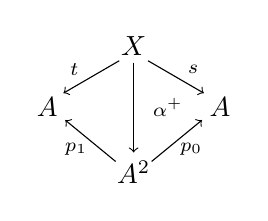
\begin{tikzpicture}[x=1.3em,y=1.3em]
  \node (X) at (0,1.6) {$X$};
  \node (Al) at (-2.4,-0.1) {$A$};
  \node (Ar) at (2.4,-0.1) {$A$};
  \node (M) at (0,-1.9) {$A^{2}$};
  \draw[->] (-0.4,1.2) -- (-1.95,0.3);
  \node at (-1.65,0.95) {$\scriptstyle t$};
  \draw[->] (0.4,1.2) -- (1.95,0.3);
  \node at (1.65,0.95) {$\scriptstyle s$};
  \draw[->] (0,1.15) -- (0,-1.35);
  \node at (0.95,-0.1) {$\scriptstyle\ulcorner\alpha^{+}\urcorner$};
  \draw[->] (-0.5,-1.6) -- (-1.9,-0.45);
  \node at (-1.6,-1.25) {$\scriptstyle p_{1}$};
  \draw[->] (0.5,-1.6) -- (1.9,-0.45);
  \node at (1.6,-1.25) {$\scriptstyle p_{0}$};
\end{tikzpicture}}}\right\}_{/\cong}
\]
其中诸\trFiberedIsomorphism{}由可逆 2-\trCell
\begin{center}
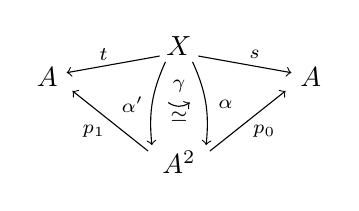
\begin{tikzpicture}[x=1.4em,y=1.4em]
  \node (X) at (0,1.7) {$X$};
  \node (Al) at (-3.4,0.9) {$A$};
  \node (Ar) at (3.4,0.9) {$A$};
  \node (M) at (0,-1.3) {$A^{2}$};
  \draw[->] (-0.5,1.45) -- (-2.9,1.02);
  \node at (-1.95,1.5) {$\scriptstyle t$};
  \draw[->] (0.5,1.45) -- (2.9,1.02);
  \node at (1.95,1.5) {$\scriptstyle s$};
  \draw[->] (-0.35,1.3) to[bend right=15] (-0.7,-0.85);
  \node at (-1.2,0.2) {$\scriptstyle\ulcorner\alpha'\urcorner$};
  \draw[->] (0.35,1.3) to[bend left=15] (0.7,-0.85);
  \node at (1.2,0.2) {$\scriptstyle\ulcorner\alpha\urcorner$};
  \draw[->] (-0.28,0.25) to[bend right=35] (0.28,0.25);
  \node at (0,0.68) {$\scriptstyle\gamma$};
  \node at (0,-0.12) {$\scriptstyle\simeq$};
  \draw[->] (-0.8,-1.0) -- (-2.75,0.55);
  \node at (-2.2,-0.5) {$\scriptstyle p_{1}$};
  \draw[->] (0.8,-1.0) -- (2.75,0.55);
  \node at (2.2,-0.5) {$\scriptstyle p_{0}$};
\end{tikzpicture}
\end{center}
给出，满足 $p_{1}\gamma=\mathrm{id}_{t}$ 与 $p_{0}\gamma=\mathrm{id}_{s}$。
\end{proposition}

\begin{proof}
引理 3.1.3 证明了\cref{prop:weak-universal-property}的\trSmotheringFunctor{}之诸%
\trFiber{}都是连通\trGroupoid{}。
$\alpha$ 之上的\trFiber{}，其对象是经\trGenericArrow $\kappa$\trWhiskering{}后给出 $\alpha$ 的%
那些\trFunctor{} $X\to A^{2}$，其态射是经 $(p_{1},p_{0})\colon A^{2}\twoheadrightarrow A\times A$%
\trWhiskering{}后成为恒同 2-\trCell{} $(\mathrm{id}_{t},\mathrm{id}_{s})$ 的那些%
\trInvertible{} 2-\trCell{}。\trSmotheringFunctor{}的作用在其余域的对象与各自的%
\trFiber{}之间定义了一个双射。
\end{proof}

我们最后一项任务是观察到：\cref{prop:weak-universal-property}的\trUniversalProperty{}%
同样为任何对象 $(e_{1},e_{0})\colon E\twoheadrightarrow A\times A$ 所享有——只要它在%
$A\times A$ 上的\trSliceInfinityCosmos{}中等价于\trArrowInfinityCategory \allowbreak$(p_{1},p_{0})\colon A^{2}\twoheadrightarrow A\times A$。%
我们有一套专门的术语，可用以简洁表达我们所想的那类\trEquivalence{}。

\begin{definition}[\trFiberedEquivalence]\label{def:fibered-equivalence}
\trInfinityCosmos{} $\mathcal{K}$ 中、在\trInfinityCategory{} $B$ 上的一条%
\textbf{\trFiberedEquivalence}（fibered equivalence）是\trSliceInfinityCosmos $\mathcal{K}_{/B}$ 中形如下式的%
一个\trEquivalence
\begin{rveq}\label{eq:fibered-equivalence}
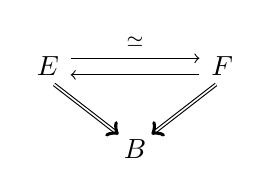
\begin{tikzpicture}[x=1.5em,y=1.5em,baseline=(current bounding box.center)]
  \node (E) at (0,0.9) {$E$};
  \node (F) at (4.2,0.9) {$F$};
  \node (B) at (2.1,-1.1) {$B$};
  \draw[->] (0.55,1.08) -- (3.65,1.08);
  \node at (2.1,1.48) {$\scriptstyle\simeq$};
  \draw[->] (3.65,0.68) -- (0.55,0.68);
  \draw[double,->] (0.15,0.45) -- (1.7,-0.75);
  \draw[double,->] (4.05,0.45) -- (2.5,-0.75);
\end{tikzpicture}
\end{rveq}
我们记 $E\simeq_{B}F$，以指明带这些定义域的指定诸等价纤维化\emph{在} $B$ \emph{上}%
等价。
\end{definition}

由命题 1.2.22(vii)，\trFiberedEquivalence{}无非是公共底上的一对等价纤维化之间的、在底%
\trInfinityCosmos{}中构成\trEquivalence{}的一个映射：遗忘函子 $\mathcal{K}_{/B}\to\mathcal{K}$%
保持且反射诸\trEquivalence{}。
然而请注意，它并不创造它们：两个\trInfinityCategory{} $E$ 与 $F$ 完全可能相互等价，%
却不存在任何与指定等价纤维化对 $E\twoheadrightarrow B$、$F\twoheadrightarrow B$%
相容的\trEquivalence{}。

\begin{warning}\label{war:fibered-equivalence-presentation}
至此，关于在\trInfinityCosmos{} $\mathcal{K}_{/B}$ 中呈现一条\trFiberedEquivalence{}所需的 2-范畴论%
数据为何，尚存某种含混；这与练习 1.4.vii 就 2-范畴 $\mathrm{h}(\mathcal{K}_{/B})$ 与%
$(\mathrm{h}\mathcal{K})_{/B}$ 之间的关系所提出的问题是相关的。
但由于命题 1.2.22(vii) 告诉我们，$\mathrm{h}\mathcal{K}$ 中单单一个涉及形如%
\eqref{eq:fibered-equivalence} 之\trFunctor{}的\trEquivalence{}便已足以保证这项目前%
尚未指明的 2-范畴论数据存在，故我们把这个问题的细致分析推迟到命题 3.6.4。
\end{warning}

\begin{proposition}[\trArrowInfinityCategory{}的唯一性]\label{prop:arrow-category-uniqueness}
对任何\trFiberedEquivalence{}于 $(p_{1},p_{0})\colon A^{2}\twoheadrightarrow A\times A$ 的%
等价纤维化 $(e_{1},e_{0})\colon E\twoheadrightarrow A\times A$，由\trEquivalence{}%
$e\colon E\rightleftarrows A^{2}$ 所编码的 2-\trCell
\begin{center}
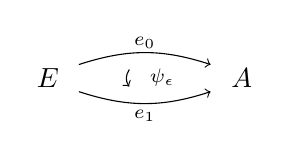
\begin{tikzpicture}[x=1.4em,y=1.4em]
  \node (a) at (0,0) {$E$};
  \node (b) at (5,0) {$A$};
  \draw[->] (0.8,0.35) to[bend left=18] (4.2,0.35);
  \node at (2.5,0.92) {$\scriptstyle e_{0}$};
  \draw[->] (0.8,-0.35) to[bend right=18] (4.2,-0.35);
  \node at (2.5,-0.97) {$\scriptstyle e_{1}$};
  \draw[->] (2.1,0.22) to[bend right=35] (2.1,-0.22);
  \node at (2.95,0.0) {$\scriptstyle\psi_{\epsilon}$};
\end{tikzpicture}
\end{center}
满足\cref{prop:weak-universal-property}的弱\trUniversalProperty{}。反之，若等价纤维化%
$(d_{1},d_{0})\colon D\twoheadrightarrow A\times A$ 与 $(e_{1},e_{0})\colon E\twoheadrightarrow A\times A$%
配备有 2-\trCell
\begin{center}
\begin{tikzpicture}[x=1.4em,y=1.4em]
  \node (a) at (0,0) {$D$};
  \node (b) at (5,0) {$A$};
  \draw[->] (0.8,0.35) to[bend left=18] (4.2,0.35);
  \node at (2.5,0.92) {$\scriptstyle d_{0}$};
  \draw[->] (0.8,-0.35) to[bend right=18] (4.2,-0.35);
  \node at (2.5,-0.97) {$\scriptstyle d_{1}$};
  \draw[->] (2.1,0.22) to[bend right=35] (2.1,-0.22);
  \node at (2.95,0.0) {$\scriptstyle\psi_{\delta}$};
  \node at (8.6,0) {与};
  \begin{scope}[shift={(12.2,0)}]
  \node (a) at (0,0) {$E$};
  \node (b) at (5,0) {$A$};
  \draw[->] (0.8,0.35) to[bend left=18] (4.2,0.35);
  \node at (2.5,0.92) {$\scriptstyle e_{0}$};
  \draw[->] (0.8,-0.35) to[bend right=18] (4.2,-0.35);
  \node at (2.5,-0.97) {$\scriptstyle e_{1}$};
  \draw[->] (2.1,0.22) to[bend right=35] (2.1,-0.22);
  \node at (2.95,0.0) {$\scriptstyle\psi_{\epsilon}$};
  \end{scope}
\end{tikzpicture}
\end{center}
且它们满足\cref{prop:weak-universal-property}的弱\trUniversalProperty{}，则%
$D\simeq_{A\times A}E$。
\end{proposition}

\begin{proof}
我们证明第一个陈述。由 1-\trCell{}归纳的定义等式 $\epsilon=\kappa e$，其中 $\kappa$ 是%
\trGenericArrow \eqref{eq:generic-arrow}。于是，与 $\epsilon$ 作粘贴所诱导的\trFunctor{}分解为%
一个复合
\begin{center}
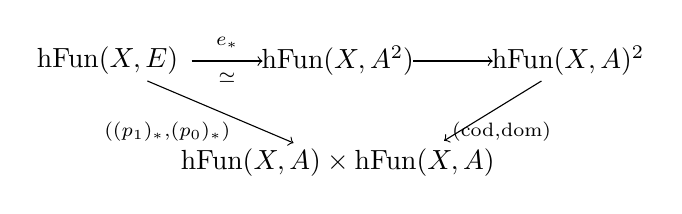
\begin{tikzpicture}[x=1.6em,y=1.6em]
  \node (l) at (0,1.3) {$\mathrm{hFun}(X,E)$};
  \node (m) at (5.2,1.3) {$\mathrm{hFun}(X,A^{2})$};
  \node (r) at (10.4,1.3) {$\mathrm{hFun}(X,A)^{2}$};
  \node (bm) at (5.2,-1.0) {$\mathrm{hFun}(X,A)\times\mathrm{hFun}(X,A)$};
  \draw[->] (1.9,1.3) -- (3.5,1.3);
  \node at (2.7,1.72) {$\scriptstyle e_{*}$};
  \node at (2.7,0.92) {$\scriptstyle\simeq$};
  \draw[->] (6.9,1.3) -- (8.7,1.3);
  \draw[->] (0.9,0.85) -- (4.2,-0.55);
  \node at (1.35,-0.3) {$\scriptstyle((p_{1})_{*},(p_{0})_{*})$};
  \draw[->] (9.8,0.85) -- (7.6,-0.5);
  \node at (8.9,-0.3) {$\scriptstyle(\mathrm{cod},\mathrm{dom})$};
\end{tikzpicture}
\end{center}
而我们的任务是证明该复合\trFunctor{}是\trSmothering{}。第一个\trFunctor{}由与%
\trEquivalence{} $e\colon E\rightleftarrows A^{2}$ 作后复合定义，是\trCategory{}之间的%
一个\trEquivalence{}；第二个\trFunctor{}则是\trSmothering{}。于是，该复合显然\trFull{}且%
\trConservative{}。为见它也对象上满，先注意由 1-\trCell{}归纳，任何 2-\trCell
\begin{center}
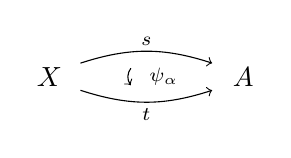
\begin{tikzpicture}[x=1.4em,y=1.4em]
  \node (a) at (0,0) {$X$};
  \node (b) at (5,0) {$A$};
  \draw[->] (0.8,0.35) to[bend left=18] (4.2,0.35);
  \node at (2.5,0.92) {$\scriptstyle s$};
  \draw[->] (0.8,-0.35) to[bend right=18] (4.2,-0.35);
  \node at (2.5,-0.97) {$\scriptstyle t$};
  \draw[->] (2.1,0.22) to[bend right=35] (2.1,-0.22);
  \node at (2.95,0.0) {$\scriptstyle\psi_{\alpha}$};
\end{tikzpicture}
\end{center}
都由 $A\times A$ 之上的某个\trFunctor{} $\qcor{\alpha^{+}}\colon X\to A^{2}$ 所表示。%
与 $e$ 的任一\trFiberedInverseEquivalence $e'$ 作复合，便给出\trFunctor
\begin{center}
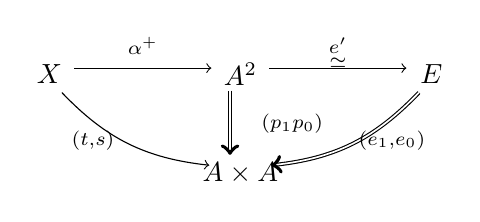
\begin{tikzpicture}[x=1.5em,y=1.5em]
  \node (X) at (0,0) {$X$};
  \node (M) at (4.6,0) {$A^{2}$};
  \node (E) at (9.2,0) {$E$};
  \node (B) at (4.6,-2.4) {$A\times A$};
  \draw[->] (0.6,0.14) -- (3.9,0.14);
  \node at (2.25,0.68) {$\scriptstyle\ulcorner\alpha^{+}\urcorner$};
  \draw[->] (5.3,0.14) -- (8.6,0.14);
  \node at (6.95,0.68) {$\scriptstyle e'$};
  \node at (6.95,0.26) {$\scriptstyle\simeq$};
  \draw[double,->] (4.35,-0.4) -- (4.35,-1.95);
  \node at (5.85,-1.2) {$\scriptstyle(p_{1}p_{0})$};
  \draw[->] (0.3,-0.45) to[bend right=20] (3.85,-2.2);
  \node at (1.05,-1.6) {$\scriptstyle(t,s)$};
  \draw[double,->] (8.9,-0.45) to[bend left=20] (5.35,-2.2);
  \node at (8.25,-1.6) {$\scriptstyle(e_{1},e_{0})$};
\end{tikzpicture}
\end{center}
其在与 $e$ 作\trPostComposition{}之后的像，与 $A\times A$ 之上的 $\qcor{\alpha^{+}}$%
\trFiberedIsomorphism{}。由于这一同构在\cref{prop:whiskering-bijection}的意义下是\trFibered{}，%
$e'\qcor{\alpha^{+}}$ 在\trFunctor{} $\mathrm{hFun}(X,E)\to\mathrm{hFun}(X,A)^{2}$ 之下的%
像便还原出 2-\trCell{} $\alpha$。这便证明了该映射对象上满，从而如所宣称的那样定义了%
一个\trSmotheringFunctor{}。反方向则留作\cref{ex:converse-of-uniqueness}，并将在更一般的%
语境中于命题 3.4.11 得证。
\end{proof}

\begin{convention}\label{conv:arrow-infinity-category-appellation}
由于\cref{prop:arrow-category-uniqueness}，我们把「\trArrowInfinityCategory」这一称谓从%
\cref{def:arrow-infinity-category}所构造的严格模型扩充到任何\trFiberedEquivalence{}于它的%
\trInfinityCategory{}。
\end{convention}

经\cref{lem:smothering-free}，本节的结果可扩充为：\trInfinityCategory{} $A$ 与\trFreeCategory{} $J$ 之%
余张量 $A^{J}$ 的相应弱\trUniversalProperty——邀请读者自行探索。

\subsection*{练习}

\begin{exercise}\label{ex:arrow-representations}
本练习重温\cref{prop:whiskering-bijection}的结果。
\begin{enumerate}[label=(\roman*)]
\item 证明：\trQuasiCategory{} $Q$ 中一对平行的 1-\trSimplex{} $f,g\colon x\to y$ 是%
\trHomotopic{}，当且仅当作为 $Q^{2}$ 的\trElement{}，二者经由一个沿 $(p_{1},p_{0})\colon Q^{2}\twoheadrightarrow Q\times Q$%
投影为恒同的\trIsomorphism{}而\trIsomorphism{}。
\item 由此推出：任一\trInfinityCosmos{}中两个\trInfinityCategory{} $X$ 与 $A$ 之间%
\trFunctorSpace{}里的一对平行 1-箭头表示同一\trNaturalTransformation{}，当且仅当作为%
$\mathrm{Fun}(X,A)^{2}\cong\mathrm{Fun}(X,A^{2})$ 的\trElement{}，二者经由一个定义域%
分量与余定义域分量皆为恒同的\trIsomorphism{}而\trIsomorphism{}。
\item 再由此推出：$\mathrm{Fun}(X,A)$ 中一对平行的 1-箭头——它们可编码为\trFunctor{}%
$X\to A^{2}$——表示同一\trNaturalTransformation{}，当且仅当二者由一个\trFiberedIsomorphism{}相连：%
\begin{center}
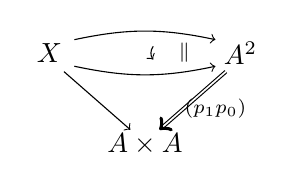
\begin{tikzpicture}[x=1.5em,y=1.5em]
  \node (X) at (0,0) {$X$};
  \node (M) at (4.6,0) {$A^{2}$};
  \node (B) at (2.3,-2.2) {$A\times A$};
  \draw[->] (0.6,0.32) to[bend left=12] (4.0,0.32);
  \draw[->] (0.6,-0.32) to[bend right=12] (4.0,-0.32);
  \draw[->] (2.5,0.16) to[bend right=35] (2.5,-0.16);
  \node at (3.25,0.0) {$\scriptstyle\parallel$};
  \draw[->] (0.35,-0.45) -- (1.95,-1.85);
  \draw[double,->] (4.25,-0.45) -- (2.65,-1.85);
  \node at (4.0,-1.35) {$\scriptstyle(p_{1}p_{0})$};
\end{tikzpicture}
\end{center}
\end{enumerate}
\end{exercise}

\begin{exercise}\label{ex:converse-of-uniqueness}
证明\cref{prop:arrow-category-uniqueness}的逆蕴含。
\end{exercise}

\begin{exercise}\label{ex:cotensor-weak-universal-property}
把\cref{prop:weak-universal-property}与\cref{prop:whiskering-bijection}的结果
推广到：由某个\trReflexiveDirectedGraph{}自由生成的\trCategory{} $J$ 的%
\trInfinityCategory{} $A$ 的余张量 $A^J$ 的弱泛性质。
\end{exercise}

   %

\section{\trIsofibration{}的\trPullback}\label{sec:pullbacks-of-isofibrations}

\trInfinityCosmos{}中\trIsofibration{}之塔的\trPullback{}与\trLimit{}在%
\trHomotopyTwoCategory{}中也具有弱 2 维\trUniversalProperty，不过我们通常转而%
利用\trSimpliciallyEnrichedLimit{}的严格\trUniversalProperty。然而，%
\trPullback{}的弱 2 维\trUniversalProperty{}可用于证明：\trEquivalence{}沿%
\trIsofibration{}拉回后仍是\trEquivalence{}；而这又可用于确立%
\trInfinityCosmos{}中\trPullback{}的\trEquivalence{}不变性。

\begin{proposition}[\trPullback{}的弱\trUniversalProperty]\label{prop:pullback-weak-universal-property}
\trInfinityCosmos{}中沿一个\trFunctor{}的\trIsofibration{}之\trPullback%
\begin{center}
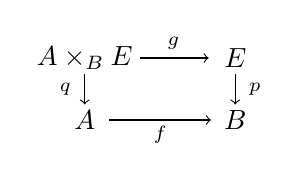
\begin{tikzpicture}[x=1.6em,y=1.6em]
  \node (tl) at (0,1.4) {$A\times_BE$};
  \node (tr) at (3.4,1.4) {$E$};
  \node (bl) at (0,0) {$A$};
  \node (br) at (3.4,0) {$B$};
  \draw[->] (1.25,1.4) -- (2.8,1.4);
  \node at (2.0,1.74) {$\scriptstyle g$};
  \draw[->] (0,1.05) -- (0,0.35);
  \node at (-0.44,0.7) {$\scriptstyle q$};
  \node at (0.48,0.78) {$\scriptstyle\lrcorner$};
  \draw[->] (3.4,1.05) -- (3.4,0.35);
  \node at (3.84,0.7) {$\scriptstyle p$};
  \draw[->] (0.55,0) -- (2.85,0);
  \node at (1.7,-0.34) {$\scriptstyle f$};
\end{tikzpicture}
\end{center}
在\trHomotopyTwoCategory{}中具有由下述三种运算给出的弱\trUniversalProperty{}：
\begin{enumerate}[label=(\roman*)]
\item \textbf{1-\trCell{}归纳：}在拉回图表所赖的\trCospan{}上方，满足%
$pe=f\alpha$ 的交换方块都唯一地穿过拉回方块分解
\begin{center}
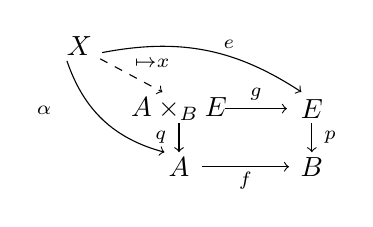
\begin{tikzpicture}[x=1.5em,y=1.5em]
  \node (X) at (0,2.9) {$X$};
  \node (tl) at (2.4,1.4) {$A\times_BE$};
  \node (tr) at (5.6,1.4) {$E$};
  \node (bl) at (2.4,0) {$A$};
  \node (br) at (5.6,0) {$B$};
  \draw[->,dashed] (0.5,2.6) -- (2.0,1.8);
  \node at (1.75,2.5) {$\scriptstyle\mapsto x$};
  \draw[->] (0.55,2.75) to[bend left=22] (5.35,1.8);
  \node at (3.6,2.95) {$\scriptstyle e$};
  \draw[->] (-0.3,2.55) to[bend right=28] (2.05,0.35);
  \node at (-0.85,1.35) {$\scriptstyle\alpha$};
  \draw[->] (3.5,1.4) -- (5.0,1.4);
  \node at (4.25,1.74) {$\scriptstyle g$};
  \draw[->] (2.4,1.05) -- (2.4,0.35);
  \node at (1.96,0.7) {$\scriptstyle q$};
  \node at (2.88,0.78) {$\scriptstyle\lrcorner$};
  \draw[->] (5.6,1.05) -- (5.6,0.35);
  \node at (6.04,0.7) {$\scriptstyle p$};
  \draw[->] (2.95,0) -- (5.05,0);
  \node at (4.0,-0.34) {$\scriptstyle f$};
\end{tikzpicture}
\end{center}
\item \textbf{2-\trCell{}归纳：}给定\trFunctor{} $x,x'\colon X\to A\times_BE$ 与%
\trNaturalTransformation{} $\alpha\colon qx\Rightarrow qx'$、%
$\epsilon\colon gx\Rightarrow gx'$，使得 $p\epsilon=f\alpha$，则存在%
\trNaturalTransformation{} $\tau\colon x\Rightarrow x'$，使得 $q\tau=\alpha$%
且 $g\tau=\epsilon$。
\item \textbf{2-\trCell{}保守性：}对任何
\begin{center}
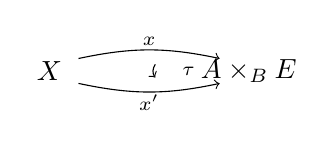
\begin{tikzpicture}[x=1.5em,y=1.5em]
  \node (X) at (0,0) {$X$};
  \node (M) at (4.8,0) {$A\times_BE$};
  \draw[->] (0.7,0.3) to[bend left=12] (4.1,0.3);
  \node at (2.4,0.72) {$\scriptstyle x$};
  \draw[->] (0.7,-0.3) to[bend right=12] (4.1,-0.3);
  \node at (2.4,-0.76) {$\scriptstyle x'$};
  \draw[->] (2.55,0.16) to[bend right=35] (2.55,-0.16);
  \node at (3.35,0.0) {$\scriptstyle\tau$};
\end{tikzpicture}
\end{center}
若 $q\tau$ 与 $g\tau$ 皆为\trIsomorphism{}，则 $\tau$ 是\trIsomorphism{}。
\end{enumerate}
\end{proposition}

\begin{proof}
对由\trQuasiCategory{}构成的如下\trPullback{}图表应用引理 3.1.5
\begin{center}
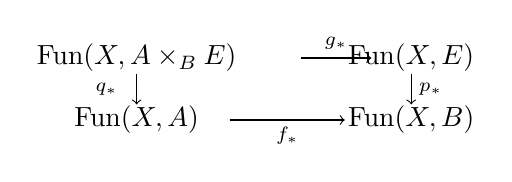
\begin{tikzpicture}[x=1.6em,y=1.6em]
  \node (tl) at (0,1.4) {$\mathrm{Fun}(X,A\times_BE)$};
  \node (tr) at (6.2,1.4) {$\mathrm{Fun}(X,E)$};
  \node (bl) at (0,0) {$\mathrm{Fun}(X,A)$};
  \node (br) at (6.2,0) {$\mathrm{Fun}(X,B)$};
  \draw[->] (3.7,1.4) -- (5.3,1.4);
  \node at (4.5,1.74) {$\scriptstyle g_{*}$};
  \draw[->] (0,1.05) -- (0,0.35);
  \node at (-0.68,0.7) {$\scriptstyle q_{*}$};
  \node at (0.48,0.78) {$\scriptstyle\lrcorner$};
  \draw[->] (6.2,1.05) -- (6.2,0.35);
  \node at (6.64,0.7) {$\scriptstyle p_{*}$};
  \draw[->] (2.1,0) -- (4.7,0);
  \node at (3.4,-0.36) {$\scriptstyle f_{*}$};
\end{tikzpicture}
\end{center}
即可观察到：\trHomCategory{}之间的自然映射
\[
\mathrm{hFun}(X,A\times_BE)\longrightarrow
\mathrm{hFun}(X,A)\times_{\mathrm{hFun}(X,B)}\mathrm{hFun}(X,E)
\]
是一个对象上双射的\trSmotheringFunctor{}。对象上的双射性由 1-\trCell{}归纳%
表达，满性由 2-\trCell{}归纳表达，而保守性由 2-\trCell{}保守性表达。
\end{proof}

\begin{digression}[\trWeaklyCartesianSquare]\label{dig:weakly-cartesian-squares}
平行\trIsofibration{}之间的一个交换方块是\textbf{\trWeaklyCartesian}%
（weakly cartesian），若其到\trPullback{}的诱导映射是一个\trEquivalence{}：
\begin{center}
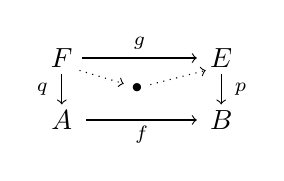
\begin{tikzpicture}[x=1.6em,y=1.6em]
  \node (tl) at (0,1.4) {$F$};
  \node (tr) at (3.6,1.4) {$E$};
  \node (bl) at (0,0) {$A$};
  \node (br) at (3.6,0) {$B$};
  \draw[->] (0.45,1.4) -- (3.05,1.4);
  \node at (1.75,1.74) {$\scriptstyle g$};
  \draw[->] (0,1.05) -- (0,0.35);
  \node at (-0.44,0.7) {$\scriptstyle q$};
  \draw[->] (3.6,1.05) -- (3.6,0.35);
  \node at (4.04,0.7) {$\scriptstyle p$};
  \draw[->] (0.55,0) -- (3.05,0);
  \node at (1.8,-0.34) {$\scriptstyle f$};
  \draw[->,dotted] (0.4,1.12) -- (1.4,0.82);
  \draw[->,dotted] (2.0,0.8) -- (3.25,1.12);
  \node at (1.7,0.72) {$\scriptstyle\bullet$};
  \node at (2.25,0.5) {$\scriptstyle\lrcorner$};
\end{tikzpicture}
\end{center}
\trWeaklyCartesianSquare{}同样满足 2-\trCell{}归纳与 2-\trCell{}保守性，还%
满足一种经过修改的 1-\trCell{}归纳性质：此时本质唯一的诱导\trFunctor{}在%
$B$ 上严格交换，而在 $E$ 上至多相差一个同构——该同构沿 $p$ 投影为恒同——%
[110, 3.5.4]。
\end{digression}

由\trPullback{}的\trBicategory\trUniversalProperty{}可以推出：\trInfinityCosmos{}%
都是\textbf{\trRightProper}（right proper）——意即任何\trEquivalence{}沿%
\trIsofibration{}的\trPullback{}都定义出一个\trEquivalence{}。

\begin{proposition}\label{prop:pullback-equivalence}
在任何\trInfinityCosmos{}中，\trEquivalence{}沿\trIsofibration{}的%
\trPullback{}是一个\trEquivalence{}。
\begin{center}
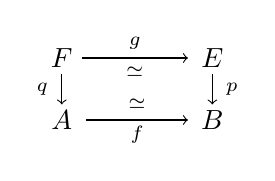
\begin{tikzpicture}[x=1.6em,y=1.6em]
  \node (tl) at (0,1.4) {$F$};
  \node (tr) at (3.4,1.4) {$E$};
  \node (bl) at (0,0) {$A$};
  \node (br) at (3.4,0) {$B$};
  \draw[->] (0.45,1.4) -- (2.85,1.4);
  \node at (1.65,1.74) {$\scriptstyle g$};
  \node at (1.65,1.08) {$\scriptstyle\simeq$};
  \draw[->] (0,1.05) -- (0,0.35);
  \node at (-0.44,0.7) {$\scriptstyle q$};
  \node at (0.48,0.78) {$\scriptstyle\lrcorner$};
  \draw[->] (3.4,1.05) -- (3.4,0.35);
  \node at (3.84,0.7) {$\scriptstyle p$};
  \draw[->] (0.55,0) -- (2.85,0);
  \node at (1.7,-0.34) {$\scriptstyle f$};
  \node at (1.7,0.36) {$\scriptstyle\simeq$};
\end{tikzpicture}
\end{center}
\end{proposition}

\begin{proof}
由命题 2.1.12，我们可以选取 $f$ 的一个\trAdjointEquivalence{}逆 $f^{-1}$，并%
挑选可逆 2-\trCell{} $\alpha\colon\mathrm{id}_A\cong f^{-1}f$ 与%
$\beta\colon ff^{-1}\cong\mathrm{id}_B$，使之在\trHomotopyTwoCategory{}中%
满足\trTriangleEqualities{}。\footnote{正是因为这一点，我们使用的才是拉回的%
\trBicategory\trUniversalProperty，而非单纯富集的\trUniversalProperty。}
既然映射 $p$ 是\trIsofibration{}，我们便可利用命题 1.4.9 把同构%
$\beta p\colon ff^{-1}p\cong p$ 沿 $p$ 提升，以定义一个\trIsomorphism{}%
$\epsilon\colon e\cong\mathrm{id}_E$，其余定义域为 $\mathrm{id}_E\colon E\to E$。%
由构造有 $pe=ff^{-1}p$，故由 1-\trCell{}归纳，对 $(f^{-1}p,e)$ 便诱导出映射%
$g^{-1}\colon E\to F$，使得 $qg^{-1}=f^{-1}p$ 且 $gg^{-1}=e$。这样我们便%
得到一个\trIsomorphism{} $\epsilon\colon gg^{-1}\cong\mathrm{id}_E$，满足%
$p\epsilon=\beta p$。

现在，据\cref{prop:pullback-weak-universal-property}的 2-\trCell{}归纳与%
保守性，为定义一个\trIsomorphism{} $\mathrm{id}_F\cong g^{-1}g$，只需给出%
如下一对\trIsomorphism
\[
\alpha q\colon q\cong f^{-1}fq=f^{-1}pg=qg^{-1}g
\qquad\text{以及}\qquad
\epsilon^{-1}g\colon g\cong gg^{-1}g
\]
使得 $f\alpha q=p\epsilon^{-1}g$。后一等式之所以成立，是因为对%
\trAdjointEquivalence{} $f\dashv f^{-1}$ 而言，据三角等式%
$\beta f\cdot f\alpha=\mathrm{id}_f$，有%
$p\epsilon^{-1}g=\beta^{-1}pg=\beta^{-1}fq=f\alpha q$。于是，我们可以把 $f$ %
的逆\trEquivalence{}数据加以提升，以定义其\trPullback{} $g$ 的%
逆\trEquivalence{}。
\end{proof}

作为\trRightProperness{}的推论，在任何\trInfinityCosmos{}中，\trPullback{}%
都是一个\trEquivalence{}不变的构造。

\begin{proposition}\label{prop:pullback-invariance}
给定任意\trInfinityCosmos{}中一个由\trIsofibration{}与\trEquivalence{}构成%
的\trDiagram
\begin{center}
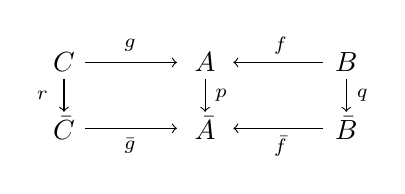
\begin{tikzpicture}[x=1.7em,y=1.7em]
  \node (tl) at (0,1.4) {$C$};
  \node (tm) at (3.0,1.4) {$A$};
  \node (tr) at (6.0,1.4) {$B$};
  \node (bl) at (0,0) {$\bar{C}$};
  \node (bm) at (3.0,0) {$\bar{A}$};
  \node (brr) at (6.0,0) {$\bar{B}$};
  \draw[->] (0.45,1.4) -- (2.4,1.4);
  \node at (1.4,1.76) {$\scriptstyle g$};
  \draw[->] (5.5,1.4) -- (3.6,1.4);
  \node at (4.6,1.76) {$\scriptstyle f$};
  \draw[->] (0.45,0) -- (2.4,0);
  \node at (1.4,-0.38) {$\scriptstyle\bar{g}$};
  \draw[->] (5.5,0) -- (3.6,0);
  \node at (4.6,-0.38) {$\scriptstyle\bar{f}$};
  \draw[->] (0,1.05) -- (0,0.35);
  \node at (-0.46,0.7) {$\scriptstyle r$};
  \draw[->] (3.0,1.05) -- (3.0,0.35);
  \node at (3.34,0.7) {$\scriptstyle p$};
  \draw[->] (6.0,1.05) -- (6.0,0.35);
  \node at (6.34,0.7) {$\scriptstyle q$};
\end{tikzpicture}
\end{center}
上下两行各自的\trPullback{}之间的诱导映射%
$C\times_AB\to\bar{C}\times_{\bar{A}}\bar{B}$ 仍是\trEquivalence{}。
\end{proposition}

\begin{proof}
利用引理 1.2.19 作因子分解，我们可以把映射 $\bar{g}$ 替换成一个%
\trIsofibration{}。据\trTwoOfThreeProperty{}与%
\cref{prop:pullback-equivalence}的\trRightProperness，该\trIsofibration{}沿%
\trEquivalence{} $p$ 的\trPullback{}便\trEquivalence{}于映射 $g$：
\begin{center}
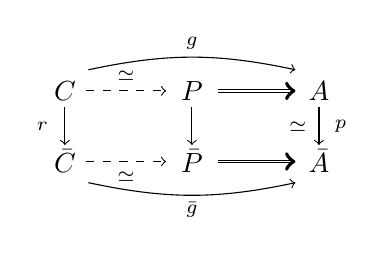
\begin{tikzpicture}[x=1.7em,y=1.7em]
  \node (C) at (0,1.4) {$C$};
  \node (P) at (2.7,1.4) {$P$};
  \node (A) at (5.4,1.4) {$A$};
  \node (Cb) at (0,-0.1) {$\bar{C}$};
  \node (Pb) at (2.7,-0.1) {$\bar{P}$};
  \node (Ab) at (5.4,-0.1) {$\bar{A}$};
  \draw[->] (0.5,1.85) to[bend left=12] (4.9,1.85);
  \node at (2.7,2.42) {$\scriptstyle g$};
  \draw[->] (0.5,-0.55) to[bend right=12] (4.9,-0.55);
  \node at (2.7,-1.12) {$\scriptstyle\bar{g}$};
  \draw[->,dashed] (0.45,1.4) -- (2.15,1.4);
  \node at (1.3,1.72) {$\scriptstyle\simeq$};
  \draw[double,->] (3.25,1.4) -- (4.9,1.4);
  \draw[->,dashed] (0.45,-0.1) -- (2.15,-0.1);
  \node at (1.3,-0.42) {$\scriptstyle\simeq$};
  \draw[double,->] (3.25,-0.1) -- (4.9,-0.1);
  \draw[->] (0,1.05) -- (0,0.25);
  \node at (-0.48,0.65) {$\scriptstyle r$};
  \draw[->] (2.7,1.05) -- (2.7,0.25);
  \draw[->] (5.4,1.05) -- (5.4,0.25);
  \node at (5.86,0.65) {$\scriptstyle p$};
  \node at (4.95,0.65) {$\scriptstyle\simeq$};
  \node at (3.2,1.02) {$\scriptstyle\lrcorner$};
\end{tikzpicture}
\end{center}
\begin{center}
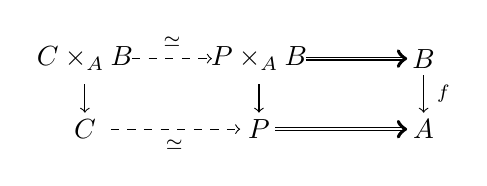
\begin{tikzpicture}[x=1.7em,y=1.7em]
  \node (Cg) at (0,1.4) {$C\times_AB$};
  \node (Pg) at (3.7,1.4) {$P\times_AB$};
  \node (B)  at (7.2,1.4) {$B$};
  \node (C)  at (0,-0.1) {$C$};
  \node (P)  at (3.7,-0.1) {$P$};
  \node (A)  at (7.2,-0.1) {$A$};
  \draw[->,dashed] (1.0,1.4) -- (2.7,1.4);
  \node at (1.85,1.76) {$\scriptstyle\simeq$};
  \draw[double,->] (4.7,1.4) -- (6.85,1.4);
  \draw[->,dashed] (0.55,-0.1) -- (3.3,-0.1);
  \node at (1.9,-0.42) {$\scriptstyle\simeq$};
  \draw[double,->] (4.05,-0.1) -- (6.85,-0.1);
  \draw[->] (0,0.85) -- (0,0.25);
  \draw[->] (3.7,0.85) -- (3.7,0.25);
  \draw[->] (7.2,1.05) -- (7.2,0.25);
  \node at (7.62,0.65) {$\scriptstyle f$};
  \node at (0.9,0.8) {$\scriptstyle\lrcorner$};
  \node at (4.6,0.8) {$\scriptstyle\lrcorner$};
\end{tikzpicture}
\end{center}

再由\trRightProperness，$P\twoheadrightarrow A$ 沿 $f$ 的\trPullback{}与%
$g\colon C\to A$ 沿 $f$ 的\trPullback{}\trEquivalence{}，对下方水平映射%
亦然。于是不失一般性，我们可以假设题设中的映射 $g$ 与 $\bar{g}$ 都是%
\trIsofibration{}，而且左手方块是一个\trPullback{}。

在这些新假设之下，立方体的顶面、底面与正面都是拉回方块：
\begin{center}
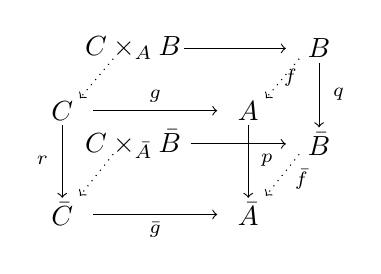
\begin{tikzpicture}[x=1.6em,y=1.5em]
  \node (Btl) at (1.6,4.0) {$C\times_AB$};
  \node (Btr) at (5.8,4.0) {$B$};
  \node (Bbl) at (1.6,1.7) {$C\times_{\bar{A}}\bar{B}$};
  \node (Bbr) at (5.8,1.7) {$\bar{B}$};
  \node (Ftl) at (0,2.5) {$C$};
  \node (Ftr) at (4.2,2.5) {$A$};
  \node (Fbl) at (0,0) {$\bar{C}$};
  \node (Fbr) at (4.2,0) {$\bar{A}$};
  \draw[->] (0.7,2.5) -- (3.5,2.5);
  \node at (2.1,2.85) {$\scriptstyle g$};
  \draw[->] (0.7,0) -- (3.5,0);
  \node at (2.1,-0.36) {$\scriptstyle\bar{g}$};
  \draw[->] (0,2.15) -- (0,0.4);
  \node at (-0.45,1.3) {$\scriptstyle r$};
  \draw[->] (4.2,2.15) -- (4.2,0.4);
  \node at (4.62,1.3) {$\scriptstyle p$};
  \draw[->] (2.75,4.0) -- (5.05,4.0);
  \draw[->] (2.9,1.7) -- (5.05,1.7);
  \draw[->] (5.8,3.65) -- (5.8,2.1);
  \node at (6.24,2.9) {$\scriptstyle q$};
  \draw[->,dotted] (1.15,3.75) -- (0.4,2.8);
  \draw[->,dotted] (5.35,3.75) -- (4.6,2.8);
  \node at (5.15,3.3) {$\scriptstyle f$};
  \draw[->,dotted] (1.15,1.45) -- (0.4,0.45);
  \draw[->,dotted] (5.35,1.45) -- (4.6,0.45);
  \node at (5.4,0.85) {$\scriptstyle\bar{f}$};
  \node at (2.2,3.62) {$\scriptstyle\lrcorner$};
  \node at (0.48,2.12) {$\scriptstyle\lrcorner$};
  \node at (2.2,1.32) {$\scriptstyle\lrcorner$};
\end{tikzpicture}
\end{center}
故由拉回的复合与消去，背面也是一个拉回方块。此时，诱导映射%
$C\times_AB\to\bar{C}\times_{\bar{A}}\bar{B}$ 是等价 $q$ 沿一个%
\trIsofibration{}的\trPullback{}，从而据\cref{prop:pullback-equivalence}是%
\trEquivalence{}。
\end{proof}

\subsection*{练习}

\begin{exercise}\label{ex:pullback-isomorphic-functors}
利用\cref{prop:pullback-weak-universal-property}证明：对任何%
\trIsofibration{}以及一对平行的、相互\trIsomorphism{}的\trFunctor
\begin{center}
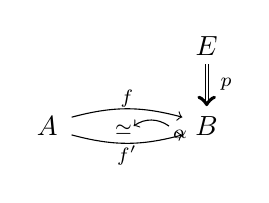
\begin{tikzpicture}[x=1.6em,y=1.6em]
  \node (A) at (0,0) {$A$};
  \node (B) at (3.6,0) {$B$};
  \node (E) at (3.6,1.8) {$E$};
  \draw[double,->] (3.6,1.4) -- (3.6,0.45);
  \node at (4.04,0.95) {$\scriptstyle p$};
  \draw[->] (0.55,0.2) to[bend left=15] (3.05,0.2);
  \node at (1.8,0.62) {$\scriptstyle f$};
  \draw[->] (0.55,-0.2) to[bend right=15] (3.05,-0.2);
  \node at (1.8,-0.66) {$\scriptstyle f'$};
  \draw[->] (2.75,0.0) to[bend right=35] (1.95,0.0);
  \node at (3.0,-0.18) {$\scriptstyle\alpha$};
  \node at (1.72,-0.08) {$\scriptstyle\simeq$};
\end{tikzpicture}
\end{center}
它们的\trPullback{}在 $A$ 上\trEquivalence{}。
\end{exercise}

\begin{exercise}\label{ex:towers-weak-universal-property}
陈述并证明一个与\cref{prop:pullback-weak-universal-property}相类似的结果，刻画%
\trIsofibration{}之塔的\trLimit{}的\trBicategory\trUniversalProperty。
\end{exercise}

\begin{exercise}\label{ex:towers-limits-equivalence}
利用\cref{ex:towers-weak-universal-property}的结果证明：\trIsofibration{}之塔之间的%
一个自然\trEquivalence{}——通过改编\cref{prop:pullback-equivalence}与%
\cref{prop:pullback-invariance}的证明中所给出的构造——诱导出它们的\trLimit{}之间的%
一个\trEquivalence。
\end{exercise}
   %
\providecommand{\qcOne}{\mathbf{1}}   %
\providecommand{\qcTwo}{\mathbf{2}}   %
\providecommand{\qcor}[1]{\ulcorner#1\urcorner}   %
\providecommand{\Cat}{\mathcal{C}at}
\providecommand{\QCat}{\mathcal{Q}\mathcal{C}at}

\section{逗号构造}\label{sec:the-comma-construction}

\textbf{\trCommaInfinityCategory}（comma ∞-category）定义为：沿一对余定义域为 $A$ 的%
指定函子，限制\trArrowInfinityCategory{} $A^{2}$ 的定义域与余定义域。

\begin{definition}[\trCommaInfinityCategory]\label{def:comma-infinity-category}
设 $C\xrightarrow{\;g\;}A\xleftarrow{\;f\;}B$ 是由\trInfinityCategory{}构成的%
一个\trDiagram{}。\textbf{\trCommaInfinityCategory}定义为\trSimplicial\trCotensor{} $A^{2}$%
沿 $g\times f$ 的一个\trPullback
\begin{rveq}\label{eq:comma-pullback}
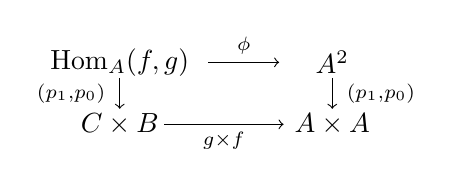
\begin{tikzpicture}[x=1.6em,y=1.6em,baseline=(current bounding box.center)]
  \node (tl) at (0,1.4) {$\mathrm{Hom}_A(f,g)$};
  \node (tr) at (4.8,1.4) {$A^{2}$};
  \node (bl) at (0,0) {$C\times B$};
  \node (br) at (4.8,0) {$A\times A$};
  \draw[->] (2.0,1.4) -- (3.6,1.4);
  \node at (2.8,1.78) {$\scriptstyle\qcor{\phi}$};
  \draw[->] (0,1.05) -- (0,0.35);
  \node at (-1.1,0.7) {$\scriptstyle(p_{1},p_{0})$};
  \node at (0.48,0.78) {$\scriptstyle\lrcorner$};
  \draw[->] (4.8,1.05) -- (4.8,0.35);
  \node at (5.9,0.7) {$\scriptstyle(p_{1},p_{0})$};
  \draw[->] (1.0,0) -- (3.7,0);
  \node at (2.35,-0.36) {$\scriptstyle g\times f$};
\end{tikzpicture}
\end{rveq}
这一构造为\trCommaInfinityCategory{}配备了一个指定的\trIsofibration{}%
$(p_{1},p_{0})\colon\mathrm{Hom}_A(f,g)\twoheadrightarrow C\times B$，以及%
\trHomotopyTwoCategory{}中的一个典范\trNaturalTransformation
\begin{rveq}\label{eq:comma-cone}
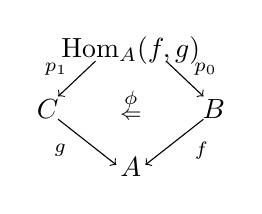
\begin{tikzpicture}[x=1.5em,y=1.5em,baseline=(current bounding box.center)]
  \node (hom) at (0,2.2) {$\mathrm{Hom}_A(f,g)$};
  \node (c) at (-2.0,0.8) {$C$};
  \node (b) at (2.0,0.8) {$B$};
  \node (a) at (0,-0.6) {$A$};
  \draw[->] (-0.85,1.95) -- (-1.75,1.1);
  \node at (-1.8,1.75) {$\scriptstyle p_{1}$};
  \draw[->] (0.85,1.95) -- (1.75,1.1);
  \node at (1.8,1.75) {$\scriptstyle p_{0}$};
  \node at (0,1.02) {$\scriptstyle\phi$};
  \node at (0,0.64) {$\scriptstyle\Leftarrow$};
  \draw[->] (-1.75,0.55) -- (-0.35,-0.55);
  \node at (-1.7,-0.2) {$\scriptstyle g$};
  \draw[->] (1.75,0.55) -- (0.35,-0.55);
  \node at (1.7,-0.2) {$\scriptstyle f$};
\end{tikzpicture}
\end{rveq}
后者称为\textbf{\trCommaCone}（comma cone）。
\end{definition}

由 \eqref{eq:comma-pullback} 的\trUniversalProperty{}，\trCommaInfinityCategory{}的一个\trElement{}%
$(\alpha,b,c)\colon\qcOne\to\mathrm{Hom}_A(f,g)$ 是一个三元组，其中 $b$ 与 $c$ 分别%
是 $B$ 与 $C$ 的\trElement{}，而 $\alpha\colon fb\to gc$ 是 $A$ 中一条以 $fb$ 为定义域、%
以 $gc$ 为余定义域的箭头。

\begin{example}\label{exa:arrows-as-comma}
\trArrowInfinityCategory{}作为应用于恒同\trSpan{}（identity span）的逗号构造的特例而出现。%
这为 \eqref{eq:generic-arrow} 的\trGenericArrow{}提供了另一种记号
\begin{center}
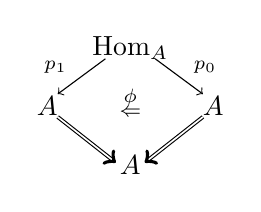
\begin{tikzpicture}[x=1.5em,y=1.5em]
  \node (hom) at (0,2.2) {$\mathrm{Hom}_A$};
  \node (al) at (-2.0,0.8) {$A$};
  \node (ar) at (2.0,0.8) {$A$};
  \node (ab) at (0,-0.6) {$A$};
  \draw[->] (-0.6,1.95) -- (-1.75,1.1);
  \node at (-1.8,1.75) {$\scriptstyle p_{1}$};
  \draw[->] (0.6,1.95) -- (1.75,1.1);
  \node at (1.8,1.75) {$\scriptstyle p_{0}$};
  \node at (0,1.02) {$\scriptstyle\phi$};
  \node at (0,0.64) {$\scriptstyle\Leftarrow$};
  \draw[double,->] (-1.75,0.55) -- (-0.35,-0.55);
  \draw[double,->] (1.75,0.55) -- (0.35,-0.55);
\end{tikzpicture}
\end{center}
它可视为\trCommaCone{}的一个特例。
\end{example}

下列命题编码了逗号构造的诸\trHomotopy{}论性质。

\begin{proposition}[逗号之间的映射]\label{prop:maps-between-commas}
交换\trDiagram
\begin{center}
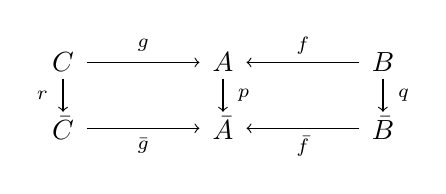
\begin{tikzpicture}[x=1.7em,y=1.7em]
  \node (c) at (0,1.4) {$C$};
  \node (a) at (3.4,1.4) {$A$};
  \node (b) at (6.8,1.4) {$B$};
  \node (cb) at (0,0) {$\bar{C}$};
  \node (ab) at (3.4,0) {$\bar{A}$};
  \node (bb) at (6.8,0) {$\bar{B}$};
  \draw[->] (0.5,1.4) -- (2.9,1.4);
  \node at (1.7,1.76) {$\scriptstyle g$};
  \draw[->] (6.3,1.4) -- (3.9,1.4);
  \node at (5.1,1.76) {$\scriptstyle f$};
  \draw[->] (0.5,0) -- (2.9,0);
  \node at (1.7,-0.38) {$\scriptstyle\bar{g}$};
  \draw[->] (6.3,0) -- (3.9,0);
  \node at (5.1,-0.38) {$\scriptstyle\bar{f}$};
  \draw[->] (0,1.05) -- (0,0.35);
  \node at (-0.44,0.7) {$\scriptstyle r$};
  \draw[->] (3.4,1.05) -- (3.4,0.35);
  \node at (3.84,0.7) {$\scriptstyle p$};
  \draw[->] (6.8,1.05) -- (6.8,0.35);
  \node at (7.24,0.7) {$\scriptstyle q$};
\end{tikzpicture}
\end{center}
诱导出\trCommaInfinityCategory{}之间的一个映射
\begin{center}
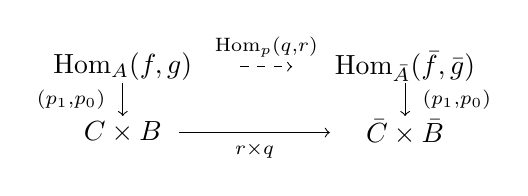
\begin{tikzpicture}[x=1.7em,y=1.7em]
  \node (tl) at (0,1.4) {$\mathrm{Hom}_A(f,g)$};
  \node (tr) at (6.0,1.4) {$\mathrm{Hom}_{\bar{A}}(\bar{f},\bar{g})$};
  \node (bl) at (0,0) {$C\times B$};
  \node (br) at (6.0,0) {$\bar{C}\times\bar{B}$};
  \draw[->,dashed] (2.5,1.4) -- (3.6,1.4);
  \node at (3.05,1.82) {$\scriptstyle\mathrm{Hom}_p(q,r)$};
  \draw[->] (0,1.05) -- (0,0.35);
  \node at (-1.1,0.7) {$\scriptstyle(p_{1},p_{0})$};
  \draw[->] (6.0,1.05) -- (6.0,0.35);
  \node at (7.1,0.7) {$\scriptstyle(p_{1},p_{0})$};
  \draw[->] (1.2,0) -- (4.4,0);
  \node at (2.8,-0.38) {$\scriptstyle r\times q$};
\end{tikzpicture}
\end{center}
此外，若 $p$、$q$ 与 $r$ 全为\trIsofibration{}、全为\trTrivialFibration{}或全为%
\trEquivalence{}，则诱导映射也相应地仍为\trIsofibration{}、\trTrivialFibration{}或%
\trEquivalence{}。
\end{proposition}

\begin{proof}
\trCospan{}之映射给出如下交换\trDiagram
\begin{center}
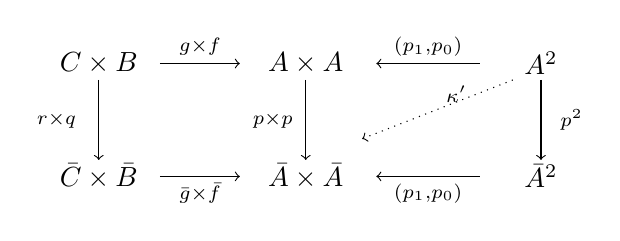
\begin{tikzpicture}[x=1.7em,y=1.7em]
  \node (tl) at (0,1.7) {$C\times B$};
  \node (tm) at (4.4,1.7) {$A\times A$};
  \node (tr) at (9.4,1.7) {$A^{2}$};
  \node (bl) at (0,-0.7) {$\bar{C}\times\bar{B}$};
  \node (bm) at (4.4,-0.7) {$\bar{A}\times\bar{A}$};
  \node (br) at (9.4,-0.7) {$\bar{A}^{2}$};
  \draw[->] (1.3,1.7) -- (3.0,1.7);
  \node at (2.15,2.06) {$\scriptstyle g\times f$};
  \draw[->] (8.1,1.7) -- (5.9,1.7);
  \node at (7.0,2.06) {$\scriptstyle(p_{1},p_{0})$};
  \draw[->] (1.3,-0.7) -- (3.0,-0.7);
  \node at (2.15,-1.06) {$\scriptstyle\bar{g}\times\bar{f}$};
  \draw[->] (8.1,-0.7) -- (5.9,-0.7);
  \node at (7.0,-1.06) {$\scriptstyle(p_{1},p_{0})$};
  \draw[->] (0,1.35) -- (0,-0.35);
  \node at (-0.9,0.5) {$\scriptstyle r\times q$};
  \draw[->] (4.4,1.35) -- (4.4,-0.35);
  \node at (3.7,0.5) {$\scriptstyle p\times p$};
  \draw[->] (9.4,1.35) -- (9.4,-0.35);
  \node at (10.05,0.5) {$\scriptstyle p^{2}$};
  \draw[->,dotted] (8.8,1.35) -- (5.6,0.1);
  \node at (7.6,1.05) {$\scriptstyle\kappa'$};
  \node at (5.95,0.42) {$\scriptstyle\lrcorner$};
\end{tikzpicture}
\end{center}
其中点线映射是\trMonomorphism{} $\qcOne+\qcOne\hookrightarrow\qcTwo$ 与 $p$ 的 \trLeibnizTensor{}。%
若 $p$、$q$ 与 $r$ 是\trIsofibration{}或\trTrivialFibration{}，则据第 1 章中的%
定义 1.2.1(ii) 与引理 1.2.14，此映射与其余四个向下的映射也相应地全是%
\trIsofibration{}或\trTrivialFibration{}。
由附录 C 中的命题 C.1.12，映射 $\mathrm{Hom}_p(q,r)$ 仍是\trIsofibration{}或%
\trTrivialFibration{}（见\cref{ex:hom-p-factors}）。
在 $p$、$q$ 与 $r$ 为\trEquivalence{}的情形，引理 1.2.15 蕴含 $r\times q$、$p\times p$%
与 $p^{2}$ 亦然，于是命题 3.3.4 适用，证得 $\mathrm{Hom}_p(q,r)$ 是一个\trEquivalence{}。
\end{proof}

存在一个与\cref{def:comma-infinity-category}相类比的 2-范畴论\trLimit{}概念：它构造%
居于一个指定\trCospan{}之上的方形中的泛 2-\trCell{}。在 $\Cat$ 中，这一\trUniversalProperty{}%
刻画了\textbf{\trCommaCategory}（comma category）——「逗号」之名即借自于此。%
与\trArrowInfinityCategory{}的情形一样，\trCommaInfinityCategory{}并\emph{不}严格满足%
这一 2 维\trUniversalProperty{}。取而代之的有：

\begin{proposition}[\trCommaInfinityCategory{}的弱\trUniversalProperty]\label{prop:comma-weak-universal-property}
\trCommaCone \eqref{eq:comma-cone} 在\trHomotopyTwoCategory{}中具有由下述三种运算给出的%
弱\trUniversalProperty{}：
\begin{enumerate}[label=(\roman*)]
\item \textbf{\trOneCellInduction{}：}给定\trCospan{} $C\xrightarrow{\;g\;}A\xleftarrow{\;f\;}B$%
之上的一个\trNaturalTransformation{}，如下左图所示：
\begin{center}
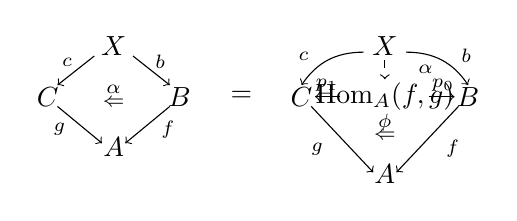
\begin{tikzpicture}[x=1.4em,y=1.4em]
  \node (x) at (0,2.6) {$X$};
  \node (c) at (-1.7,1.3) {$C$};
  \node (b) at (1.7,1.3) {$B$};
  \node (a) at (0,0) {$A$};
  \draw[->] (-0.5,2.35) -- (-1.45,1.6);
  \node at (-1.2,2.2) {$\scriptstyle c$};
  \draw[->] (0.5,2.35) -- (1.45,1.6);
  \node at (1.2,2.2) {$\scriptstyle b$};
  \node at (0,1.5) {$\scriptstyle\alpha$};
  \node at (0,1.14) {$\scriptstyle\Leftarrow$};
  \draw[->] (-1.45,1.05) -- (-0.3,0.1);
  \node at (-1.4,0.45) {$\scriptstyle g$};
  \draw[->] (1.45,1.05) -- (0.3,0.1);
  \node at (1.4,0.45) {$\scriptstyle f$};
  \node at (3.3,1.3) {$=$};
  \begin{scope}[shift={(7.0,0)}]
  \node (x) at (0,2.6) {$X$};
  \node (hom) at (0,1.3) {$\mathrm{Hom}_A(f,g)$};
  \draw[->,dashed] (0,2.25) -- (0,1.75);
  \node at (1.05,2.0) {$\scriptstyle\qcor{\alpha}$};
  \draw[->] (-0.55,2.45) to[bend right=28] (-2.15,1.6);
  \node at (-2.1,2.35) {$\scriptstyle c$};
  \draw[->] (0.55,2.45) to[bend left=28] (2.15,1.6);
  \node at (2.1,2.35) {$\scriptstyle b$};
  \node (c) at (-2.15,1.3) {$C$};
  \node (b) at (2.15,1.3) {$B$};
  \draw[->] (-1.15,1.3) -- (-1.8,1.3);
  \node at (-1.5,1.6) {$\scriptstyle p_{1}$};
  \draw[->] (1.15,1.3) -- (1.8,1.3);
  \node at (1.5,1.6) {$\scriptstyle p_{0}$};
  \node at (0,0.62) {$\scriptstyle\phi$};
  \node at (0,0.3) {$\scriptstyle\Leftarrow$};
  \node (a) at (0,-0.7) {$A$};
  \draw[->] (-1.9,1.05) -- (-0.3,-0.65);
  \node at (-1.75,-0.05) {$\scriptstyle g$};
  \draw[->] (1.9,1.05) -- (0.3,-0.65);
  \node at (1.75,-0.05) {$\scriptstyle f$};
  \end{scope}
\end{tikzpicture}
\end{center}
则存在\trFunctor{} $\qcor{\alpha}\colon X\to\mathrm{Hom}_A(f,g)$，使得 $b=p_{0}\qcor{\alpha}$、%
$c=p_{1}\qcor{\alpha}$，且 $\alpha=\phi\qcor{\alpha}$。
\item \textbf{\trTwoCellInduction{}：}给定\trFunctor{} $a,a'\colon X\to\mathrm{Hom}_A(f,g)$%
与\trNaturalTransformation{} $\tau_{1}$、$\tau_{0}$，使得
\begin{center}
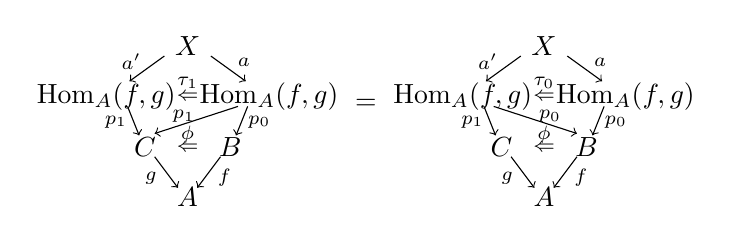
\begin{tikzpicture}[x=1.4em,y=1.4em]
  \node (x) at (0,2.8) {$X$};
  \node (hl) at (-2.1,1.5) {$\mathrm{Hom}_A(f,g)$};
  \node (hr) at (2.1,1.5) {$\mathrm{Hom}_A(f,g)$};
  \draw[->] (-0.6,2.55) -- (-1.5,1.9);
  \node at (-1.45,2.4) {$\scriptstyle a'$};
  \draw[->] (0.6,2.55) -- (1.5,1.9);
  \node at (1.45,2.4) {$\scriptstyle a$};
  \node at (0,1.85) {$\scriptstyle\tau_{1}$};
  \node at (0,1.5) {$\scriptstyle\Leftarrow$};
  \node (c) at (-1.1,0.2) {$C$};
  \node (b) at (1.1,0.2) {$B$};
  \draw[->] (-1.55,1.25) -- (-1.25,0.5);
  \node at (-1.85,0.85) {$\scriptstyle p_{1}$};
  \draw[->] (1.55,1.25) -- (1.25,0.5);
  \node at (1.85,0.85) {$\scriptstyle p_{0}$};
  \draw[->] (1.3,1.25) -- (-0.85,0.55);
  \node at (-0.1,1.0) {$\scriptstyle p_{1}$};
  \node at (0,0.52) {$\scriptstyle\phi$};
  \node at (0,0.18) {$\scriptstyle\Leftarrow$};
  \node (a2) at (0,-1.1) {$A$};
  \draw[->] (-0.85,-0.05) -- (-0.25,-0.85);
  \node at (-0.95,-0.6) {$\scriptstyle g$};
  \draw[->] (0.85,-0.05) -- (0.25,-0.85);
  \node at (0.95,-0.6) {$\scriptstyle f$};
  \node at (4.6,1.3) {$=$};
  \begin{scope}[shift={(9.2,0)}]
  \node (x) at (0,2.8) {$X$};
  \node (hl) at (-2.1,1.5) {$\mathrm{Hom}_A(f,g)$};
  \node (hr) at (2.1,1.5) {$\mathrm{Hom}_A(f,g)$};
  \draw[->] (-0.6,2.55) -- (-1.5,1.9);
  \node at (-1.45,2.4) {$\scriptstyle a'$};
  \draw[->] (0.6,2.55) -- (1.5,1.9);
  \node at (1.45,2.4) {$\scriptstyle a$};
  \node at (0,1.85) {$\scriptstyle\tau_{0}$};
  \node at (0,1.5) {$\scriptstyle\Leftarrow$};
  \node (c) at (-1.1,0.2) {$C$};
  \node (b) at (1.1,0.2) {$B$};
  \draw[->] (-1.55,1.25) -- (-1.25,0.5);
  \node at (-1.85,0.85) {$\scriptstyle p_{1}$};
  \draw[->] (1.55,1.25) -- (1.25,0.5);
  \node at (1.85,0.85) {$\scriptstyle p_{0}$};
  \draw[->] (-1.3,1.25) -- (0.85,0.55);
  \node at (0.15,1.0) {$\scriptstyle p_{0}$};
  \node at (0,0.52) {$\scriptstyle\phi$};
  \node at (0,0.18) {$\scriptstyle\Leftarrow$};
  \node (a2) at (0,-1.1) {$A$};
  \draw[->] (-0.85,-0.05) -- (-0.25,-0.85);
  \node at (-0.95,-0.6) {$\scriptstyle g$};
  \draw[->] (0.85,-0.05) -- (0.25,-0.85);
  \node at (0.95,-0.6) {$\scriptstyle f$};
  \end{scope}
\end{tikzpicture}
\end{center}
则存在\trNaturalTransformation{} $\tau\colon a\Rightarrow a'$，使得 $p_{1}\tau=\tau_{1}$%
且 $p_{0}\tau=\tau_{0}$。
\item \textbf{\trTwoCellConservativity{}：}对任何
\begin{center}
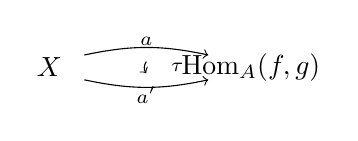
\begin{tikzpicture}[x=1.4em,y=1.4em]
  \node (x) at (0,0) {$X$};
  \node (h) at (5.2,0) {$\mathrm{Hom}_A(f,g)$};
  \draw[->] (0.9,0.32) to[bend left=12] (4.1,0.32);
  \node at (2.5,0.68) {$\scriptstyle a$};
  \draw[->] (0.9,-0.32) to[bend right=12] (4.1,-0.32);
  \node at (2.5,-0.72) {$\scriptstyle a'$};
  \draw[->] (2.5,0.15) to[bend right=35] (2.5,-0.15);
  \node at (3.3,0.0) {$\scriptstyle\tau$};
\end{tikzpicture}
\end{center}
若 $p_{1}\tau$ 与 $p_{0}\tau$ 皆为\trIsomorphism{}，则 $\tau$ 是\trIsomorphism{}。
\end{enumerate}
\end{proposition}

\begin{proof}
\trCosmologicalFunctor{} $\mathrm{Fun}(X,-)\colon\mathcal{K}\to\QCat$ 把\trPullback{}%
\eqref{eq:comma-pullback} 带为\trQuasiCategory{}的如下\trPullback
\begin{center}
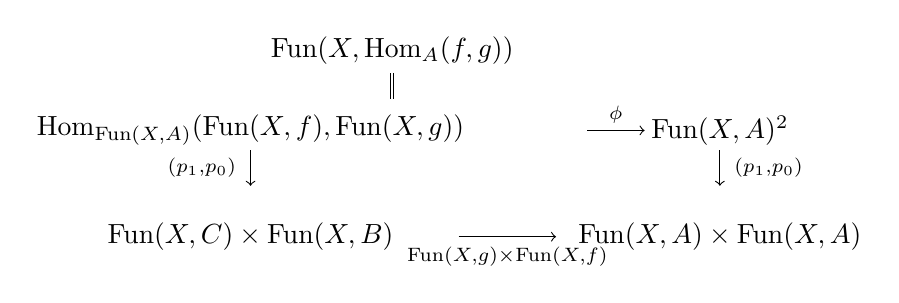
\begin{tikzpicture}[x=1.6em,y=1.6em]
  \node (top) at (3.2,3.2) {$\mathrm{Fun}(X,\mathrm{Hom}_A(f,g))$};
  \draw[double] (3.2,2.7) -- (3.2,2.1);
  \node (ml) at (0,1.4) {$\mathrm{Hom}_{\mathrm{Fun}(X,A)}(\mathrm{Fun}(X,f),\mathrm{Fun}(X,g))$};
  \node (mr) at (10.6,1.4) {$\mathrm{Fun}(X,A)^{2}$};
  \draw[->] (7.6,1.4) -- (8.9,1.4);
  \node at (8.25,1.76) {$\scriptstyle\phi$};
  \draw[->] (0,0.95) -- (0,0.15);
  \node at (-1.1,0.55) {$\scriptstyle(p_{1},p_{0})$};
  \node at (0.48,0.68) {$\scriptstyle\lrcorner$};
  \draw[->] (10.6,0.95) -- (10.6,0.15);
  \node at (11.7,0.55) {$\scriptstyle(p_{1},p_{0})$};
  \node (bl) at (0,-1.0) {$\mathrm{Fun}(X,C)\times\mathrm{Fun}(X,B)$};
  \node (br) at (10.6,-1.0) {$\mathrm{Fun}(X,A)\times\mathrm{Fun}(X,A)$};
  \draw[->] (4.7,-1.0) -- (6.9,-1.0);
  \node at (5.8,-1.44) {$\scriptstyle\mathrm{Fun}(X,g)\times\mathrm{Fun}(X,f)$};
\end{tikzpicture}
\end{center}
如今引理 3.1.7 表明：典范 2-\trCell{} \eqref{eq:comma-cone} 诱导出\trHomCategory{}之间的%
一个自然映射
\begin{center}
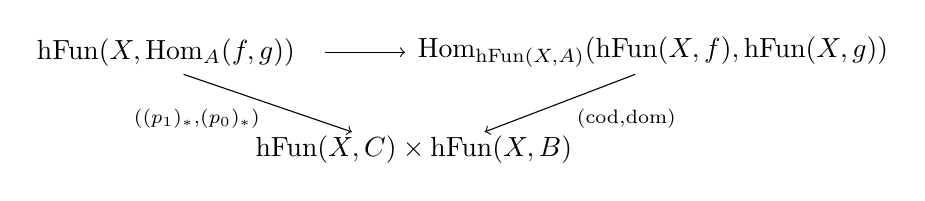
\begin{tikzpicture}[x=1.6em,y=1.6em]
  \node (tl) at (0,1.3) {$\mathrm{hFun}(X,\mathrm{Hom}_A(f,g))$};
  \node (tr) at (11.0,1.3) {$\mathrm{Hom}_{\mathrm{hFun}(X,A)}(\mathrm{hFun}(X,f),\mathrm{hFun}(X,g))$};
  \draw[->] (3.6,1.3) -- (5.4,1.3);
  \node (bm) at (5.6,-0.9) {$\mathrm{hFun}(X,C)\times\mathrm{hFun}(X,B)$};
  \draw[->] (0.4,0.8) -- (4.2,-0.5);
  \node at (0.7,-0.2) {$\scriptstyle((p_{1})_{*},(p_{0})_{*})$};
  \draw[->] (10.6,0.8) -- (7.2,-0.5);
  \node at (10.4,-0.2) {$\scriptstyle(\mathrm{cod},\mathrm{dom})$};
\end{tikzpicture}
\end{center}
它居于 $\mathrm{hFun}(X,C\times B)\cong\mathrm{hFun}(X,C)\times\mathrm{hFun}(X,B)$ 之上，%
是一个\trSmotheringFunctor{}。\trOneCellInduction{}、\trTwoCellInduction{}与%
\trTwoCellConservativity{}诸性质，分别由这一\trSmotheringFunctor{}的对象上的满射性、%
满性与保守性得证。
\end{proof}

由一个固定的\trNaturalTransformation{} $\alpha\colon fb\Rightarrow gc$ 所诱导的诸%
\trFunctor{} $\qcor{\alpha}\colon X\to\mathrm{Hom}_A(f,g)$，在 $C\times B$ 之上直至%
\trFiberedIsomorphism{}唯一。

\begin{proposition}\label{prop:whiskering-comma-bijection}
与\trCommaCone \eqref{eq:comma-cone} 作\trWhiskering{}，在下示左侧的诸\trNaturalTransformation{}%
与下示右侧的、从 $C$ 到 $B$ 的诸\trSpan{}映射的\trFiberedIsomorphism{}类之间，诱导出%
一个双射：
\[
\left\{\vcenter{\hbox{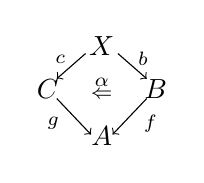
\begin{tikzpicture}[x=1.3em,y=1.3em]
  \node (x) at (0,2.2) {$X$};
  \node (c) at (-1.5,1.0) {$C$};
  \node (b) at (1.5,1.0) {$B$};
  \node (a) at (0,-0.3) {$A$};
  \draw[->] (-0.45,2.0) -- (-1.25,1.3);
  \node at (-1.15,1.85) {$\scriptstyle c$};
  \draw[->] (0.45,2.0) -- (1.25,1.3);
  \node at (1.15,1.85) {$\scriptstyle b$};
  \node at (0,1.2) {$\scriptstyle\alpha$};
  \node at (0,0.86) {$\scriptstyle\Leftarrow$};
  \draw[->] (-1.25,0.75) -- (-0.3,-0.25);
  \node at (-1.35,0.05) {$\scriptstyle g$};
  \draw[->] (1.25,0.75) -- (0.3,-0.25);
  \node at (1.35,0.05) {$\scriptstyle f$};
\end{tikzpicture}}}\right\}
\;\longleftrightarrow\;
\left\{\vcenter{\hbox{\begin{tikzpicture}[x=1.3em,y=1.3em]
  \node (x) at (0,2.6) {$X$};
  \node (c) at (-2.0,1.4) {$C$};
  \node (b) at (2.0,1.4) {$B$};
  \draw[->] (-0.5,2.4) -- (-1.6,1.7);
  \node at (-1.45,2.25) {$\scriptstyle c$};
  \draw[->] (0.5,2.4) -- (1.6,1.7);
  \node at (1.45,2.25) {$\scriptstyle b$};
  \draw[->] (0,2.25) -- (0,0.1);
  \node at (0.85,1.2) {$\scriptstyle\qcor{\alpha}$};
  \node (hom) at (0,-0.5) {$\mathrm{Hom}_A(f,g)$};
  \draw[->] (-0.75,-0.75) -- (-1.8,1.15);
  \node at (-1.95,0.3) {$\scriptstyle p_{1}$};
  \draw[->] (0.75,-0.75) -- (1.8,1.15);
  \node at (1.95,0.3) {$\scriptstyle p_{0}$};
\end{tikzpicture}}}\right\}_{/\cong}
\]
其中诸\trFiberedIsomorphism{}由\trInvertible{} 2-\trCell
\begin{center}
\begin{tikzpicture}[x=1.4em,y=1.4em]
  \node (x) at (0,2.4) {$X$};
  \node (c) at (-3.2,1.2) {$C$};
  \node (b) at (3.2,1.2) {$B$};
  \draw[->] (-0.55,2.2) -- (-2.7,1.45);
  \node at (-2.1,2.05) {$\scriptstyle c$};
  \draw[->] (0.55,2.2) -- (2.7,1.45);
  \node at (2.1,2.05) {$\scriptstyle b$};
  \draw[->] (-0.3,2.05) to[bend right=10] (-0.7,-0.6);
  \node at (-1.25,0.8) {$\scriptstyle\qcor{\alpha'}$};
  \draw[->] (0.3,2.05) to[bend left=10] (0.7,-0.6);
  \node at (1.25,0.8) {$\scriptstyle\qcor{\alpha}$};
  \draw[->] (-0.12,0.9) to[bend right=30] (0.48,0.62);
  \node at (0.85,1.1) {$\scriptstyle\gamma$};
  \node at (0.2,0.42) {$\scriptstyle\simeq$};
  \node (hom) at (0,-1.5) {$\mathrm{Hom}_A(f,g)$};
  \draw[->] (-0.6,-1.75) -- (-2.85,0.95);
  \node at (-2.7,-0.6) {$\scriptstyle p_{1}$};
  \draw[->] (0.6,-1.75) -- (2.85,0.95);
  \node at (2.7,-0.6) {$\scriptstyle p_{0}$};
\end{tikzpicture}
\end{center}
给出，满足 $p_{1}\gamma=\mathrm{id}_{c}$ 且 $p_{0}\gamma=\mathrm{id}_{b}$。
\end{proposition}

\begin{proof}
引理 3.1.3 证明了\cref{prop:comma-weak-universal-property}的\trSmotheringFunctor{}之%
诸\trFiber{}皆为连通\trGroupoid{}。$\alpha$ 之上的\trFiber{}，其对象是与\trCommaCone $\phi$ 作%
\trWhiskering{}后给出 $\alpha$ 的那些\trFunctor{} $X\to\mathrm{Hom}_A(f,g)$，其态射是与%
$(p_{1},p_{0})\colon\mathrm{Hom}_A(f,g)\twoheadrightarrow C\times B$ 作\trWhiskering{}后%
成为恒同 2-\trCell{} $(\mathrm{id}_{c},\mathrm{id}_{b})$ 的那些\trInvertible{}%
2-\trCell{}。\trSmotheringFunctor{}的作用在其余域的对象与各自的\trFiber{}之间定义了%
一个双射。
\end{proof}

\trHomotopyTwoCategory{}中\trCospan{}的反松弛映射同样诱导\trCommaInfinityCategory{}%
之间的映射：

\begin{observation}\label{obs:oplax-cospan-maps}
由\trOneCellInduction{}，\trDiagram
\begin{center}
\begin{tikzpicture}[x=1.7em,y=1.7em]
  \node (c) at (0,1.3) {$C$};
  \node (a) at (3.4,1.3) {$A$};
  \node (b) at (6.8,1.3) {$B$};
  \node (cb) at (0,0) {$\bar{C}$};
  \node (ab) at (3.4,0) {$\bar{A}$};
  \node (bb) at (6.8,0) {$\bar{B}$};
  \draw[->] (0.5,1.3) -- (2.9,1.3);
  \node at (1.7,1.66) {$\scriptstyle g$};
  \draw[->] (6.3,1.3) -- (3.9,1.3);
  \node at (5.1,1.66) {$\scriptstyle f$};
  \draw[->] (0.5,0) -- (2.9,0);
  \node at (1.7,-0.36) {$\scriptstyle\bar{g}$};
  \draw[->] (6.3,0) -- (3.9,0);
  \node at (5.1,-0.36) {$\scriptstyle\bar{f}$};
  \draw[->] (0,0.95) -- (0,0.35);
  \node at (-0.44,0.65) {$\scriptstyle r$};
  \draw[->] (3.4,0.95) -- (3.4,0.35);
  \node at (3.84,0.65) {$\scriptstyle p$};
  \draw[->] (6.8,0.95) -- (6.8,0.35);
  \node at (7.24,0.65) {$\scriptstyle q$};
  \node at (1.7,0.68) {$\scriptstyle\Downarrow$};
  \node at (2.2,0.68) {$\scriptstyle\gamma$};
  \node at (5.1,0.68) {$\scriptstyle\Downarrow$};
  \node at (5.6,0.68) {$\scriptstyle\beta$};
\end{tikzpicture}
\end{center}
诱导出如下图右所示、\trCommaInfinityCategory{}之间的一个映射：
\begin{center}
\begin{tikzpicture}[x=1.5em,y=1.5em]
  \node (hom) at (0,4.4) {$\mathrm{Hom}_A(f,g)$};
  \node (c) at (-2.4,3.0) {$C$};
  \node (b) at (2.4,3.0) {$B$};
  \draw[->] (-1.0,4.15) -- (-2.05,3.3);
  \node at (-1.95,3.9) {$\scriptstyle p_{1}$};
  \draw[->] (1.0,4.15) -- (2.05,3.3);
  \node at (1.95,3.9) {$\scriptstyle p_{0}$};
  \node at (0,3.22) {$\scriptstyle\phi$};
  \node at (0,2.88) {$\scriptstyle\Leftarrow$};
  \draw[->] (-2.4,2.65) -- (-2.4,1.75);
  \node at (-2.85,2.2) {$\scriptstyle r$};
  \draw[->] (2.4,2.65) -- (2.4,1.75);
  \node at (2.85,2.2) {$\scriptstyle q$};
  \draw[->] (-2.15,2.75) -- (-0.5,1.55);
  \node at (-1.8,2.3) {$\scriptstyle g$};
  \draw[->] (2.15,2.75) -- (0.5,1.55);
  \node at (1.8,2.3) {$\scriptstyle f$};
  \node (ab) at (0,1.4) {$A$};
  \node (cb) at (-2.4,1.4) {$\bar{C}$};
  \node (bb) at (2.4,1.4) {$\bar{B}$};
  \node at (-1.2,1.72) {$\scriptstyle\gamma$};
  \node at (-1.2,1.38) {$\scriptstyle\Leftarrow$};
  \node at (1.2,1.72) {$\scriptstyle\beta$};
  \node at (1.2,1.38) {$\scriptstyle\Leftarrow$};
  \draw[->] (0,1.05) -- (0,0.15);
  \node at (0.5,0.6) {$\scriptstyle p$};
  \node (abbar) at (0,-0.5) {$\bar{A}$};
  \draw[->] (-2.15,1.15) -- (-0.45,-0.45);
  \node at (-1.9,-0.05) {$\scriptstyle\bar{g}$};
  \draw[->] (2.15,1.15) -- (0.45,-0.45);
  \node at (1.9,-0.05) {$\scriptstyle\bar{f}$};
  \node at (4.4,2.0) {$=$};
  \begin{scope}[shift={(8.8,0)}]
  \node (hom) at (0,4.4) {$\mathrm{Hom}_A(f,g)$};
  \node (homb) at (0,2.8) {$\mathrm{Hom}_{\bar{A}}(\bar{f},\bar{g})$};
  \draw[->,dotted] (0,4.05) -- (0,3.4);
  \node at (1.35,3.75) {$\scriptstyle\beta\downarrow\gamma$};
  \draw[->] (-0.9,4.15) to[bend right=22] (-2.5,1.7);
  \node at (-3.1,3.3) {$\scriptstyle rp_{1}$};
  \draw[->] (0.9,4.15) to[bend left=22] (2.5,1.7);
  \node at (3.1,3.3) {$\scriptstyle qp_{0}$};
  \node (cb) at (-2.4,1.4) {$\bar{C}$};
  \node (bb) at (2.4,1.4) {$\bar{B}$};
  \draw[->] (-1.0,2.55) -- (-1.95,1.7);
  \node at (-1.8,2.25) {$\scriptstyle p_{1}$};
  \draw[->] (1.0,2.55) -- (1.95,1.7);
  \node at (1.8,2.25) {$\scriptstyle p_{0}$};
  \node at (0,1.72) {$\scriptstyle\phi$};
  \node at (0,1.38) {$\scriptstyle\Leftarrow$};
  \node (abbar) at (0,-0.5) {$\bar{A}$};
  \draw[->] (-2.15,1.15) -- (-0.45,-0.45);
  \node at (-1.9,-0.05) {$\scriptstyle\bar{g}$};
  \draw[->] (2.15,1.15) -- (0.45,-0.45);
  \node at (1.9,-0.05) {$\scriptstyle\bar{f}$};
  \end{scope}
\end{tikzpicture}
\end{center}
它在直至\trFiberedIsomorphism{}的意义下良定且函子（见%
\cref{ex:oplax-functoriality}）。
\end{observation}

\trCommaInfinityCategory{}的诸多用途之一，是定义一个\trInfinityCategory{} $A$ 的%
两个\trElement{}之间的内部\trMappingSpace{}。这正是我们采用记号「$\mathrm{Hom}_A$」的动机之一。

\begin{definition}[\trMappingSpace]\label{def:mapping-space}
\trInfinityCategory{} $A$ 的两个\trElement{} $x,y\colon\qcOne\to A$ 之间的%
\textbf{\trMappingSpace}（mapping space），是由如下拉回\trDiagram{}所定义的%
\trCommaInfinityCategory{} $\mathrm{Hom}_A(x,y)$
\begin{center}
\begin{tikzpicture}[x=1.6em,y=1.6em]
  \node (tl) at (0,1.4) {$\mathrm{Hom}_A(x,y)$};
  \node (tr) at (4.4,1.4) {$A^{2}$};
  \node (bl) at (0,0) {$\qcOne$};
  \node (br) at (4.4,0) {$A\times A$};
  \draw[->] (1.9,1.4) -- (3.4,1.4);
  \node at (2.65,1.78) {$\scriptstyle\qcor{\phi}$};
  \draw[->] (0,1.05) -- (0,0.35);
  \node at (-1.1,0.7) {$\scriptstyle(p_{1},p_{0})$};
  \node at (0.48,0.78) {$\scriptstyle\lrcorner$};
  \draw[->] (4.4,1.05) -- (4.4,0.35);
  \node at (5.5,0.7) {$\scriptstyle(p_{1},p_{0})$};
  \draw[->] (0.6,0) -- (3.2,0);
  \node at (1.9,-0.38) {$\scriptstyle(y,x)$};
\end{tikzpicture}
\end{center}
\end{definition}

\trMappingSpace{}在定义 1.2.26 的意义下是\trDiscrete{}：

\begin{proposition}[\trMappingSpace{}是离散的]\label{prop:mapping-spaces-discrete}
对\trInfinityCategory{} $A$ 的任意一对\trElement{} $x,y\colon\qcOne\to A$，\trMappingSpace%
$\mathrm{Hom}_A(x,y)$ 是\trDiscrete{}。
\end{proposition}

\begin{proof}
我们必须证明：对任意\trInfinityCategory{} $X$，\trFunctorSpace{}%
$\mathrm{Fun}(X,\mathrm{Hom}_A(x,y))$ 是一个\trKanComplex{}。这恰好当%
$\mathrm{hFun}(X,\mathrm{Hom}_A(x,y))$ 是一个\trGroupoid{}时成立——也就是说，余定义域为%
$\mathrm{Hom}_A(x,y)$ 的任何 2-\trCell{}都是\trInvertible{}。由\trTwoCellConservativity{}，%
余定义域为 $\mathrm{Hom}_A(x,y)$ 的一个 2-\trCell{}是\trInvertible{}，恰好当它与%
\trIsofibration{} $(p_{1},p_{0})\colon\mathrm{Hom}_A(x,y)\twoheadrightarrow\qcOne\times\qcOne$%
的\trWhiskering{}复合是一条\trInvertible{} 2-\trCell{}；而事实上，由于 $\qcOne$ 是%
\trTwoTerminalObject{}，这一\trWhiskering{}复合是恒同。
\end{proof}

\cref{prop:comma-weak-universal-property}的弱\trUniversalProperty{}在 $C\times B$ 之上%
直至\trFiberedEquivalence{}（见\cref{def:fibered-equivalence}）刻画了诸\trCommaInfinityCategory{}。

\begin{proposition}[逗号∞-范畴的唯一性]\label{prop:comma-uniqueness}
对任何\trFiberedEquivalence{}于 $\mathrm{Hom}_A(f,g)\twoheadrightarrow C\times B$ 的%
\trIsofibration{} $(e_{1},e_{0})\colon E\twoheadrightarrow C\times B$，由\trEquivalence{}%
$e\colon E\rightleftarrows\mathrm{Hom}_A(f,g)$ 所编码的 2-\trCell
\begin{center}
\begin{tikzpicture}[x=1.5em,y=1.5em]
  \node (e) at (0,2.0) {$E$};
  \node (c) at (-1.8,0.8) {$C$};
  \node (b) at (1.8,0.8) {$B$};
  \node (a) at (0,-0.5) {$A$};
  \draw[->] (-0.7,1.75) -- (-1.55,1.05);
  \node at (-1.6,1.55) {$\scriptstyle e_{1}$};
  \draw[->] (0.7,1.75) -- (1.55,1.05);
  \node at (1.6,1.55) {$\scriptstyle e_{0}$};
  \node at (0,1.0) {$\scriptstyle\epsilon$};
  \node at (0,0.66) {$\scriptstyle\Leftarrow$};
  \draw[->] (-1.55,0.55) -- (-0.35,-0.45);
  \node at (-1.5,0.0) {$\scriptstyle g$};
  \draw[->] (1.55,0.55) -- (0.35,-0.45);
  \node at (1.5,0.0) {$\scriptstyle f$};
\end{tikzpicture}
\end{center}
满足\cref{prop:comma-weak-universal-property}的弱\trUniversalProperty{}。反之，若%
$(d_{1},d_{0})\colon D\twoheadrightarrow C\times B$ 与 $(e_{1},e_{0})\colon E\twoheadrightarrow C\times B$%
配备有 2-\trCell
\begin{rveq}\label{eq:comma-uniqueness-cells}
\begin{tikzpicture}[x=1.5em,y=1.5em,baseline=(current bounding box.center)]
  \node (d) at (0,1.6) {$D$};
  \node (c) at (-1.8,0.4) {$C$};
  \node (b) at (1.8,0.4) {$B$};
  \node (a) at (0,-0.9) {$A$};
  \draw[->] (-0.7,1.35) -- (-1.55,0.65);
  \node at (-1.6,1.15) {$\scriptstyle d_{1}$};
  \draw[->] (0.7,1.35) -- (1.55,0.65);
  \node at (1.6,1.15) {$\scriptstyle d_{0}$};
  \node at (0,0.6) {$\scriptstyle\delta$};
  \node at (0,0.26) {$\scriptstyle\Leftarrow$};
  \draw[->] (-1.55,0.15) -- (-0.35,-0.85);
  \node at (-1.5,-0.5) {$\scriptstyle g$};
  \draw[->] (1.55,0.15) -- (0.35,-0.85);
  \node at (1.5,-0.5) {$\scriptstyle f$};
  \node at (4.0,0.4) {与};
  \begin{scope}[shift={(8.0,0)}]
  \node (e) at (0,1.6) {$E$};
  \node (c) at (-1.8,0.4) {$C$};
  \node (b) at (1.8,0.4) {$B$};
  \node (a) at (0,-0.9) {$A$};
  \draw[->] (-0.7,1.35) -- (-1.55,0.65);
  \node at (-1.6,1.15) {$\scriptstyle e_{1}$};
  \draw[->] (0.7,1.35) -- (1.55,0.65);
  \node at (1.6,1.15) {$\scriptstyle e_{0}$};
  \node at (0,0.6) {$\scriptstyle\epsilon$};
  \node at (0,0.26) {$\scriptstyle\Leftarrow$};
  \draw[->] (-1.55,0.15) -- (-0.35,-0.85);
  \node at (-1.5,-0.5) {$\scriptstyle g$};
  \draw[->] (1.55,0.15) -- (0.35,-0.85);
  \node at (1.5,-0.5) {$\scriptstyle f$};
  \end{scope}
\end{tikzpicture}
\end{rveq}
且它们满足\cref{prop:comma-weak-universal-property}的弱\trUniversalProperty{}，则%
$D\simeq_{C\times B}E$。
\end{proposition}

\begin{proof}
第一陈述的证明完全照搬\cref{prop:arrow-category-uniqueness}这一特殊情形的做法。我们证明逆方向，%
亦即给出练习 3.2.ii 的解。
考察满足\cref{prop:comma-weak-universal-property}所列诸弱\trUniversalProperty{}的%
一对 2-\trCell{} \eqref{eq:comma-uniqueness-cells}。\trOneCellInduction{}供给出%
一个\trSpan{}映射
\begin{center}
\begin{tikzpicture}[x=1.4em,y=1.4em]
  \node (d) at (0,1.8) {$D$};
  \node (c) at (-1.9,0.6) {$C$};
  \node (b) at (1.9,0.6) {$B$};
  \node (a) at (0,-0.7) {$A$};
  \draw[->] (-0.7,1.55) -- (-1.6,0.85);
  \node at (-1.7,1.35) {$\scriptstyle d_{1}$};
  \draw[->] (0.7,1.55) -- (1.6,0.85);
  \node at (1.7,1.35) {$\scriptstyle d_{0}$};
  \node at (0,0.8) {$\scriptstyle\delta$};
  \node at (0,0.46) {$\scriptstyle\Leftarrow$};
  \draw[->] (-1.6,0.35) -- (-0.35,-0.65);
  \node at (-1.55,-0.3) {$\scriptstyle g$};
  \draw[->] (1.6,0.35) -- (0.35,-0.65);
  \node at (1.55,-0.3) {$\scriptstyle f$};
  \node at (3.5,0.6) {$=$};
  \begin{scope}[shift={(6.8,0.8)}]
  \node (d) at (0,2.0) {$D$};
  \node (e) at (0,0.7) {$E$};
  \draw[->,dashed] (0,1.65) -- (0,1.15);
  \node at (0.9,1.4) {$\scriptstyle\qcor{\epsilon}$};
  \draw[->] (-0.55,1.85) to[bend right=25] (-2.05,0.95);
  \node at (-2.15,1.75) {$\scriptstyle d_{1}$};
  \draw[->] (0.55,1.85) to[bend left=25] (2.05,0.95);
  \node at (2.15,1.75) {$\scriptstyle d_{0}$};
  \node (c) at (-2.05,0.6) {$C$};
  \node (b) at (2.05,0.6) {$B$};
  \draw[->] (-0.85,0.45) -- (-1.65,-0.05);
  \node at (-1.6,0.5) {$\scriptstyle e_{1}$};
  \draw[->] (0.85,0.45) -- (1.65,-0.05);
  \node at (1.6,0.5) {$\scriptstyle e_{0}$};
  \node at (0,-0.1) {$\scriptstyle\epsilon$};
  \node at (0,-0.44) {$\scriptstyle\Leftarrow$};
  \node (a) at (0,-1.5) {$A$};
  \draw[->] (-1.8,0.35) -- (-0.35,-1.45);
  \node at (-1.65,-0.85) {$\scriptstyle g$};
  \draw[->] (1.8,0.35) -- (0.35,-1.45);
  \node at (1.65,-0.85) {$\scriptstyle f$};
  \end{scope}
\end{tikzpicture}
\end{center}
交换 $\delta$ 与 $\epsilon$ 的角色，便得到第二个\trSpan{}映射 $\qcor{\epsilon}\colon E\to D$，%
它具有性质 $\epsilon\qcor{\delta}\qcor{\epsilon}=\epsilon$ 与 $\delta\qcor{\epsilon}\qcor{\delta}=\delta$。%
\footnote{原书印作「$\epsilon'\qcor{\delta}\qcor{\epsilon}=\epsilon$」，其中 $\epsilon'$ 无定义，%
疑为「$\epsilon$」之误，此处径改。——译者注}%
由\cref{prop:whiskering-comma-bijection}可得：在 $C\times B$ 上%
$\qcor{\delta}\qcor{\epsilon}\cong\mathrm{id}_{E}$，在 $C\times B$ 上%
$\qcor{\epsilon}\qcor{\delta}\cong\mathrm{id}_{D}$。这就定义了一条\trFiberedEquivalence{}%
$D\simeq E$ 的数据。\footnote{正如警告 3.2.9 所暗示的那样，编码一条%
\trFiberedEquivalence{}的 2-范畴论数据存在一点轻微的含混。命题 3.6.4 为补全%
这一证明提供了一个小的助推。}
\end{proof}

沿我们处理\trArrowInfinityCategory{}时的同一约定，把「\trCommaInfinityCategory」%
这一称谓从\cref{def:comma-infinity-category}所构造的严格模型扩充到任何纤维化等价于%
它的\trInfinityCategory{}、并把其伴随的 2-\trCell{}称为「\trCommaCone」，是便利之举。例如，%
在 4.2 节中，我们将为一个由固定单纯集索引的\trDiagram{}之\trInfinityCategoryOfCones{}引入多个模型，%
它们在发展\trLimit{}的\trUniversalProperty{}的种种等价表述时很有用。

\subsection*{练习}

\begin{exercise}[命题 C.1.12]\label{ex:hom-p-factors}
通过观察 $\mathrm{Hom}_p(q,r)$ 分解为「$\partial\Delta[1]\hookrightarrow\Delta[1]$ 与 $p$ 的%
\trLeibnizCotensor」的一个\trPullback{}、再接上 $r\times q$ 的一个\trPullback{}来分解，%
完成\cref{prop:maps-between-commas}的证明。
\end{exercise}

\begin{exercise}\label{ex:oplax-functoriality}
利用\cref{prop:whiskering-comma-bijection}，为\cref{obs:oplax-cospan-maps}所描述的%
逗号构造在\trCospan{}的反松弛态射之下直至同构的函子性提供论证。
\end{exercise}

\begin{exercise}\label{ex:rectification}
\cref{ex:hom-p-factors}与\cref{ex:oplax-functoriality}例示了%
\trCommaInfinityCategory{}构造的严格单纯\trUniversalProperty{}与\trBicategory%
\trUniversalProperty{}各自的相对优点与缺点：前者给出一个严格函子的作用，却只对%
严格交换的\trCospan{}映射如此；后者给出\trCospan{}的反松弛变换的一个作用，%
却直至同构才是函子的。在这两种构造之间居中调停，用引理 1.2.19 与命题 1.4.9 把%
一个拟交换\trDiagram
\begin{center}
\begin{tikzpicture}[x=1.7em,y=1.7em]
  \node (c) at (0,1.3) {$C$};
  \node (a) at (3.4,1.3) {$A$};
  \node (b) at (6.8,1.3) {$B$};
  \node (cb) at (0,0) {$\bar{C}$};
  \node (ab) at (3.4,0) {$\bar{A}$};
  \node (bb) at (6.8,0) {$\bar{B}$};
  \draw[->] (0.5,1.3) -- (2.9,1.3);
  \node at (1.7,1.66) {$\scriptstyle g$};
  \draw[->] (6.3,1.3) -- (3.9,1.3);
  \node at (5.1,1.66) {$\scriptstyle f$};
  \draw[->] (0.5,0) -- (2.9,0);
  \node at (1.7,-0.36) {$\scriptstyle\bar{g}$};
  \draw[->] (6.3,0) -- (3.9,0);
  \node at (5.1,-0.36) {$\scriptstyle\bar{f}$};
  \draw[->] (0,0.95) -- (0,0.35);
  \node at (-0.44,0.65) {$\scriptstyle r$};
  \draw[->] (3.4,0.95) -- (3.4,0.35);
  \node at (3.84,0.65) {$\scriptstyle p$};
  \draw[->] (6.8,0.95) -- (6.8,0.35);
  \node at (7.24,0.65) {$\scriptstyle q$};
  \node at (1.7,0.72) {$\scriptstyle\Downarrow$};
  \node at (2.2,0.88) {$\scriptstyle\gamma$};
  \node at (1.7,0.34) {$\scriptstyle\simeq$};
  \node at (5.1,0.72) {$\scriptstyle\Downarrow$};
  \node at (5.6,0.88) {$\scriptstyle\beta$};
  \node at (5.1,0.34) {$\scriptstyle\simeq$};
\end{tikzpicture}
\end{center}
\trRectify{}成一个与之等价的严格交换\trDiagram{}，并证明诱导映射 $\mathrm{Hom}_p(q,r)$ 等价于%
$\beta\downarrow\gamma$。
\end{exercise}

\begin{exercise}\label{ex:oplax-equivalence}
证明：由如下\trDiagram
\begin{center}
\begin{tikzpicture}[x=1.7em,y=1.7em]
  \node (c) at (0,1.3) {$C$};
  \node (a) at (3.4,1.3) {$A$};
  \node (b) at (6.8,1.3) {$B$};
  \node (cb) at (0,0) {$\bar{C}$};
  \node (ab) at (3.4,0) {$\bar{A}$};
  \node (bb) at (6.8,0) {$\bar{B}$};
  \draw[->] (0.5,1.3) -- (2.9,1.3);
  \node at (1.7,1.66) {$\scriptstyle g$};
  \draw[->] (6.3,1.3) -- (3.9,1.3);
  \node at (5.1,1.66) {$\scriptstyle f$};
  \draw[->] (0.5,0) -- (2.9,0);
  \node at (1.7,-0.36) {$\scriptstyle\bar{g}$};
  \draw[->] (6.3,0) -- (3.9,0);
  \node at (5.1,-0.36) {$\scriptstyle\bar{f}$};
  \draw[->] (0,0.95) -- (0,0.35);
  \node at (-0.44,0.65) {$\scriptstyle r$};
  \draw[->] (3.4,0.95) -- (3.4,0.35);
  \node at (3.84,0.65) {$\scriptstyle p$};
  \draw[->] (6.8,0.95) -- (6.8,0.35);
  \node at (7.24,0.65) {$\scriptstyle q$};
  \node at (1.7,0.72) {$\scriptstyle\Downarrow$};
  \node at (2.2,0.88) {$\scriptstyle\gamma$};
  \node at (1.7,0.34) {$\scriptstyle\simeq$};
  \node at (5.1,0.72) {$\scriptstyle\Downarrow$};
  \node at (5.6,0.88) {$\scriptstyle\beta$};
  \node at (5.1,0.34) {$\scriptstyle\simeq$};
\end{tikzpicture}
\end{center}
——其中 $\beta$ 与 $\gamma$ 是\trIsomorphism{}，而 $p$、$q$ 与 $r$ 是\trEquivalence{}——%
所诱导的\trCommaInfinityCategory{}之间的\trFunctor{}，在 $r\times q$ 之上定义了%
一个\trEquivalence
\begin{center}
\begin{tikzpicture}[x=1.7em,y=1.7em]
  \node (tl) at (0,1.4) {$\mathrm{Hom}_A(f,g)$};
  \node (tr) at (6.2,1.4) {$\mathrm{Hom}_{\bar{A}}(\bar{f},\bar{g})$};
  \node (bl) at (0,0) {$C\times B$};
  \node (br) at (6.2,0) {$\bar{C}\times\bar{B}$};
  \draw[->,dashed] (2.6,1.4) -- (3.7,1.4);
  \node at (3.15,1.96) {$\scriptstyle\beta\downarrow\gamma$};
  \node at (3.15,1.66) {$\scriptstyle\simeq$};
  \draw[->] (0,1.05) -- (0,0.35);
  \node at (-1.1,0.7) {$\scriptstyle(p_{1},p_{0})$};
  \draw[->] (6.2,1.05) -- (6.2,0.35);
  \node at (7.3,0.7) {$\scriptstyle(p_{1},p_{0})$};
  \draw[->] (1.3,0) -- (4.5,0);
  \node at (2.9,0.22) {$\scriptstyle\sim$};
  \node at (2.9,-0.38) {$\scriptstyle r\times q$};
\end{tikzpicture}
\end{center}
\end{exercise}
   %
\providecommand{\qcOne}{\mathbf{1}}   %
\providecommand{\qcor}[1]{\ulcorner#1\urcorner}   %

\section{可表示逗号∞-范畴}\label{sec:representable-comma-infinity-categories}

定义 3.4.1 为任何\trCospan{}构造了一个\trCommaInfinityCategory{}。%
在\trCospan{}的一条腿为恒同的特殊情形，这提供了两种对偶机制，把∞-范畴之间的一个%
\trFunctor{}编码为一个∞-范畴本身。

\begin{definition}[左表示与右表示]\label{def:left-right-representations}
任何\trFunctor{} $f\colon A\to B$ 都作为一个\trCommaInfinityCategory{}具有一个\textbf{左表示}%
（left representation）与一个\textbf{右表示}（right representation），如下左与下右所示：
\begin{center}
\begin{tikzpicture}[x=1.5em,y=1.5em]
  \node (hom) at (0,2.2) {$\mathrm{Hom}_B(f,B)$};
  \node (b) at (-2.0,0.8) {$B$};
  \node (a) at (2.0,0.8) {$A$};
  \draw[->] (-0.85,1.95) -- (-1.75,1.1);
  \node at (-1.8,1.75) {$\scriptstyle p_{1}$};
  \draw[->] (0.85,1.95) -- (1.75,1.1);
  \node at (1.8,1.75) {$\scriptstyle p_{0}$};
  \node at (0,1.02) {$\scriptstyle\phi$};
  \node at (0,0.64) {$\scriptstyle\Leftarrow$};
  \draw[->] (1.7,0.8) -- (-1.4,0.8);
  \node at (0.2,0.34) {$\scriptstyle f$};
  \node at (4.0,1.5) {\qquad};
  \begin{scope}[shift={(8.0,0)}]
  \node (hom) at (0,2.2) {$\mathrm{Hom}_B(B,f)$};
  \node (a) at (-2.0,0.8) {$A$};
  \node (b) at (2.0,0.8) {$B$};
  \draw[->] (-0.85,1.95) -- (-1.75,1.1);
  \node at (-1.8,1.75) {$\scriptstyle p_{1}$};
  \draw[->] (0.85,1.95) -- (1.75,1.1);
  \node at (1.8,1.75) {$\scriptstyle p_{0}$};
  \node at (0,1.02) {$\scriptstyle\phi$};
  \node at (0,0.64) {$\scriptstyle\Leftarrow$};
  \draw[->] (-1.7,0.8) -- (1.4,0.8);
  \node at (-0.2,0.34) {$\scriptstyle f$};
  \end{scope}
\end{tikzpicture}
\end{center}
\end{definition}

其中，为节省版面，我们把上左所示的 $f$ 的\textbf{左\trCommaCone{}}（left comma cone）%
与上右所示的 $f$ 的\textbf{右\trCommaCone{}}（right comma cone）画作居于三角形而非%
方形之中。

由命题 3.4.11，\trCommaCone{}的弱\trUniversalProperty{}把\textbf{逗号\trSpan}（comma span）%
在余定义域对象之积上直至\trFiberedEquivalence{}刻划。于是：

\begin{definition}\label{def:left-right-representable}
给定一个\trCospan{} $C\xrightarrow{\;g\;}A\xleftarrow{\;f\;}B$，若存在\trFunctor{}%
$\ell\colon B\to C$ 使得
\[
\mathrm{Hom}_A(f,g)\simeq_{C\times B}\mathrm{Hom}_C(\ell,C)
\]
则称\trCommaInfinityCategory{} $\mathrm{Hom}_A(f,g)\twoheadrightarrow C\times B$ 是\textbf{左可表示的}%
（left representable）；若存在\trFunctor{} $r\colon C\to B$ 使得
\[
\mathrm{Hom}_A(f,g)\simeq_{C\times B}\mathrm{Hom}_B(B,r)
\]
则称它是\textbf{右可表示的}（right representable）。%
\end{definition}

在本节中，我们证明一个可表示性定理：\trCommaInfinityCategory{} $\mathrm{Hom}_A(f,g)$ 是右可表示的，%
当且仅当 $g\colon C\to A$ 沿 $f\colon B\to A$ 具有一个\textbf{绝对右提升}%
（absolute right lifting），此时表示\trFunctor{} $r\colon C\to B$ 即定义出所断言的\trLifting{}。%
我们用三则定理来证明这一结果，每一则都强化前一则的陈述。

第一则定理刻划了那些定义绝对右提升图表的\trNaturalTransformation{}——如下所示
\begin{center}
\begin{tikzpicture}[x=1.5em,y=1.5em]
  \node (b) at (2.2,1.6) {$B$};
  \node (c) at (0,0) {$C$};
  \node (a) at (3.7,0) {$A$};
  \draw[->] (0.3,0.3) -- (1.85,1.45);
  \node at (0.55,1.05) {$\scriptstyle r$};
  \node at (2.0,0.78) {$\scriptstyle\Downarrow\rho$};
  \draw[->] (2.45,1.6) -- (2.45,0.3);
  \node at (2.9,0.95) {$\scriptstyle f$};
  \draw[->] (0.5,0) -- (3.2,0);
  \node at (1.85,-0.36) {$\scriptstyle g$};
\end{tikzpicture}
\end{center}
\begingroup
\emergencystretch=3em
——把它们刻划为在\trCommaInfinityCategory{}之间诱导出\trFiberedEquivalence{} $\mathrm{Hom}_B(B,r)\simeq_{C\times B}\allowbreak\mathrm{Hom}_A(f,g)$ 的那些\trNaturalTransformation{}。%
第二则定理证明：\trFunctor{} $r$ 定义 $g$ 穿过 $f$ %
的一个绝对右提升，恰好当 $\mathrm{Hom}_A(f,g)$ 由 $r$ 右表示时；其差别在于无须提供任何%
\trNaturalTransformation{} $\rho\colon fr\Rightarrow g$。最后一则定理给出一个一般的右可表示性判别法，%
可用于在不先验指定表示\trFunctor{} $r$ 的情形下构造 $\mathrm{Hom}_A(f,g)$ 的右表示。%
对偶的结果刻划了左可表示的\trCommaInfinityCategory{}。
\par\endgroup

\begin{theorem}\label{thm:absrl-equivalence}
下左三角定义一个绝对右提升图表，当且仅当其诱导出的下右\trFunctor{}%
\begin{rveq}\label{eq:absrl-induced-map}
\begin{tikzpicture}[x=1.5em,y=1.5em,baseline=(current bounding box.center)]
  \node (b1) at (0.6,1.6) {$B$};
  \node (c1) at (-1.6,0) {$C$};
  \node (a1) at (2.1,0) {$A$};
  \draw[->] (-1.3,0.3) -- (0.25,1.45);
  \node at (-1.05,1.05) {$\scriptstyle r$};
  \node at (0.4,0.78) {$\scriptstyle\Downarrow\rho$};
  \draw[->] (0.85,1.6) -- (0.85,0.3);
  \node at (1.3,0.95) {$\scriptstyle f$};
  \draw[->] (-1.1,0) -- (1.6,0);
  \node at (0.25,-0.36) {$\scriptstyle g$};
  \node at (3.4,0.8) {$\rightsquigarrow$};
  \begin{scope}[shift={(7.4,0.9)}]
  \node (hom) at (0,1.7) {$\mathrm{Hom}_B(B,r)$};
  \node (c) at (-2.6,0) {$C$};
  \node (b) at (2.6,0) {$B$};
  \node (a) at (0,-1.8) {$A$};
  \draw[->] (-0.9,1.45) -- (-2.15,0.35);
  \node at (-1.85,1.15) {$\scriptstyle p_{1}$};
  \draw[->] (0.9,1.45) -- (2.15,0.35);
  \node at (1.85,1.15) {$\scriptstyle p_{0}$};
  \node at (0,0.6) {$\scriptstyle\phi$};
  \node at (0,0.26) {$\scriptstyle\Leftarrow$};
  \draw[->] (-2.15,0) -- (2.1,0);
  \node at (1.0,0.22) {$\scriptstyle r$};
  \node at (-0.35,-0.4) {$\scriptstyle\rho$};
  \node at (0.3,-0.4) {$\scriptstyle\Leftarrow$};
  \draw[->] (-2.15,-0.35) -- (-0.45,-1.5);
  \node at (-1.95,-1.15) {$\scriptstyle g$};
  \draw[->] (2.15,-0.35) -- (0.45,-1.5);
  \node at (1.95,-1.15) {$\scriptstyle f$};
  \end{scope}
  \node at (12.6,0.9) {$=$};
  \begin{scope}[shift={(17.4,0)}]
  \node (homB) at (0,3.6) {$\mathrm{Hom}_B(B,r)$};
  \node (homA) at (0,1.7) {$\mathrm{Hom}_A(f,g)$};
  \draw[->,dashed] (0,3.25) -- (0,2.15);
  \node at (0.45,2.7) {$\scriptstyle y$};
  \draw[->] (-1.5,3.4) to[bend left=25] (-2.6,0.5);
  \node at (-3.05,2.3) {$\scriptstyle p_{1}$};
  \draw[->] (1.5,3.4) to[bend right=25] (2.6,0.5);
  \node at (3.05,2.3) {$\scriptstyle p_{0}$};
  \node (c) at (-2.6,0) {$C$};
  \node (b) at (2.6,0) {$B$};
  \draw[->] (-0.95,1.45) -- (-2.15,0.35);
  \node at (-1.85,1.15) {$\scriptstyle p_{1}$};
  \draw[->] (0.95,1.45) -- (2.15,0.35);
  \node at (1.85,1.15) {$\scriptstyle p_{0}$};
  \node at (0,0.9) {$\scriptstyle\phi$};
  \node at (0,0.56) {$\scriptstyle\Leftarrow$};
  \draw[->] (-2.15,0) -- (2.1,0);
  \node at (1.0,0.22) {$\scriptstyle r$};
  \node at (-0.35,-0.4) {$\scriptstyle\rho$};
  \node at (0.3,-0.4) {$\scriptstyle\Leftarrow$};
  \draw[->] (-2.15,-0.35) -- (-0.45,-1.5);
  \node at (-1.95,-1.15) {$\scriptstyle g$};
  \draw[->] (2.15,-0.35) -- (0.45,-1.5);
  \node at (1.95,-1.15) {$\scriptstyle f$};
  \node (a) at (0,-2.1) {$A$};
  \end{scope}
\end{tikzpicture}
\end{rveq}
定义一个\trFiberedEquivalence{} $\mathrm{Hom}_B(B,r)\simeq_{C\times B}\mathrm{Hom}_A(f,g)$。
\end{theorem}

在 [123] 中，Street 与 Walters 把编码绝对右提升图表的\trEquivalence{} $\mathrm{Hom}_B(B,r)\simeq_{C\times B}\mathrm{Hom}_A(f,g)$ %
解读为断言「$f$ 相对于 $g$ \trLeftAdjoint{}于 $r$」。%
这一\textbf{相对\trAdjunction}（relative adjunction）概念由 Ulmer [126] 首先研究，%
应与第 2 章中的引理 2.3.7 与第 4 章中的命题 4.1.1 给出的\trAdjunction{}定义相比较。

\begin{proof}
设 $(r,\rho)$ 定义 $g$ 穿过 $f$ 的一个绝对右提升，考察\trCommaCone{}在 $\mathrm{Hom}_A(f,g)$ %
之下穿过 $\rho$ 的唯一因子分解，即左侧粘贴等式所示者：
\begin{rveq}\label{eq:cone-factorization}
\begin{tikzpicture}[x=1.25em,y=1.25em,baseline=(current bounding box.center)]
  \node (hom) at (0,2.2) {$\mathrm{Hom}_A(f,g)$};
  \node (c) at (-2.2,0.8) {$C$};
  \node (b) at (2.2,0.8) {$B$};
  \node (a) at (0,-0.9) {$A$};
  \draw[->] (-0.85,1.95) -- (-1.75,1.1);
  \node at (-1.8,1.75) {$\scriptstyle p_{1}$};
  \draw[->] (0.85,1.95) -- (1.75,1.1);
  \node at (1.8,1.75) {$\scriptstyle p_{0}$};
  \node at (0,1.02) {$\scriptstyle\phi$};
  \node at (0,0.64) {$\scriptstyle\Leftarrow$};
  \draw[->] (-1.95,0.55) -- (-0.4,-0.65);
  \node at (-1.85,-0.2) {$\scriptstyle g$};
  \draw[->] (1.95,0.55) -- (0.4,-0.65);
  \node at (1.85,-0.2) {$\scriptstyle f$};
  \node at (3.6,0.8) {$=$};
  \begin{scope}[shift={(7.2,0.9)}]
  \node (hom) at (0,1.7) {$\mathrm{Hom}_A(f,g)$};
  \node (c) at (-2.6,0) {$C$};
  \node (b) at (2.6,0) {$B$};
  \node (a) at (0,-1.8) {$A$};
  \draw[->] (-0.9,1.45) -- (-2.15,0.35);
  \node at (-1.85,1.15) {$\scriptstyle p_{1}$};
  \draw[->] (0.9,1.45) -- (2.15,0.35);
  \node at (1.85,1.15) {$\scriptstyle p_{0}$};
  \node at (-0.3,0.6) {$\scriptstyle\exists\zeta$};
  \node at (0.35,0.26) {$\scriptstyle\Leftarrow$};
  \draw[->] (-2.15,0) -- (2.1,0);
  \node at (1.0,0.22) {$\scriptstyle r$};
  \node at (-0.35,-0.4) {$\scriptstyle\rho$};
  \node at (0.3,-0.4) {$\scriptstyle\Leftarrow$};
  \draw[->] (-2.15,-0.35) -- (-0.45,-1.5);
  \node at (-1.95,-1.15) {$\scriptstyle g$};
  \draw[->] (2.15,-0.35) -- (0.45,-1.5);
  \node at (1.95,-1.15) {$\scriptstyle f$};
  \end{scope}
  \node at (12.6,0.9) {$=$};
  \begin{scope}[shift={(17.4,0)}]
  \node (homA) at (0,3.6) {$\mathrm{Hom}_A(f,g)$};
  \node (homB) at (0,1.7) {$\mathrm{Hom}_B(B,r)$};
  \draw[->,dashed] (0,3.25) -- (0,2.15);
  \node at (0.45,2.7) {$\scriptstyle z$};
  \draw[->] (-1.5,3.4) to[bend left=25] (-2.6,0.5);
  \node at (-3.05,2.3) {$\scriptstyle p_{1}$};
  \draw[->] (1.5,3.4) to[bend right=25] (2.6,0.5);
  \node at (3.05,2.3) {$\scriptstyle p_{0}$};
  \node (c) at (-2.6,0) {$C$};
  \node (b) at (2.6,0) {$B$};
  \draw[->] (-0.95,1.45) -- (-2.15,0.35);
  \node at (-1.85,1.15) {$\scriptstyle p_{1}$};
  \draw[->] (0.95,1.45) -- (2.15,0.35);
  \node at (1.85,1.15) {$\scriptstyle p_{0}$};
  \node at (0,0.9) {$\scriptstyle\phi$};
  \node at (0,0.56) {$\scriptstyle\Leftarrow$};
  \draw[->] (-2.15,0) -- (2.1,0);
  \node at (1.0,0.22) {$\scriptstyle r$};
  \node at (-0.35,-0.4) {$\scriptstyle\rho$};
  \node at (0.3,-0.4) {$\scriptstyle\Leftarrow$};
  \draw[->] (-2.15,-0.35) -- (-0.45,-1.5);
  \node at (-1.95,-1.15) {$\scriptstyle g$};
  \draw[->] (2.15,-0.35) -- (0.45,-1.5);
  \node at (1.95,-1.15) {$\scriptstyle f$};
  \node (a) at (0,-2.1) {$A$};
  \end{scope}
\end{tikzpicture}
\end{rveq}
由\trOneCellInduction{}，\trNaturalTransformation{} $\zeta$ 穿过 $r$ 的右\trCommaCone{}作因子分解，如上中所示。%
把 \eqref{eq:absrl-induced-map} 代入上右图的底部，可见 $yz\colon\mathrm{Hom}_A(f,g)\to\mathrm{Hom}_A(f,g)$ 是一个把 $\mathrm{Hom}_A(f,g)$ 的\trCommaCone{}穿过其自身的\trFunctor{}。%
应用命题 3.4.7 的\trUniversalProperty{}，即得：在 $C\times B$ 上存在\trFiberedIsomorphism{}%
$yz\cong\mathrm{id}_{\mathrm{Hom}_A(f,g)}$。

为证 $zy\cong\mathrm{id}_{\mathrm{Hom}_B(B,r)}$，类似地论证 $r$ 的右\trCommaCone{}沿 $zy$ %
限制到自身便已足够。既然 $(r,\rho)$ 是绝对右提升，验证在下方与 $\rho$ 粘贴之后%
$\phi zy=\phi$ 即已足够。但现在把 \eqref{eq:cone-factorization} 与 %
\eqref{eq:absrl-induced-map} 中诸等式的顺序反过来，我们有
\begin{center}
\begin{tikzpicture}[x=1.3em,y=1.3em]
  \node (t1) at (0,4.4) {$\mathrm{Hom}_B(B,r)$};
  \node (t2) at (0,2.6) {$\mathrm{Hom}_A(f,g)$};
  \draw[->,dashed] (0,4.05) -- (0,3.05);
  \node at (0.45,3.55) {$\scriptstyle y$};
  \node (t3) at (0,0.9) {$\mathrm{Hom}_B(B,r)$};
  \draw[->,dashed] (0,2.25) -- (0,1.35);
  \node at (0.45,1.8) {$\scriptstyle z$};
  \draw[->] (-1.5,4.2) to[bend left=28] (-2.7,-0.6);
  \node at (-3.25,2.2) {$\scriptstyle p_{1}$};
  \draw[->] (1.5,4.2) to[bend right=28] (2.7,-0.6);
  \node at (3.25,2.2) {$\scriptstyle p_{0}$};
  \draw[->] (-1.0,0.65) -- (-2.3,-0.35);
  \node at (-2.0,0.4) {$\scriptstyle p_{1}$};
  \draw[->] (1.0,0.65) -- (2.3,-0.35);
  \node at (2.0,0.4) {$\scriptstyle p_{0}$};
  \node at (0,0.0) {$\scriptstyle\phi$};
  \node at (0,-0.34) {$\scriptstyle\Leftarrow$};
  \node (cb) at (-2.7,-0.9) {$C$};
  \node (br) at (2.7,-0.9) {$B$};
  \draw[->] (-2.2,-0.9) -- (2.2,-0.9);
  \node at (1.1,-0.66) {$\scriptstyle r$};
  \node at (-0.4,-1.28) {$\scriptstyle\rho$};
  \node at (0.3,-1.28) {$\scriptstyle\Leftarrow$};
  \draw[->] (-2.35,-1.3) -- (-0.7,-2.35);
  \node at (-2.15,-2.0) {$\scriptstyle g$};
  \draw[->] (2.35,-1.3) -- (0.7,-2.35);
  \node at (2.15,-2.0) {$\scriptstyle f$};
  \node (a) at (0,-2.9) {$A$};
  \node at (4.9,-0.9) {$=$};
  \begin{scope}[shift={(9.8,0)}]
  \node (homB) at (0,3.6) {$\mathrm{Hom}_B(B,r)$};
  \node (homA) at (0,1.7) {$\mathrm{Hom}_A(f,g)$};
  \draw[->,dashed] (0,3.25) -- (0,2.15);
  \node at (0.45,2.7) {$\scriptstyle y$};
  \draw[->] (-1.5,3.4) to[bend left=25] (-2.6,0.5);
  \node at (-3.05,2.3) {$\scriptstyle p_{1}$};
  \draw[->] (1.5,3.4) to[bend right=25] (2.6,0.5);
  \node at (3.05,2.3) {$\scriptstyle p_{0}$};
  \node (c) at (-2.6,0) {$C$};
  \node (b) at (2.6,0) {$B$};
  \draw[->] (-0.95,1.45) -- (-2.15,0.35);
  \node at (-1.85,1.15) {$\scriptstyle p_{1}$};
  \draw[->] (0.95,1.45) -- (2.15,0.35);
  \node at (1.85,1.15) {$\scriptstyle p_{0}$};
  \node at (0,0.9) {$\scriptstyle\phi$};
  \node at (0,0.56) {$\scriptstyle\Leftarrow$};
  \draw[->] (-2.35,-0.35) -- (-0.7,-1.4);
  \node at (-2.15,-1.05) {$\scriptstyle g$};
  \draw[->] (2.35,-0.35) -- (0.7,-1.4);
  \node at (2.15,-1.05) {$\scriptstyle f$};
  \node (a) at (0,-2.0) {$A$};
  \end{scope}
  \node at (16.0,-0.9) {$=$};
  \begin{scope}[shift={(19.0,-0.9)}]
  \node (hom) at (0,1.7) {$\mathrm{Hom}_B(B,r)$};
  \node (c) at (-2.6,0) {$C$};
  \node (b) at (2.6,0) {$B$};
  \node (a) at (0,-1.8) {$A$};
  \draw[->] (-0.9,1.45) -- (-2.15,0.35);
  \node at (-1.85,1.15) {$\scriptstyle p_{1}$};
  \draw[->] (0.9,1.45) -- (2.15,0.35);
  \node at (1.85,1.15) {$\scriptstyle p_{0}$};
  \node at (0,0.6) {$\scriptstyle\phi$};
  \node at (0,0.26) {$\scriptstyle\Leftarrow$};
  \draw[->] (-2.15,0) -- (2.1,0);
  \node at (1.0,0.22) {$\scriptstyle r$};
  \node at (-0.35,-0.4) {$\scriptstyle\rho$};
  \node at (0.3,-0.4) {$\scriptstyle\Leftarrow$};
  \draw[->] (-2.15,-0.35) -- (-0.45,-1.5);
  \node at (-1.95,-1.15) {$\scriptstyle g$};
  \draw[->] (2.15,-0.35) -- (0.45,-1.5);
  \node at (1.95,-1.15) {$\scriptstyle f$};
  \end{scope}
\end{tikzpicture}
\end{center}
这正是所要证明的。于是可见：若 $(r,\rho)$ 是 $g$ 穿过 $f$ 的绝对右提升，则诱导映射 %
\eqref{eq:absrl-induced-map} 定义一个\trFiberedEquivalence{} $\mathrm{Hom}_B(B,r)\simeq\mathrm{Hom}_A(f,g)$。

现在反过来，设 \eqref{eq:absrl-induced-map} 所定义的\trFunctor{} $y$ 是一个%
\trFiberedEquivalence{}，我们来论证 $(r,\rho)$ 是 $g$ 穿过 $f$ 的绝对右提升。由命题 3.4.11，%
\eqref{eq:absrl-induced-map} 中等式左侧所示的\trNaturalTransformation{}从 $\mathrm{Hom}_A(f,g)$ 处继承%
\trCommaCone{}的弱\trUniversalProperty{}。于是命题 3.4.7 供给如下左所示的双射
\begin{center}
\begin{tikzpicture}[x=1.4em,y=1.4em]
  \node at (0,0) {%
  $\left\{\vcenter{\hbox{\begin{tikzpicture}[x=1.3em,y=1.3em]
    \node (x) at (0,2.2) {$X$};
    \node (c) at (-1.9,0.8) {$C$};
    \node (b) at (1.9,0.8) {$B$};
    \node (a) at (0,-1.0) {$A$};
    \draw[->] (-0.5,1.95) -- (-1.5,1.1);
    \node at (-1.5,1.75) {$\scriptstyle c$};
    \draw[->] (0.5,1.95) -- (1.5,1.1);
    \node at (1.5,1.75) {$\scriptstyle b$};
    \node at (0,1.0) {$\scriptstyle\alpha$};
    \node at (0,0.66) {$\scriptstyle\Leftarrow$};
    \draw[->] (-1.65,0.55) -- (-0.35,-0.75);
    \node at (-1.6,-0.35) {$\scriptstyle g$};
    \draw[->] (1.65,0.55) -- (0.35,-0.75);
    \node at (1.6,-0.35) {$\scriptstyle f$};
  \end{tikzpicture}}}\right\}$};
  \node at (3.6,0) {$\longleftrightarrow$};
  \node at (7.6,0) {%
  $\left\{\vcenter{\hbox{\begin{tikzpicture}[x=1.3em,y=1.3em]
    \node (x) at (0,2.4) {$X$};
    \draw[->] (0,2.05) -- (0,1.15);
    \node at (0.42,1.6) {$\scriptstyle a$};
    \node (hom) at (0,0.8) {$\mathrm{Hom}_B(B,r)$};
    \node (c) at (-2.3,-0.9) {$C$};
    \node (b) at (2.3,-0.9) {$B$};
    \draw[->] (-0.55,2.15) to[bend right=22] (-1.95,-0.55);
    \node at (-1.85,1.35) {$\scriptstyle c$};
    \draw[->] (0.55,2.15) to[bend left=22] (1.95,-0.55);
    \node at (1.85,1.35) {$\scriptstyle b$};
    \draw[->] (-0.85,0.55) -- (-1.85,-0.6);
    \node at (-1.7,0.2) {$\scriptstyle p_{1}$};
    \draw[->] (0.85,0.55) -- (1.85,-0.6);
    \node at (1.7,0.2) {$\scriptstyle p_{0}$};
  \end{tikzpicture}}}\right\}_{/\cong}$};
  \node at (11.6,0) {$\longleftrightarrow$};
  \node at (15.0,0) {%
  $\left\{\vcenter{\hbox{\begin{tikzpicture}[x=1.3em,y=1.3em]
    \node (x) at (0,2.2) {$X$};
    \node (c) at (-1.9,0.6) {$C$};
    \node (b) at (1.9,0.6) {$B$};
    \draw[->] (-0.5,1.95) -- (-1.5,0.9);
    \node at (-1.5,1.75) {$\scriptstyle c$};
    \draw[->] (0.5,1.95) -- (1.5,0.9);
    \node at (1.5,1.75) {$\scriptstyle b$};
    \draw[->] (-1.4,0.6) -- (1.4,0.6);
    \node at (0.4,0.86) {$\scriptstyle r$};
    \node at (-0.4,0.2) {$\scriptstyle\xi$};
    \node at (0.25,0.2) {$\scriptstyle\Leftarrow$};
  \end{tikzpicture}}}\right\}$};
\end{tikzpicture}
\end{center}
——它在\trCospan{}之上的 2-\trCell{}与\trSpan{}映射的\trFiberedIsomorphism{}类之间建立对应，%
其中从中央到左边的实现方式是与 \eqref{eq:absrl-induced-map} 中央处的 2-\trCell{}%
$\rho p_{1}\colon fp_{1}\Rightarrow gp_{1}$ 作\trWhiskering{}。命题 3.4.7 也适用于 %
$r\colon C\to B$ 之上的右\trCommaCone{} $\phi$，给出第二个双射——如上中右所示，居于同样一批%
\trSpan{}映射的\trFiberedIsomorphism{}类与\trCospan{} $C\xrightarrow{\;r\;}B$ 之上的%
2-\trCell{}之间。第二个双射从中央到右边的实现方式是与右\trCommaCone{} $\phi\colon p_{0}\Rightarrow rp_{1}$ %
作粘贴。把二者组合起来便得到：右边所示的 2-\trCell{}与左边所示的 2-\trCell{}之间%
的一个双射，其实现方式为与 $\rho$ 作粘贴——这恰好就是刻划绝对右提升图表的那个%
\trUniversalProperty{}。
\end{proof}

作为该结果的一个特殊情形：

\begin{corollary}\label{cor:fully-faithful}
以下诸条等价，且它们定义了\trInfinityCategory{}之间的\trFunctor{} $f\colon A\to B$ %
何时是\textbf{\trFullyFaithful}（fully faithful）：
\begin{enumerate}[label=(\roman*)]
\item 恒同定义一个绝对右提升图表：
\begin{center}
\begin{tikzpicture}[x=1.5em,y=1.5em]
  \node (a1) at (2.2,1.6) {$A$};
  \node (a2) at (0,0) {$A$};
  \node (b) at (2.2,0) {$B$};
  \draw[double,->] (0.35,0.3) -- (1.85,1.45);
  \node at (0.85,1.1) {$\scriptstyle\parallel$};
  \draw[->] (2.2,1.25) -- (2.2,0.35);
  \node at (2.62,0.8) {$\scriptstyle f$};
  \draw[->] (0.5,0) -- (1.7,0);
  \node at (1.1,-0.36) {$\scriptstyle f$};
\end{tikzpicture}
\end{center}
\item 恒同定义一个绝对左提升图表：
\begin{center}
\begin{tikzpicture}[x=1.5em,y=1.5em]
  \node (a1) at (2.2,1.6) {$A$};
  \node (a2) at (0,0) {$A$};
  \node (b) at (2.2,0) {$B$};
  \draw[double,->] (0.35,0.3) -- (1.85,1.45);
  \node at (0.85,1.1) {$\scriptstyle\parallel$};
  \draw[->] (2.2,1.25) -- (2.2,0.35);
  \node at (2.62,0.8) {$\scriptstyle f$};
  \draw[->] (0.5,0) -- (1.7,0);
  \node at (1.1,-0.36) {$\scriptstyle f$};
\end{tikzpicture}
\end{center}
\item 对任何\trInfinityCategory{} $X$，诱导\trFunctor
\[
f_{*}\colon\mathrm{hFun}(X,A)\to\mathrm{hFun}(X,B)
\]
是一个 1-\trCategory{}之间的\trFullyFaithful{}\trFunctor{}。
\item 由恒同 2-\trCell{} $\mathrm{id}_f$ 所诱导的\trFunctor{}定义一个\trFiberedEquivalence{}%
$A^{2}\simeq_{A\times A}\mathrm{Hom}_B(f,f)$。
\begin{center}
\begin{tikzpicture}[x=1.5em,y=1.5em]
  \node (a2) at (0,2.2) {$A^{2}$};
  \node (al) at (-2.2,0.8) {$A$};
  \node (ar) at (2.2,0.8) {$A$};
  \node (hom) at (0,-0.8) {$\mathrm{Hom}_B(f,f)$};
  \draw[->] (-0.75,1.95) -- (-1.85,1.05);
  \node at (-1.9,1.75) {$\scriptstyle p_{1}$};
  \draw[->] (0.75,1.95) -- (1.85,1.05);
  \node at (1.9,1.75) {$\scriptstyle p_{0}$};
  \draw[->,dashed] (0,1.85) -- (0,-0.15);
  \node at (1.45,0.85) {$\scriptstyle\mathrm{id}\qcor{f\kappa}$};
  \draw[->] (-0.75,-1.05) -- (-1.85,-0.15);
  \node at (-1.9,-1.05) {$\scriptstyle p_{1}$};
  \draw[->] (0.75,-1.05) -- (1.85,-0.15);
  \node at (1.9,-1.05) {$\scriptstyle p_{0}$};
\end{tikzpicture}
\end{center}
\end{enumerate}
\end{corollary}

\begin{proof}
陈述 (iii) 是 (i) 与 (ii) 之含义的展开。\cref{thm:absrl-equivalence}特殊化后证明 %
(i)$\Leftrightarrow$(iv)，或对偶地 (ii)$\Leftrightarrow$(iv)。
\end{proof}

用\trInfinityCategory{}之间的一个\trFullyFaithful{}\trFunctor{}作\trPostComposition{}会在%
\trHomotopyTwoCategory{}中诱导\trHomCategory{}之间的\trFullyFaithful{}\trFunctor——特别地诱导%
\trHomotopyCategory{}之间的\trFullyFaithful{}\trFunctor{}（见第 1 章中的定义 1.4.11），这并不令人%
惊讶。较不显然的是：这一条件竟强到足以捕捉∞-范畴论的全忠实性概念，尽管可以肯定，%
仅仅要求\trFunctor{} $\mathrm{h}f\colon\mathrm{h}A\to\mathrm{h}B$ \trFullyFaithful{}是不够的。%
条件 (iii) 出人意料的力量在于：其陈述对 $A$ 的所有\trGeneralizedElement{}%
$a\colon X\to A$ 做了全称量化，而 $\mathrm{h}A$ 的对象则局限于诸\trElement{}%
$a\colon\qcOne\to A$。这为我们在\trHomotopyTwoCategory{}中所做的工作提供了追溯性的辩护。

\cref{thm:absrl-equivalence}还有另一条重要推论，在第 2 章中的命题 2.4.7 的证明中%
曾被引用。

\begin{corollary}\label{cor:cosmological-absrl}
\trCosmologicalFunctor{}保持绝对提升图表。
\end{corollary}

\begin{proof}
考察一个\trCosmologicalFunctor{} $F\colon\mathcal{K}\to\mathcal{L}$ 连同 $\mathcal{K}$ %
中的一个绝对右提升图表：
\begin{center}
\begin{tikzpicture}[x=1.5em,y=1.5em]
  \node (b) at (2.2,1.6) {$B$};
  \node (c) at (0,0) {$C$};
  \node (a) at (3.7,0) {$A$};
  \draw[->] (0.3,0.3) -- (1.85,1.45);
  \node at (0.55,1.05) {$\scriptstyle r$};
  \node at (2.0,0.78) {$\scriptstyle\Downarrow\rho$};
  \draw[->] (2.45,1.6) -- (2.45,0.3);
  \node at (2.9,0.95) {$\scriptstyle f$};
  \draw[->] (0.5,0) -- (3.2,0);
  \node at (1.85,-0.36) {$\scriptstyle g$};
\end{tikzpicture}
\end{center}
由\cref{thm:absrl-equivalence}，\eqref{eq:absrl-induced-map} 的诱导\trFunctor{}定义一个%
\trFiberedEquivalence{} $y\colon\mathrm{Hom}_B(B,r)\to\mathrm{Hom}_A(f,g)$——居于%
$C\times B$ 之上。由于\trCosmologicalFunctor{}保持式 (3.4.2) 中的\trSimplicial\trLimit{}%
与\trIsofibration{}，$F$ 把 $y$ 带为一个\trFunctor{} %
$Fy\colon\mathrm{Hom}_{FB}(FB,Fr)\to\mathrm{Hom}_{FA}(Ff,Fg)$——居于 $FC\times FB$ 之上。由第 1 章中的引理 1.3.2，%
该\trFunctor{}仍是\trFiberedEquivalence{}。由于\trCosmologicalFunctor{}定义 2-\trFunctor{}，%
该\trFunctor{}满足 $\mathcal{L}$ 中的一个粘贴等式
\begin{center}
\begin{tikzpicture}[x=1.5em,y=1.5em]
  \node (hom) at (0,1.7) {$\mathrm{Hom}_{FB}(FB,Fr)$};
  \node (c) at (-2.6,0) {$FC$};
  \node (b) at (2.6,0) {$FB$};
  \node (a) at (0,-1.8) {$FA$};
  \draw[->] (-0.9,1.45) -- (-2.15,0.35);
  \node at (-1.85,1.15) {$\scriptstyle p_{1}$};
  \draw[->] (0.9,1.45) -- (2.15,0.35);
  \node at (1.85,1.15) {$\scriptstyle p_{0}$};
  \node at (-0.25,0.6) {$\scriptstyle F\phi$};
  \node at (0.55,0.26) {$\scriptstyle\Leftarrow$};
  \draw[->] (-2.15,0) -- (2.1,0);
  \node at (1.0,0.22) {$\scriptstyle Fr$};
  \node at (-0.35,-0.4) {$\scriptstyle F\rho$};
  \node at (0.45,-0.4) {$\scriptstyle\Leftarrow$};
  \draw[->] (-2.15,-0.35) -- (-0.45,-1.5);
  \node at (-1.95,-1.15) {$\scriptstyle Fg$};
  \draw[->] (2.15,-0.35) -- (0.45,-1.5);
  \node at (1.95,-1.15) {$\scriptstyle Ff$};
  \node at (5.2,0) {$=$};
  \begin{scope}[shift={(10.0,0)}]
  \node (homB) at (0,3.6) {$\mathrm{Hom}_{FB}(FB,Fr)$};
  \node (homA) at (0,1.7) {$\mathrm{Hom}_{FA}(Ff,Fg)$};
  \draw[->,dashed] (0,3.25) -- (0,2.15);
  \node at (0.6,2.7) {$\scriptstyle Fy$};
  \draw[->] (-1.5,3.4) to[bend left=25] (-2.6,0.5);
  \node at (-3.05,2.3) {$\scriptstyle p_{1}$};
  \draw[->] (1.5,3.4) to[bend right=25] (2.6,0.5);
  \node at (3.05,2.3) {$\scriptstyle p_{0}$};
  \node (c) at (-2.6,0) {$FC$};
  \node (b) at (2.6,0) {$FB$};
  \draw[->] (-0.95,1.45) -- (-2.15,0.35);
  \node at (-1.85,1.15) {$\scriptstyle p_{1}$};
  \draw[->] (0.95,1.45) -- (2.15,0.35);
  \node at (1.85,1.15) {$\scriptstyle p_{0}$};
  \node at (-0.25,0.9) {$\scriptstyle F\phi$};
  \node at (0.55,0.56) {$\scriptstyle\Leftarrow$};
  \draw[->] (-2.15,-0.35) -- (-0.45,-1.5);
  \node at (-1.95,-1.15) {$\scriptstyle Fg$};
  \draw[->] (2.15,-0.35) -- (0.45,-1.5);
  \node at (1.95,-1.15) {$\scriptstyle Ff$};
  \node (a) at (0,-2.1) {$FA$};
  \end{scope}
\end{tikzpicture}
\end{center}
由\cref{thm:absrl-equivalence}，这一\trFiberedEquivalence{}见证了下述图表
\begin{center}
\begin{tikzpicture}[x=1.5em,y=1.5em]
  \node (b) at (2.2,1.6) {$FB$};
  \node (c) at (0,0) {$FC$};
  \node (a) at (3.9,0) {$FA$};
  \draw[->] (0.3,0.3) -- (1.85,1.45);
  \node at (0.55,1.05) {$\scriptstyle Fr$};
  \node at (2.15,0.78) {$\scriptstyle\Downarrow F\rho$};
  \draw[->] (2.45,1.6) -- (2.45,0.3);
  \node at (2.9,0.95) {$\scriptstyle Ff$};
  \draw[->] (0.5,0) -- (3.4,0);
  \node at (1.95,-0.36) {$\scriptstyle Fg$};
\end{tikzpicture}
\end{center}
定义 $\mathcal{L}$ 中的一个绝对右提升图表。
\end{proof}

在证明\cref{thm:absrl-equivalence}之后，我们的当务之急是把该定理强化为：
纤维化等价 $\mathrm{Hom}_B(B,r)\simeq_{C\times B}\mathrm{Hom}_A(f,g)$
蕴含 $r\colon C\to B$ 定义 $g$ 穿过 $f$ 的一个绝对右提升——
而无须先前指定 2-\trCell{} $\rho\colon fr\Rightarrow g$。

\begin{theorem}\label{thm:trio-bijection}
给定三元\trFunctor{}组 $r\colon C\to B$、$f\colon B\to A$ 与 $g\colon C\to A$，%
在下左所示的\trNaturalTransformation{}与下右所示的\trSpan{}映射的\trFiberedIsomorphism{}类之间
\begin{center}
\begin{tikzpicture}[x=1.4em,y=1.4em]
  \node at (0,0) {%
  $\left\{\vcenter{\hbox{\begin{tikzpicture}[x=1.3em,y=1.3em]
    \node (b) at (0.9,1.6) {$B$};
    \node (c) at (-1.4,0) {$C$};
    \node (a) at (2.4,0) {$A$};
    \draw[->] (-1.1,0.3) -- (0.55,1.45);
    \node at (-0.85,1.05) {$\scriptstyle r$};
    \node at (0.7,0.78) {$\scriptstyle\Downarrow\rho$};
    \draw[->] (1.15,1.6) -- (1.15,0.3);
    \node at (1.6,0.95) {$\scriptstyle f$};
    \draw[->] (-1.0,0) -- (1.9,0);
    \node at (0.45,-0.36) {$\scriptstyle g$};
  \end{tikzpicture}}}\right\}$};
  \node at (4.4,0.6) {$\longleftrightarrow$};
  \node at (10.6,0.6) {%
  $\left\{\vcenter{\hbox{\begin{tikzpicture}[x=1.3em,y=1.3em]
    \node (homB) at (0,2.4) {$\mathrm{Hom}_B(B,r)$};
    \draw[->] (-0.9,2.15) -- (-1.85,1.25);
    \node at (-1.75,1.95) {$\scriptstyle p_{1}$};
    \draw[->] (0.9,2.15) -- (1.85,1.25);
    \node at (1.75,1.95) {$\scriptstyle p_{0}$};
    \draw[->,dashed] (0,2.05) -- (0,-0.35);
    \node at (0.42,0.9) {$\scriptstyle y$};
    \node (homA) at (0,-0.7) {$\mathrm{Hom}_A(f,g)$};
    \node (c) at (-2.4,0.6) {$C$};
    \node (b) at (2.4,0.6) {$B$};
    \draw[->] (-0.9,-0.95) -- (-1.85,-0.05);
    \node at (-1.75,-0.75) {$\scriptstyle p_{1}$};
    \draw[->] (0.9,-0.95) -- (1.85,-0.05);
    \node at (1.75,-0.75) {$\scriptstyle p_{0}$};
  \end{tikzpicture}}}\right\}_{/\cong}$};
\end{tikzpicture}
\end{center}
存在一个双射；该双射由与 $r$ 之上的右\trCommaCone{}作粘贴、再应用\trOneCellInduction{}穿过%
$\mathrm{Hom}_A(f,g)$ 的\trCommaCone{}作因子分解而构造。
\begin{center}
\begin{tikzpicture}[x=1.5em,y=1.5em]
  \node (hom) at (0,1.7) {$\mathrm{Hom}_B(B,r)$};
  \node (c) at (-2.6,0) {$C$};
  \node (b) at (2.6,0) {$B$};
  \node (a) at (0,-1.8) {$A$};
  \draw[->] (-0.9,1.45) -- (-2.15,0.35);
  \node at (-1.85,1.15) {$\scriptstyle p_{1}$};
  \draw[->] (0.9,1.45) -- (2.15,0.35);
  \node at (1.85,1.15) {$\scriptstyle p_{0}$};
  \node at (0,0.6) {$\scriptstyle\phi$};
  \node at (0,0.26) {$\scriptstyle\Leftarrow$};
  \draw[->] (-2.15,0) -- (2.1,0);
  \node at (1.0,0.22) {$\scriptstyle r$};
  \node at (-0.35,-0.4) {$\scriptstyle\rho$};
  \node at (0.3,-0.4) {$\scriptstyle\Leftarrow$};
  \draw[->] (-2.15,-0.35) -- (-0.45,-1.5);
  \node at (-1.95,-1.15) {$\scriptstyle g$};
  \draw[->] (2.15,-0.35) -- (0.45,-1.5);
  \node at (1.95,-1.15) {$\scriptstyle f$};
  \node at (5.2,0) {$=$};
  \begin{scope}[shift={(10.0,0)}]
  \node (homB) at (0,3.6) {$\mathrm{Hom}_B(B,r)$};
  \node (homA) at (0,1.7) {$\mathrm{Hom}_A(f,g)$};
  \draw[->,dashed] (0,3.25) -- (0,2.15);
  \node at (0.45,2.7) {$\scriptstyle y$};
  \draw[->] (-1.5,3.4) to[bend left=25] (-2.6,0.5);
  \node at (-3.05,2.3) {$\scriptstyle p_{1}$};
  \draw[->] (1.5,3.4) to[bend right=25] (2.6,0.5);
  \node at (3.05,2.3) {$\scriptstyle p_{0}$};
  \node (c) at (-2.6,0) {$C$};
  \node (b) at (2.6,0) {$B$};
  \draw[->] (-0.95,1.45) -- (-2.15,0.35);
  \node at (-1.85,1.15) {$\scriptstyle p_{1}$};
  \draw[->] (0.95,1.45) -- (2.15,0.35);
  \node at (1.85,1.15) {$\scriptstyle p_{0}$};
  \node at (0,0.9) {$\scriptstyle\phi$};
  \node at (0,0.56) {$\scriptstyle\Leftarrow$};
  \draw[->] (-2.15,-0.35) -- (-0.45,-1.5);
  \node at (-1.95,-1.15) {$\scriptstyle g$};
  \draw[->] (2.15,-0.35) -- (0.45,-1.5);
  \node at (1.95,-1.15) {$\scriptstyle f$};
  \node (a) at (0,-2.1) {$A$};
  \end{scope}
\end{tikzpicture}
\end{center}
此外，\trNaturalTransformation{} $\rho\colon fr\Rightarrow g$ 把 $r$ 展示为 $g$ 穿过 $f$ 的绝对右提升，%
当且仅当相应映射 $y\colon\mathrm{Hom}_B(B,r)\to\mathrm{Hom}_A(f,g)$ 是一个\trEquivalence{}。
\end{theorem}

第二款即\cref{thm:absrl-equivalence}的陈述，故只剩第一款待证。我们通过展示所宣称构造%
的逆来证明它是一个双射；该逆的构造涉及一条颇为神秘的引理，其意义将%
逐渐显明。

\begin{lemma}\label{lem:right-adjoint-right-inverse}
对任何\trFunctor{} $f\colon A\to B$，其右表示的\textbf{余定义域投影函子}（codomain %
projection functor）$p_{1}\colon\mathrm{Hom}_B(B,f)\twoheadrightarrow A$ 具有一个%
\textbf{\trRightAdjoint\trRightInverse}（right adjoint right inverse）%
\footnote{一个\trFunctor{}具有\trRightAdjoint\trRightInverse{}，当且仅当它是\trCounit{}可逆的一个\trAdjunction{}中的\trLeftAdjoint%
（见 B.4 节）。当原来的\trFunctor{}是\trIsofibration{}时——此处正是这种情形——任何%
\trRightAdjoint\trRightInverse{}\trAdjunction{}都可升级为\trCounit{}为恒同的\trAdjunction{}，而后者又可进一步升级为纤维化\trAdjunction%
（见定义 3.6.5 与引理 3.6.9）。}
$i:=\qcor{\mathrm{id}_f}$——由恒同 2-\trCell{} $\mathrm{id}_f$ 诱导——从而定义了 $A$ %
之上的一个\trAdjunction{}，其\trCounit{}是恒同，其\trUnit{} $\eta\colon\mathrm{id}\Rightarrow ip_{1}$ %
满足条件 $\eta i=\mathrm{id}_i$、$p_{1}\eta=\mathrm{id}_{p_{1}}$ 与 $p_{0}\eta=\phi$。
\begin{center}
\begin{tikzpicture}[x=1.5em,y=1.5em]
  \node (a1) at (2.2,1.6) {$A$};
  \node (a2) at (0,0) {$A$};
  \node (b) at (3.9,0) {$B$};
  \draw[double,->] (0.35,0.3) -- (1.85,1.45);
  \node at (0.85,1.1) {$\scriptstyle\parallel$};
  \draw[->] (2.45,1.6) -- (2.45,0.3);
  \node at (2.9,0.95) {$\scriptstyle f$};
  \draw[->] (0.5,0) -- (3.4,0);
  \node at (1.95,-0.36) {$\scriptstyle f$};
  \node at (5.6,0.8) {$=$};
  \begin{scope}[shift={(8.2,0)}]
  \node (atop) at (0,3.4) {$A$};
  \draw[->,dashed] (0,3.05) -- (0,2.25);
  \node at (0.42,2.65) {$\scriptstyle i$};
  \node (hom) at (0,1.9) {$\mathrm{Hom}_B(B,f)$};
  \draw[->] (0.5,3.25) to[bend left=22] (2.5,0.55);
  \node at (2.95,2.3) {$\scriptstyle f$};
  \draw[double,->] (-0.5,3.2) to[bend right=28] (-2.5,0.5);
  \node (ab) at (-2.5,0.2) {$A$};
  \node (bb) at (2.5,0.2) {$B$};
  \draw[->] (-0.85,1.65) -- (-1.95,0.6);
  \node at (-1.85,1.4) {$\scriptstyle p_{1}$};
  \draw[->] (0.85,1.65) -- (1.95,0.6);
  \node at (1.85,1.4) {$\scriptstyle p_{0}$};
  \node at (0,1.0) {$\scriptstyle\phi$};
  \node at (0,0.66) {$\scriptstyle\Leftarrow$};
  \draw[->] (-2.0,0.2) -- (2.0,0.2);
  \node at (0,-0.16) {$\scriptstyle f$};
  \end{scope}
  \node at (14.4,0.8) {$\longleftrightarrow$};
  \begin{scope}[shift={(17.2,0)}]
  \node (a1) at (-1.8,1.6) {$A$};
  \node (h) at (2.4,1.6) {$\mathrm{Hom}_B(B,f)$};
  \draw[->] (1.0,2.0) to[bend right=18] (-0.9,2.0);
  \node at (0.05,2.36) {$\scriptstyle p_{1}$};
  \node at (0.3,1.0) {$\scriptstyle\perp$};
  \draw[->,dashed] (-1.3,1.25) -- (1.7,0.55);
  \node at (-0.5,0.6) {$\scriptstyle i$};
  \draw[double] (-1.8,1.25) -- (-1.8,-0.3);
  \node (a2) at (-1.8,-0.7) {$A$};
  \draw[->] (2.1,1.2) to[bend left=15] (-0.6,-0.65);
  \node at (1.5,0.0) {$\scriptstyle p_{1}$};
  \end{scope}
\end{tikzpicture}
\end{center}
\end{lemma}

这条引理在 5.7 节的\trYonedaLemma{}证明中扮演重要角色，它也是以\cref{cor:cheap-yoneda}%
出现的「廉价」版\trYonedaLemma{}的主要成分。

\begin{proof}
这一\trAdjunction{}经由 $f$ 之上的右\trCommaCone{}的弱\trUniversalProperty{}构造。恒同 2-\trCell{}%
$\mathrm{id}_f$ 在 $f$ 之上的右\trCommaCone{}之上诱导一个\trFunctor{} $i:=\qcor{\mathrm{id}_f}$，%
如陈述中所示。注意 $p_{1}i=\mathrm{id}_A$，故我们可以取\trCounit{}为恒同 2-\trCell{}。由于 %
$\phi i=\mathrm{id}_f$，我们有粘贴等式
\begin{center}
\begin{tikzpicture}[x=1.5em,y=1.5em]
  \node (h1) at (-1.8,3.3) {$\mathrm{Hom}_B(B,f)$};
  \draw[double,->] (-2.5,3.0) -- (-2.5,2.45);
  \node at (-3.25,2.75) {$\scriptstyle ip_{1}$};
  \node (h2) at (-1.8,2.1) {$\mathrm{Hom}_B(B,f)$};
  \node (eq) at (0.4,2.1) {$=$};
  \node (h3) at (2.4,2.1) {$\mathrm{Hom}_B(B,f)$};
  \node (a) at (-4.2,0.5) {$A$};
  \node (b) at (4.4,0.5) {$B$};
  \draw[->] (-2.6,1.85) -- (-3.7,0.8);
  \node at (-3.4,1.6) {$\scriptstyle p_{1}$};
  \draw[->] (3.1,1.85) -- (4.1,0.8);
  \node at (3.6,1.6) {$\scriptstyle p_{0}$};
  \node at (0.4,1.35) {$\scriptstyle\phi$};
  \node at (0.4,1.01) {$\scriptstyle\Leftarrow$};
  \draw[->] (-3.7,0.5) -- (3.9,0.5);
  \node at (0.1,0.14) {$\scriptstyle f$};
  \node at (6.4,1.4) {$=$};
  \begin{scope}[shift={(10.4,0)}]
  \node (H1) at (0,3.3) {$\mathrm{Hom}_B(B,f)$};
  \draw[->] (-0.7,3.05) -- (-1.9,2.3);
  \node at (-1.75,2.9) {$\scriptstyle p_{1}$};
  \node (am) at (-2.4,2.05) {$A$};
  \draw[double,->] (-2.9,1.8) to[bend right=30] (-0.8,3.1);
  \draw[->] (-2.05,1.8) -- (-0.7,1.1);
  \node at (-1.75,1.25) {$\scriptstyle i$};
  \node (H2) at (0,0.85) {$\mathrm{Hom}_B(B,f)$};
  \node at (0,0.3) {$\scriptstyle\phi$};
  \node at (0,-0.04) {$\scriptstyle\Leftarrow$};
  \draw[->,dotted] (0.75,0.6) -- (1.9,-0.1);
  \node at (1.75,0.55) {$\scriptstyle p_{0}$};
  \draw[->] (-1.9,1.9) to[bend left=30] (2.4,-0.55);
  \node at (2.85,1.2) {$\scriptstyle f$};
  \node (a2) at (-2.4,-0.55) {$A$};
  \node (b2) at (2.4,-0.55) {$B$};
  \draw[->] (-1.9,-0.55) -- (1.9,-0.55);
  \node at (0,-0.91) {$\scriptstyle f$};
  \end{scope}
\end{tikzpicture}
\end{center}
它诱导一个 2-\trCell{} $\eta\colon\mathrm{id}\Rightarrow ip_{1}$，其定义等式为 %
$p_{1}\eta=\mathrm{id}_{p_{1}}$ 与 $p_{0}\eta=\phi$。前一条给出一个\trTriangleEqualities{}；%
为得另一条，我们必须验证 $\eta i=\mathrm{id}_i$。由\trTwoCellConservativity{}，$\eta i$ %
是一个\trIsomorphism{}，因为 $p_{1}\eta i=\mathrm{id}_A$ 与 $p_{0}\eta i=\mathrm{id}_f$ %
都\trInvertible{}。由\trWhiskering{}的自然性，我们有
\begin{center}
\begin{tikzpicture}[x=1.3em,y=1.3em]
  \node (tl) at (0,1.2) {$i$};
  \node (tr) at (2.8,1.2) {$i$};
  \node (bl) at (0,-1.2) {$i$};
  \node (br) at (2.8,-1.2) {$i$};
  \draw[double,->] (0.5,1.2) -- (2.2,1.2);
  \node at (1.35,1.55) {$\scriptstyle\eta i$};
  \draw[double,->] (0.5,-1.2) -- (2.2,-1.2);
  \node at (1.45,-0.82) {$\scriptstyle ip_{1}\eta i$};
  \draw[double,->] (0,0.85) -- (0,-0.85);
  \node at (-0.44,0) {$\scriptstyle\eta i$};
  \draw[double,->] (2.8,0.85) -- (2.8,-0.85);
  \node at (3.24,0) {$\scriptstyle\eta i$};
\end{tikzpicture}
\end{center}
而由于 $p_{1}\eta=\mathrm{id}_{p_{1}}$，底边是恒同。于是 $\eta i\cdot\eta i=\eta i$，%
又 $\eta i$ 是\trIsomorphism{}，消去即得 $\eta i=\mathrm{id}_i$，如所要证。
\end{proof}

\cref{lem:right-adjoint-right-inverse}的一种诠释最好通过一个特殊情形来揭示：

\begin{corollary}\label{cor:terminal-element}
对任何\trElement{} $b\colon\qcOne\to B$，$b$ 处的恒同在 $\mathrm{Hom}_B(B,b)$ 中%
定义一个\trTerminal{}元素。
\end{corollary}

\begin{proof}
由\cref{lem:right-adjoint-right-inverse}，余定义域投影——在此情形下约化为唯一\trFunctor{}%
$!\colon\mathrm{Hom}_B(B,b)\to\qcOne$——具有由其恒同 2-\trCell{}诱导的一个\trRightAdjoint\trRightInverse{}。%
于是，由第 2 章中的定义 2.2.1，该\trRightAdjoint{}甄别出一个\trTerminal{}元素 %
$\qcor{\mathrm{id}_b}\colon\qcOne\to\mathrm{Hom}_B(B,b)$，对应于\trHomotopyCategory{}%
$\mathrm{h}B$ 中的恒同态射 $\mathrm{id}_b\colon b\to b$。
\end{proof}

\cref{lem:right-adjoint-right-inverse}的一般版本有一个类似的诠释：$\mathrm{id}_f$ %
在「$A$ 之上」的 $\mathrm{Hom}_B(B,f)$ 中——也就是说，在\trSliceInfinityCosmos{}中——诱导一个%
\trTerminal{}元素（见定义 3.6.8 与例 3.6.12）。

\begin{proof}[\cref{thm:trio-bijection}之证]
尚需构造陈述中那个映射的逆：它取\trNaturalTransformation{} $fr\Rightarrow g$，产出居于 $C\times B$ %
之上的诸\trFunctor{} $\mathrm{Hom}_B(B,r)\to\mathrm{Hom}_A(f,g)$ 的一个%
\trFiberedIsomorphism{}类。我们的构造利用\cref{lem:right-adjoint-right-inverse}的%
\trRightAdjoint\trRightInverse{} $i\colon C\to\mathrm{Hom}_B(B,r)$。给定一个\trFunctor{} $\mathrm{Hom}_B(B,r)\to\mathrm{Hom}_A(f,g)$，沿 $i$ 限制，再与 $\mathrm{Hom}_A(f,g)$ 的\trCommaCone{}作粘贴，%
便定义一个\trNaturalTransformation{} $fr\Rightarrow g$。

从\trNaturalTransformation{} $\rho\colon fr\Rightarrow g$ 出发，这两个映射的复合构造出下左所示的\trNaturalTransformation{}
\begin{center}
\begin{tikzpicture}[x=1.5em,y=1.5em]
  \node (ctop) at (0,4.6) {$C$};
  \draw[double,->] (-0.5,4.4) to[bend right=35] (-2.5,0.1);
  \draw[->,dashed] (0,4.25) -- (0,3.5);
  \node at (0.42,3.9) {$\scriptstyle i$};
  \node (hb) at (0,3.2) {$\mathrm{Hom}_B(B,r)$};
  \draw[->,dashed] (0,2.85) -- (0,2.15);
  \node at (0.42,2.5) {$\scriptstyle y$};
  \node (ha) at (0,1.8) {$\mathrm{Hom}_A(f,g)$};
  \draw[->] (0.5,4.4) to[bend left=28] (2.55,0.1);
  \node at (3.1,2.7) {$\scriptstyle r$};
  \node (c) at (-2.5,-0.2) {$C$};
  \node (b) at (2.5,-0.2) {$B$};
  \draw[->] (-0.85,1.55) -- (-2.1,0.15);
  \node at (-1.85,1.1) {$\scriptstyle p_{1}$};
  \draw[->] (0.85,1.55) -- (2.1,0.15);
  \node at (1.85,1.1) {$\scriptstyle p_{0}$};
  \node at (0,0.95) {$\scriptstyle\phi$};
  \node at (0,0.61) {$\scriptstyle\Leftarrow$};
  \draw[->] (-2.15,-0.55) -- (-0.5,-1.7);
  \node at (-1.95,-1.35) {$\scriptstyle g$};
  \draw[->] (2.15,-0.55) -- (0.5,-1.7);
  \node at (1.95,-1.35) {$\scriptstyle f$};
  \node (a) at (0,-2.3) {$A$};
  \node at (4.3,-0.3) {$=$};
  \begin{scope}[shift={(8.6,0)}]
  \node (ctop) at (0,4.4) {$C$};
  \draw[->,dashed] (0,4.05) -- (0,3.3);
  \node at (0.42,3.7) {$\scriptstyle i$};
  \draw[->] (0.5,4.2) to[bend left=25] (2.5,-0.2);
  \node at (3.05,2.5) {$\scriptstyle r$};
  \node (hb) at (0,3.0) {$\mathrm{Hom}_B(B,r)$};
  \node (c) at (-2.5,-0.2) {$C$};
  \node (b) at (2.5,-0.2) {$B$};
  \draw[->] (-0.85,2.75) -- (-2.1,0.15);
  \node at (-1.85,1.7) {$\scriptstyle p_{1}$};
  \draw[->] (0.85,2.75) -- (2.1,0.15);
  \node at (1.85,1.7) {$\scriptstyle p_{0}$};
  \node at (0,1.9) {$\scriptstyle\phi$};
  \node at (0,1.56) {$\scriptstyle\Leftarrow$};
  \draw[->] (-2.15,-0.2) -- (2.1,-0.2);
  \node at (1.0,0.04) {$\scriptstyle r$};
  \node at (-0.35,-0.76) {$\scriptstyle\rho$};
  \node at (0.3,-0.76) {$\scriptstyle\Leftarrow$};
  \draw[->] (-2.15,-0.55) -- (-0.5,-1.7);
  \node at (-1.95,-1.35) {$\scriptstyle g$};
  \draw[->] (2.15,-0.55) -- (0.5,-1.7);
  \node at (1.95,-1.35) {$\scriptstyle f$};
  \node (a) at (0,-2.3) {$A$};
  \end{scope}
  \node at (14.6,-0.3) {$=$};
  \begin{scope}[shift={(17.2,-0.3)}]
  \node (c) at (-1.8,0.9) {$C$};
  \node (b) at (1.8,0.9) {$B$};
  \draw[->] (-1.3,0.9) -- (1.3,0.9);
  \node at (0,1.16) {$\scriptstyle r$};
  \node at (-0.35,0.32) {$\scriptstyle\rho$};
  \node at (0.3,0.32) {$\scriptstyle\Leftarrow$};
  \draw[->] (-1.55,0.6) -- (-0.4,-0.5);
  \node at (-1.5,-0.2) {$\scriptstyle g$};
  \draw[->] (1.55,0.6) -- (0.4,-0.5);
  \node at (1.5,-0.2) {$\scriptstyle f$};
  \node (a) at (0,-0.9) {$A$};
  \end{scope}
\end{tikzpicture}
\end{center}
它等于上中的粘贴复合——据 $y$ 由 $\rho$ 的定义；又等于上右的复合——因为 %
$\phi i=\mathrm{id}_r$。于是，当\trNaturalTransformation{} $\rho\colon fr\Rightarrow g$ 被编码为居于%
$C\times B$ 之上的映射 $y\colon\mathrm{Hom}_B(B,r)\to\mathrm{Hom}_A(f,g)$、再被重新%
转换为\trNaturalTransformation{}时，原来的\trNaturalTransformation{} $\rho$ 便被复原。

反方向，从居于 $C\times B$ 之上的映射 $z\colon\mathrm{Hom}_B(B,r)\to\mathrm{Hom}_A(f,g)$ %
出发，这两个映射的复合构造出一个\trSpan{}映射的\trIsomorphism{}类 $w$——如下左所示——其构造方式为：%
对下中所示的\trNaturalTransformation{}复合应用 $\mathrm{Hom}_A(f,g)$ 的\trCommaCone{}的\trOneCellInduction{}：

\begin{center}
\begin{tikzpicture}[x=1.2em,y=1.2em]
  \node (hb) at (0,4.0) {$\mathrm{Hom}_B(B,r)$};
  \draw[->,dashed] (0,3.65) -- (0,2.85);
  \node at (0.42,3.25) {$\scriptstyle w$};
  \node (ha) at (0,2.5) {$\mathrm{Hom}_A(f,g)$};
  \draw[->] (-1.5,3.8) to[bend left=25] (-2.6,0.3);
  \node at (-3.1,2.4) {$\scriptstyle p_{1}$};
  \draw[->] (1.5,3.8) to[bend right=25] (2.6,0.3);
  \node at (3.1,2.4) {$\scriptstyle p_{0}$};
  \node (c) at (-2.6,-0.1) {$C$};
  \node (b) at (2.6,-0.1) {$B$};
  \draw[->] (-0.85,2.25) -- (-2.1,0.25);
  \node at (-1.85,1.5) {$\scriptstyle p_{1}$};
  \draw[->] (0.85,2.25) -- (2.1,0.25);
  \node at (1.85,1.5) {$\scriptstyle p_{0}$};
  \node at (0,1.55) {$\scriptstyle\phi$};
  \node at (0,1.21) {$\scriptstyle\Leftarrow$};
  \draw[->] (-2.15,-0.45) -- (-0.5,-1.6);
  \node at (-1.95,-1.25) {$\scriptstyle g$};
  \draw[->] (2.15,-0.45) -- (0.5,-1.6);
  \node at (1.95,-1.25) {$\scriptstyle f$};
  \node (a) at (0,-2.2) {$A$};
  \node at (4.5,-0.3) {$=$};
  \begin{scope}[shift={(9.0,0)}]
  \node (hb) at (0,5.0) {$\mathrm{Hom}_B(B,r)$};
  \draw[->] (-0.85,4.75) -- (-2.1,3.05);
  \node at (-1.9,4.15) {$\scriptstyle p_{1}$};
  \node at (0.3,4.05) {$\scriptstyle\phi$};
  \node at (0.75,3.71) {$\scriptstyle\Leftarrow$};
  \node (cm) at (-2.5,2.7) {$C$};
  \draw[double,->] (-0.5,4.8) to[bend right=35] (-2.9,-1.0);
  \draw[->] (0.5,4.8) to[bend left=28] (2.55,-0.5);
  \node at (3.1,2.7) {$\scriptstyle r$};
  \draw[->,dashed] (-2.15,2.45) -- (-0.55,1.85);
  \node at (-1.6,1.8) {$\scriptstyle i$};
  \node (h2) at (0,1.6) {$\mathrm{Hom}_B(B,r)$};
  \draw[->,dashed] (0,1.25) -- (0,0.45);
  \node at (0.42,0.85) {$\scriptstyle z$};
  \node (ha) at (0,0.1) {$\mathrm{Hom}_A(f,g)$};
  \node (c) at (-2.5,-1.9) {$C$};
  \node (b) at (2.5,-1.9) {$B$};
  \draw[->] (-0.85,-0.15) -- (-2.1,-1.55);
  \node at (-1.85,-1.1) {$\scriptstyle p_{1}$};
  \draw[->] (0.85,-0.15) -- (2.1,-1.55);
  \node at (1.85,-1.1) {$\scriptstyle p_{0}$};
  \node at (0,-0.75) {$\scriptstyle\phi$};
  \node at (0,-1.09) {$\scriptstyle\Leftarrow$};
  \draw[->] (-2.15,-2.25) -- (-0.5,-3.4);
  \node at (-1.95,-3.05) {$\scriptstyle g$};
  \draw[->] (2.15,-2.25) -- (0.5,-3.4);
  \node at (1.95,-3.05) {$\scriptstyle f$};
  \node (a) at (0,-4.0) {$A$};
  \end{scope}
  \node at (17.0,-1.0) {$=$};
  \begin{scope}[shift={(19.8,0)}]
  \node (hb) at (0,5.0) {$\mathrm{Hom}_B(B,r)$};
  \draw[->] (0,4.65) -- (0,3.85);
  \node at (0.45,4.25) {$\scriptstyle p_{1}$};
  \draw[->] (0.35,4.5) to[bend left=40] (0.35,3.95);
  \node at (1.15,4.25) {$\scriptstyle\eta$};
  \node (cm) at (0,3.5) {$C$};
  \draw[double,->] (-0.5,4.8) to[bend right=35] (-2.9,-1.0);
  \draw[->] (0.5,4.8) to[bend left=25] (2.55,-0.5);
  \node at (3.1,2.7) {$\scriptstyle p_{0}$};
  \draw[->,dashed] (0,3.15) -- (0,2.5);
  \node at (0.42,2.85) {$\scriptstyle i$};
  \node (h2) at (0,2.2) {$\mathrm{Hom}_B(B,r)$};
  \draw[->,dashed] (0,1.85) -- (0,1.05);
  \node at (0.42,1.45) {$\scriptstyle z$};
  \node (ha) at (0,0.7) {$\mathrm{Hom}_A(f,g)$};
  \node (c) at (-2.5,-1.3) {$C$};
  \node (b) at (2.5,-1.3) {$B$};
  \draw[->] (-0.85,0.45) -- (-2.1,-0.95);
  \node at (-1.85,0.0) {$\scriptstyle p_{1}$};
  \draw[->] (0.85,0.45) -- (2.1,-0.95);
  \node at (1.85,0.0) {$\scriptstyle p_{0}$};
  \node at (0,-0.15) {$\scriptstyle\phi$};
  \node at (0,-0.49) {$\scriptstyle\Leftarrow$};
  \draw[->] (-2.15,-1.65) -- (-0.5,-2.8);
  \node at (-1.95,-2.45) {$\scriptstyle g$};
  \draw[->] (2.15,-1.65) -- (0.5,-2.8);
  \node at (1.95,-2.45) {$\scriptstyle f$};
  \node (a) at (0,-3.4) {$A$};
  \end{scope}
\end{tikzpicture}
\end{center}
由\cref{lem:right-adjoint-right-inverse}，存在\trNaturalTransformation{} $\eta\colon\mathrm{id}\Rightarrow ip_{1}$ %
使得 $p_{0}\eta=\phi$——这给出上中的粘贴等式——且 $p_{1}\eta=\mathrm{id}$，后者告诉我们%
右侧粘贴图约化为 $\phi z$。命题 3.4.7 现在蕴含：在 $C\times B$ 上 $w\cong z$。
\end{proof}

\cref{thm:trio-bijection}的一个对偶版本把\trNaturalTransformation{} $g\Rightarrow g\ell$ 表示为居于%
$B\times C$ 之上的映射 $\mathrm{Hom}_B(\ell,B)\to\mathrm{Hom}_A(g,f)$ 的%
\trFiberedIsomorphism{}类。把这些结果特殊化到 $f$ 或 $g$ 之一为恒同的情形，%
我们立即复原出「廉价」形式的\trYonedaLemma{}：

\begin{corollary}\label{cor:cheap-yoneda}
给定一平行\trFunctor{}对 $f,g\colon A\to B$，在下中所示的\trNaturalTransformation{}与它们的左表示、%
右表示作为\trCommaInfinityCategory{}之间的映射的\trFiberedIsomorphism{}类——如下左与下右所示——%
之间，存在双射
\begin{center}
\begin{tikzpicture}[x=1.4em,y=1.4em]
  \node at (0,0) {%
  $\left\{\vcenter{\hbox{\begin{tikzpicture}[x=1.3em,y=1.3em]
    \node (hg) at (0,2.6) {$\mathrm{Hom}_B(g,B)$};
    \node (b) at (-2.4,0.8) {$B$};
    \node (a) at (2.4,0.8) {$A$};
    \draw[->] (-0.85,2.35) -- (-1.95,1.15);
    \node at (-1.85,2.0) {$\scriptstyle p_{1}$};
    \draw[->] (0.85,2.35) -- (1.95,1.15);
    \node at (1.85,2.0) {$\scriptstyle p_{0}$};
    \draw[->,dashed] (0,2.25) -- (0,-0.15);
    \node at (0.95,1.05) {$\scriptstyle\qcor{\alpha^{*}}$};
    \node (hf) at (0,-0.5) {$\mathrm{Hom}_B(f,B)$};
    \draw[->] (-0.85,-0.75) -- (-1.95,0.45);
    \node at (-1.85,-1.0) {$\scriptstyle p_{1}$};
    \draw[->] (0.85,-0.75) -- (1.95,0.45);
    \node at (1.85,-1.0) {$\scriptstyle p_{0}$};
  \end{tikzpicture}}}\right\}_{/\cong}$};
  \node at (4.8,0.6) {$\longleftrightarrow$};
  \node at (8.4,0.6) {%
  $\left\{\vcenter{\hbox{\begin{tikzpicture}[x=1.3em,y=1.3em]
    \node (a) at (-1.6,0) {$A$};
    \node (b) at (1.6,0) {$B$};
    \draw[->] (-1.15,0.25) to[bend left=20] (1.15,0.25);
    \node at (0,0.85) {$\scriptstyle f$};
    \draw[->] (-1.15,-0.25) to[bend right=20] (1.15,-0.25);
    \node at (0,-0.9) {$\scriptstyle g$};
    \draw[->] (0.35,0.32) to[bend right=35] (-0.35,-0.32);
    \node at (0.95,0.0) {$\scriptstyle\Downarrow\alpha$};
  \end{tikzpicture}}}\right\}$};
  \node at (12.0,0.6) {$\longleftrightarrow$};
  \node at (15.8,0.6) {%
  $\left\{\vcenter{\hbox{\begin{tikzpicture}[x=1.3em,y=1.3em]
    \node (hb) at (0,2.6) {$\mathrm{Hom}_B(B,f)$};
    \node (a) at (-2.4,0.8) {$A$};
    \node (b) at (2.4,0.8) {$B$};
    \draw[->] (-0.85,2.35) -- (-1.95,1.15);
    \node at (-1.85,2.0) {$\scriptstyle p_{1}$};
    \draw[->] (0.85,2.35) -- (1.95,1.15);
    \node at (1.85,2.0) {$\scriptstyle p_{0}$};
    \draw[->,dashed] (0,2.25) -- (0,-0.15);
    \node at (0.95,1.05) {$\scriptstyle\qcor{\alpha^{*}}$};
    \node (hg) at (0,-0.5) {$\mathrm{Hom}_B(B,g)$};
    \draw[->] (-0.85,-0.75) -- (-1.95,0.45);
    \node at (-1.85,-1.0) {$\scriptstyle p_{1}$};
    \draw[->] (0.85,-0.75) -- (1.95,0.45);
    \node at (1.85,-1.0) {$\scriptstyle p_{0}$};
  \end{tikzpicture}}}\right\}_{/\cong}$};
\end{tikzpicture}
\end{center}
这些双射分别由与 $g$ 之上的左\trCommaCone{}和 $f$ 之上的右\trCommaCone{}作粘贴
\begin{center}
\begin{tikzpicture}[x=1.4em,y=1.4em]
  \node (hom) at (0,2.4) {$\mathrm{Hom}_B(g,B)$};
  \node (b) at (-2.2,1.0) {$B$};
  \node (a) at (2.2,1.0) {$A$};
  \draw[->] (-0.85,2.15) -- (-1.75,1.3);
  \node at (-1.8,2.0) {$\scriptstyle p_{1}$};
  \draw[->] (0.85,2.15) -- (1.75,1.3);
  \node at (1.8,2.0) {$\scriptstyle p_{0}$};
  \node at (0,1.35) {$\scriptstyle\phi$};
  \node at (0,1.01) {$\scriptstyle\Leftarrow$};
  \draw[->] (1.75,1.0) -- (-1.6,1.0);
  \node at (0.1,0.5) {$\scriptstyle g$};
  \draw[->] (2.0,0.55) to[bend right=25] (-2.0,0.55);
  \node at (0,-0.4) {$\scriptstyle f$};
  \node at (0,0.76) {$\scriptstyle\Uparrow\alpha$};
  \node at (4.3,1.0) {$=$};
  \begin{scope}[shift={(8.6,0)}]
  \node (hg) at (0,3.4) {$\mathrm{Hom}_B(g,B)$};
  \draw[->,dashed] (0,3.05) -- (0,2.25);
  \node at (0.95,2.65) {$\scriptstyle\qcor{\alpha^{*}}$};
  \node (hf) at (0,1.9) {$\mathrm{Hom}_B(f,B)$};
  \draw[->] (-1.5,3.2) to[bend right=22] (-2.6,0.5);
  \node at (-3.0,2.2) {$\scriptstyle p_{1}$};
  \draw[->] (1.5,3.2) to[bend left=22] (2.6,0.5);
  \node at (3.0,2.2) {$\scriptstyle p_{0}$};
  \node (b) at (-2.6,0.1) {$B$};
  \node (a) at (2.6,0.1) {$A$};
  \draw[->] (-0.85,1.65) -- (-1.95,0.5);
  \node at (-1.85,1.3) {$\scriptstyle p_{1}$};
  \draw[->] (0.85,1.65) -- (1.95,0.5);
  \node at (1.85,1.3) {$\scriptstyle p_{0}$};
  \node at (0,1.0) {$\scriptstyle\phi$};
  \node at (0,0.66) {$\scriptstyle\Leftarrow$};
  \draw[->] (2.1,0.1) -- (-2.0,0.1);
  \node at (0.1,-0.4) {$\scriptstyle f$};
  \end{scope}
  \begin{scope}[shift={(0,-5.6)}]
  \node (hom) at (0,2.4) {$\mathrm{Hom}_B(B,f)$};
  \node (a) at (-2.2,1.0) {$A$};
  \node (b) at (2.2,1.0) {$B$};
  \draw[->] (-0.85,2.15) -- (-1.75,1.3);
  \node at (-1.8,2.0) {$\scriptstyle p_{1}$};
  \draw[->] (0.85,2.15) -- (1.75,1.3);
  \node at (1.8,2.0) {$\scriptstyle p_{0}$};
  \node at (0,1.35) {$\scriptstyle\phi$};
  \node at (0,1.01) {$\scriptstyle\Leftarrow$};
  \draw[->] (-1.75,1.0) -- (1.6,1.0);
  \node at (-0.1,0.5) {$\scriptstyle f$};
  \draw[->] (-2.0,0.55) to[bend left=25] (2.0,0.55);
  \node at (0,-0.4) {$\scriptstyle g$};
  \node at (0,0.76) {$\scriptstyle\Downarrow\alpha$};
  \node at (4.3,1.0) {$=$};
  \begin{scope}[shift={(8.6,0)}]
  \node (hb) at (0,3.4) {$\mathrm{Hom}_B(B,f)$};
  \draw[->,dashed] (0,3.05) -- (0,2.25);
  \node at (0.95,2.65) {$\scriptstyle\qcor{\alpha^{*}}$};
  \node (hg) at (0,1.9) {$\mathrm{Hom}_B(B,g)$};
  \draw[->] (-1.5,3.2) to[bend right=22] (-2.6,0.5);
  \node at (-3.0,2.2) {$\scriptstyle p_{1}$};
  \draw[->] (1.5,3.2) to[bend left=22] (2.6,0.5);
  \node at (3.0,2.2) {$\scriptstyle p_{0}$};
  \node (a) at (-2.6,0.1) {$A$};
  \node (b) at (2.6,0.1) {$B$};
  \draw[->] (-0.85,1.65) -- (-1.95,0.5);
  \node at (-1.85,1.3) {$\scriptstyle p_{1}$};
  \draw[->] (0.85,1.65) -- (1.95,0.5);
  \node at (1.85,1.3) {$\scriptstyle p_{0}$};
  \node at (0,1.0) {$\scriptstyle\phi$};
  \node at (0,0.66) {$\scriptstyle\Leftarrow$};
  \draw[->] (-2.1,0.1) -- (2.0,0.1);
  \node at (-0.1,-0.4) {$\scriptstyle g$};
  \end{scope}
  \end{scope}
\end{tikzpicture}
\end{center}
再应用\trOneCellInduction{}穿过前一种情形的左\trCommaCone{}或后一种情形的右\trCommaCone{}作因子分解%
而构造。
\end{corollary}

组合本节的诸结果，我们证明最后一个可表示性定理，使我们能够在没有预定表示\trFunctor{}的%
情形下识别一个\trCommaInfinityCategory{}何时右可表示。这一结果特殊化后给出下一章中伴随\trFunctor{}的%
存在定理以及\trLimit{}与\trColimit{}的存在定理。

\begin{theorem}\label{thm:right-representability}
与\trCospan{} $C\xrightarrow{\;g\;}A\xleftarrow{\;f\;}B$ 相伴的\trCommaInfinityCategory{} $\mathrm{Hom}_A(f,g)$ %
是右可表示的，当且仅当其余定义域投影函子具有一个\trRightAdjoint\trRightInverse{}
\begin{center}
\begin{tikzpicture}[x=1.5em,y=1.5em]
  \node (hom) at (0,2.2) {$\mathrm{Hom}_A(f,g)$};
  \node (c) at (-2.4,0.4) {$C$};
  \node (b) at (2.4,0.4) {$B$};
  \draw[->] (-0.85,1.95) -- (-1.85,0.8);
  \node at (-1.9,1.6) {$\scriptstyle p_{1}$};
  \node at (-0.7,1.35) {$\scriptstyle\dashv$};
  \draw[->] (0.85,1.95) -- (1.85,0.8);
  \node at (1.9,1.6) {$\scriptstyle p_{0}$};
  \draw[->,dashed] (-1.9,0.75) to[bend left=20] (-0.35,1.85);
  \node at (-1.2,1.6) {$\scriptstyle i$};
\end{tikzpicture}
\end{center}
此时复合 $p_{0}i\colon C\to B$ 定义表示\trFunctor{}，而由\trFunctor{} %
$i\colon C\to\mathrm{Hom}_A(f,g)$ 所编码的\trNaturalTransformation{}定义 $g$ 穿过 $f$ 的一个绝对右提升。
\end{theorem}

\begin{proof}
设\trCommaInfinityCategory{} $\mathrm{Hom}_A(f,g)$ 由\trFunctor{} $r\colon C\to B$ 右表示。由%
\cref{lem:right-adjoint-right-inverse}，$p_{1}\colon\mathrm{Hom}_B(B,r)\twoheadrightarrow C$ %
具有\trRightAdjoint\trRightInverse{} $i'$，它与\trFiberedEquivalence{}复合，便为与之\trEquivalence{}的%
\trFunctor{} $p_{1}\colon\mathrm{Hom}_A(f,g)\twoheadrightarrow C$ 定义一个\trRightAdjoint\trRightInverse{}
\begin{center}
\begin{tikzpicture}[x=1.6em,y=1.6em]
  \node (c) at (-3.4,0.9) {$C$};
  \node (h1) at (-0.2,0.9) {$\mathrm{Hom}_B(B,r)$};
  \node (h2) at (3.6,0.9) {$\mathrm{Hom}_A(f,g)$};
  \draw[->] (-3.0,1.3) to[bend left=16] (3.2,1.3);
  \node at (0.1,2.1) {$\scriptstyle i$};
  \draw[double,->] (-2.9,0.9) -- (-1.6,0.9);
  \node at (-2.25,1.18) {$\scriptstyle i'$};
  \draw[->] (1.3,0.9) -- (2.2,0.9);
  \node at (1.75,1.2) {$\scriptstyle\simeq$};
  \node (cb) at (0.1,-1.2) {$C\times B$};
  \draw[->] (-0.5,0.5) to[bend right=12] (-0.15,-0.85);
  \node at (-1.5,-0.5) {$\scriptstyle(p_{1},p_{0})$};
  \draw[->] (3.2,0.5) to[bend left=12] (0.6,-0.95);
  \node at (2.3,-0.5) {$\scriptstyle(p_{1},p_{0})$};
  \draw[->] (-3.0,0.5) to[bend right=12] (-0.8,-1.0);
  \node at (-3.3,-0.6) {$\scriptstyle(\mathrm{id}_C,r)$};
\end{tikzpicture}
\end{center}
注意 $r=p_{0}i$，且据\cref{thm:trio-bijection}之证明中的构造，\trFunctor{} %
$i\colon C\to\mathrm{Hom}_A(f,g)$ 编码一个绝对右提升图表 $\rho\colon fr\Rightarrow g$。%
\footnote{原书印作「$\rho\colon rf\Rightarrow g$」，疑为「$fr$」之误，此处径改。%
——译者注}于是只剩逆方向待证。

为此，设给定一个\trRightAdjoint\trRightInverse{}\trAdjunction{} $p_{1}\dashv i$。展开定义，这供给 $C$ 之上的一个\trAdjunction{}
\begin{center}
\begin{tikzpicture}[x=1.5em,y=1.5em]
  \node (c1) at (-1.8,1.4) {$C$};
  \node (h) at (2.6,1.4) {$\mathrm{Hom}_A(f,g)$};
  \draw[->] (1.0,1.8) to[bend right=18] (-0.9,1.8);
  \node at (0.05,2.16) {$\scriptstyle p_{1}$};
  \node at (0.3,0.8) {$\scriptstyle\perp$};
  \draw[->,dashed] (-1.3,1.05) -- (1.9,0.35);
  \node at (-0.5,0.4) {$\scriptstyle i$};
  \draw[double] (-1.8,1.05) -- (-1.8,-0.5);
  \node (c2) at (-1.8,-0.9) {$C$};
  \draw[->] (2.3,1.0) to[bend left=15] (-0.6,-0.85);
  \node at (1.7,-0.2) {$\scriptstyle p_{1}$};
\end{tikzpicture}
\end{center}
其\trCounit{}是恒同，其\trUnit{} $\eta\colon\mathrm{id}\Rightarrow ip_{1}$ 满足条件 %
$\eta i=\mathrm{id}_i$ 与 $p_{1}\eta=\mathrm{id}_{p_{1}}$。由\cref{thm:trio-bijection}，%
为构造\trFiberedEquivalence{} $\mathrm{Hom}_B(B,r)\simeq_{C\times B}\mathrm{Hom}_A(f,g)$——取 %
$r:=p_{0}i$——只需证明：把 $\mathrm{Hom}_A(f,g)$ 的\trCommaCone{}沿 $i$ 限制所得的\trNaturalTransformation{}
\begin{center}
\begin{tikzpicture}[x=1.5em,y=1.5em]
  \node (ctop) at (0,3.4) {$C$};
  \draw[double,->] (-0.5,3.2) to[bend right=30] (-2.5,-0.4);
  \draw[->,dashed] (0,3.05) -- (0,2.3);
  \node at (0.42,2.7) {$\scriptstyle i$};
  \node (ha) at (0,2.0) {$\mathrm{Hom}_A(f,g)$};
  \draw[->] (0.5,3.2) to[bend left=28] (2.5,-0.1);
  \node at (3.05,1.9) {$\scriptstyle r$};
  \node (c) at (-2.5,-0.7) {$C$};
  \node (b) at (2.5,-0.7) {$B$};
  \draw[->] (-0.85,1.75) -- (-2.1,0.35);
  \node at (-1.85,1.3) {$\scriptstyle p_{1}$};
  \draw[->] (0.85,1.75) -- (2.1,0.35);
  \node at (1.85,1.3) {$\scriptstyle p_{0}$};
  \node at (0,1.15) {$\scriptstyle\phi$};
  \node at (0,0.81) {$\scriptstyle\Leftarrow$};
  \draw[->] (-2.15,-1.05) -- (-0.5,-2.2);
  \node at (-1.95,-1.85) {$\scriptstyle g$};
  \draw[->] (2.15,-1.05) -- (0.5,-2.2);
  \node at (1.95,-1.85) {$\scriptstyle f$};
  \node (a) at (0,-2.8) {$A$};
\end{tikzpicture}
\end{center}
定义一个绝对右提升图表。

由\trOneCellInduction{}，任何\trNaturalTransformation{} $\chi\colon fb\Rightarrow gc$ 诱导一个\trFunctor{}%
$\qcor{\chi}$，如下左所示：
\begin{center}
\begin{tikzpicture}[x=1.5em,y=1.5em]
  \node (x) at (-3.2,1.6) {$X$};
  \draw[->,dashed] (-2.75,1.6) -- (-1.45,1.6);
  \node at (-2.1,1.9) {$\scriptstyle\qcor{\chi}$};
  \node (hom) at (0.2,1.6) {$\mathrm{Hom}_A(f,g)$};
  \draw[->] (-2.7,1.95) to[bend left=15] (2.0,1.95);
  \node at (-0.3,2.6) {$\scriptstyle b$};
  \node (b) at (2.4,1.6) {$B$};
  \draw[->] (0.95,1.35) -- (1.95,0.85);
  \node at (1.7,1.4) {$\scriptstyle p_{0}$};
  \draw[->] (0.2,1.25) -- (0.2,0.5);
  \node at (0.62,0.88) {$\scriptstyle p_{1}$};
  \node at (0.75,0.4) {$\scriptstyle\Downarrow\phi$};
  \draw[->] (-2.9,1.25) to[bend right=20] (-0.4,0.1);
  \node at (-2.85,0.35) {$\scriptstyle c$};
  \node (c) at (0.2,-0.2) {$C$};
  \draw[->] (0.7,-0.2) -- (2.2,-0.2);
  \node at (1.45,-0.56) {$\scriptstyle g$};
  \node (a) at (2.6,-0.2) {$A$};
  \draw[->] (2.4,1.25) -- (2.4,0.15);
  \node at (2.82,0.7) {$\scriptstyle f$};
  \node at (4.6,0.6) {$=$};
  \begin{scope}[shift={(7.4,0)}]
  \node (x) at (-4.4,1.6) {$X$};
  \draw[->,dashed] (-3.95,1.6) -- (-2.75,1.6);
  \node at (-3.35,1.9) {$\scriptstyle\qcor{\chi}$};
  \node (h1) at (-1.9,1.6) {$\mathrm{Hom}_A(f,g)$};
  \node (eq) at (-0.55,1.6) {$=$};
  \node (h2) at (1.1,1.6) {$\mathrm{Hom}_A(f,g)$};
  \node (b) at (3.7,1.6) {$B$};
  \draw[->] (1.95,1.6) -- (3.2,1.6);
  \node at (2.6,1.88) {$\scriptstyle p_{0}$};
  \draw[->] (-3.9,1.95) to[bend left=13] (3.5,1.95);
  \node at (-0.2,2.7) {$\scriptstyle b$};
  \draw[->] (-1.9,1.25) -- (-1.9,0.45);
  \node at (-1.48,0.85) {$\scriptstyle p_{1}$};
  \draw[->] (1.1,1.25) -- (1.1,0.45);
  \node at (0.6,0.85) {$\scriptstyle\Downarrow\eta$};
  \node at (1.52,0.85) {$\scriptstyle i$};
  \draw[->] (2.55,1.25) -- (3.05,1.0);
  \node at (3.3,1.4) {$\scriptstyle p_{1}$};
  \node at (2.9,0.55) {$\scriptstyle\Downarrow\phi$};
  \node (c1) at (-1.9,-0.1) {$C$};
  \node (c2) at (1.1,-0.1) {$C$};
  \draw[double] (-1.4,-0.1) -- (0.6,-0.1);
  \draw[->] (1.6,-0.1) -- (3.1,-0.1);
  \node at (2.35,-0.46) {$\scriptstyle g$};
  \node (a) at (3.7,-0.1) {$A$};
  \draw[->] (3.7,1.25) -- (3.7,0.25);
  \node at (4.12,0.75) {$\scriptstyle f$};
  \draw[->] (-4.1,1.25) to[bend right=20] (-2.5,-0.15);
  \node at (-4.05,0.4) {$\scriptstyle c$};
  \end{scope}
\end{tikzpicture}
\end{center}
把\trTriangleEqualities{} $p_{1}\eta=\mathrm{id}_{p_{1}}$ 按上右所示插入，便构造出所要的因子分解——%
$\chi$ 穿过 $\phi i$ 的因子分解 $p_{0}\eta\qcor{\chi}\colon b\Rightarrow rc$。

事实上，给定任何定义了 $\chi\colon fb\Rightarrow gc$ 穿过 $\phi i$ 的因子分解的%
\trNaturalTransformation{} $\tau_{0}\colon b\Rightarrow rc$，二元组 $(\mathrm{id}_c,\tau_{0})$ 满足%
命题 3.4.6(ii) 的相容性条件，从而诱导\trNaturalTransformation{} $\tau\colon\qcor{\chi}\Rightarrow ic$，%
使得 $\mathrm{id}_c=p_{1}\tau$ 且 $\tau_{0}=p_{0}\tau$。我们论证\trNaturalTransformation{} $\tau$ 唯一，%
从而证明因子分解 $p_{0}\tau\colon b\Rightarrow rc$ 也唯一。

为见此，注意 $C$ 之上的\trAdjunction{} $p_{1}\dashv i$ 把\trRightAdjoint{}展示为对象 %
$p_{1}\colon\mathrm{Hom}_A(f,g)\to C$ 在\trHomotopyTwoCategory{}的 $C$ 上的%
\textbf{严格切片}（strict slice）中的一个\trTerminal{}元素。\footnote{对象是∞-范畴%
的\trFunctor{} $c\colon X\to C$；1-\trCell{}是定义域∞-范畴之间的、定义一个严格交换%
三角形的\trFunctor{}；2-\trCell{}是这些\trFunctor{}之间的\trNaturalTransformation{}，其\trWhiskering{}后%
定义一个余定义域为 $C$ 的恒同 2-\trCell{}。}据第 2 章中的引理 2.2.5 之理，对任何对象%
$c\colon X\to C$ 与任何居于 $C$ 之上的态射 $\qcor{\chi}\colon X\to\mathrm{Hom}_A(f,g)$，%
存在唯一的、居于 $C$ 之上的\trNaturalTransformation{} $\qcor{\chi}\Rightarrow ic$。于是，存在唯一的\trNaturalTransformation{} %
$\tau\colon\qcor{\chi}\Rightarrow ic$ 具有性质 $p_{1}\tau=\mathrm{id}_c$，从而 %
$\chi$ 穿过 $\phi i$ 的因子分解 $p_{0}\tau\colon b\Rightarrow rc$ 也必唯一。
\end{proof}

在下一节中，我们将发现：\cref{thm:right-representability}可以更简洁地表述为如下断言：%
∞-宇宙 $\mathcal{K}$ 中的\trCommaInfinityCategory{} $\mathrm{Hom}_A(f,g)$ 是右可表示的，恰好当其余%
定义域投影函子 $p_{1}\colon\mathrm{Hom}_A(f,g)\twoheadrightarrow C$ 作为\trSliceInfinityCosmos{}%
$\mathcal{K}_{/C}$ 的一个对象具有一个\trTerminal{}元素时（见推论 3.6.10）。对偶地，%
$\mathrm{Hom}_A(f,g)$ 是左可表示的，恰好当其定义域投影函子作为\trSliceInfinityCosmos{} %
$\mathcal{K}_{/B}$ 的一个对象具有一个\trInitial{}元素时。
这一陈述与\cref{thm:right-representability}所证的版本之间有一道小缝隙，涉及\trSliceInfinityCosmos{}%
$\mathcal{K}_{/C}$ 的\trHomotopyTwoCategory{}与\trHomotopyTwoCategory{} %
$\mathbb{h}\mathcal{K}$ 在 $C$ 上的切片之间的分歧。这正是我们接下来要讨论的主题。

\subsection*{练习}

\begin{exercise}\label{ex:anticipate-adjunction}
通过探索如何用\trCommaInfinityCategory{}编码一个给定的对立\trFunctor{}对之间的\trAdjunction{} $f\dashv u$ 的存在性，%
以预期第 4 章中的命题 4.1.1。
\end{exercise}

\begin{exercise}\label{ex:cospans-equivalence-absrl}
把练习 2.3.vi 的结果扩充以证明：对\trCospan{}的任何\trEquivalence
\begin{center}
\begin{tikzpicture}[x=1.7em,y=1.7em]
  \node (c) at (0,1.3) {$C$};
  \node (a) at (3.4,1.3) {$A$};
  \node (b) at (6.8,1.3) {$B$};
  \node (cb) at (0,-0.7) {$\bar{C}$};
  \node (ab) at (3.4,-0.7) {$\bar{A}$};
  \node (bb) at (6.8,-0.7) {$\bar{B}$};
  \draw[->] (0.5,1.3) -- (2.9,1.3);
  \node at (1.7,1.66) {$\scriptstyle g$};
  \draw[->] (6.3,1.3) -- (3.9,1.3);
  \node at (5.1,1.66) {$\scriptstyle f$};
  \draw[->] (0.5,-0.7) -- (2.9,-0.7);
  \node at (1.7,-1.06) {$\scriptstyle\bar{g}$};
  \draw[->] (6.3,-0.7) -- (3.9,-0.7);
  \node at (5.1,-1.06) {$\scriptstyle\bar{f}$};
  \draw[->] (0,0.95) -- (0,-0.35);
  \node at (-0.44,0.3) {$\scriptstyle\ell$};
  \draw[->] (3.4,0.95) -- (3.4,-0.35);
  \node at (3.84,0.3) {$\scriptstyle\ell$};
  \draw[->] (6.8,0.95) -- (6.8,-0.35);
  \node at (1.55,0.3) {$\scriptstyle\cong$};
  \node at (5.0,0.3) {$\scriptstyle\cong$};
\end{tikzpicture}
\end{center}
$g$ 穿过 $f$ 的绝对右提升存在，当且仅当 $\bar{g}$ 穿过 $\bar{f}$ 的绝对右提升存在。
\end{exercise}

\begin{exercise}\label{ex:fully-faithful-reflects-limits}
（文献 [124, 3.7]）利用\cref{thm:absrl-equivalence}与\cref{cor:fully-faithful}(iv) 证明：一个\trFullyFaithful%
\trFunctor{} $f\colon A\to B$ 反射 $A$ 中存在的所有\trLimit{}或\trColimit{}。为什么%
这一论证不能同样证明 $f\colon A\to B$ 保持它们？
\end{exercise}
   %
\providecommand{\qcOne}{\mathbf{1}}   %
\providecommand{\qcTwo}{\mathbf{2}}   %
\providecommand{\qcor}[1]{\ulcorner#1\urcorner}   %
\providecommand{\Cat}{\mathcal{C}at}
\providecommand{\QCat}{\mathcal{Q}\mathcal{C}at}

\section{纤维化伴随与纤维化等价}\label{sec:fibered-adjunctions-and-fibered-equivalences}

在命题 3.2.10 中，我们发现 $A$ 中的箭头\trInfinityCategory{} $A^{2}$ 连同其余定义域与%
定义域求值函子 $(p_{1},p_{0})\colon A^{2}\to A\times A$ 在\trHomotopyTwoCategory{}中满足一个%
弱\trUniversalProperty，把它在 $A\times A$ 之上刻划直至\trEquivalence。类似地，命题 3.4.11 告诉%
我们：与一对具有公共余定义域的\trFunctor{}相配的\trCommaInfinityCategory{}被刻划直至%
\trFiberedEquivalence{}（如定义 3.2.7 中所定义）。

如警告 3.2.9 中所述，关于指定一个\trFiberedEquivalence{}所需的 2-范畴数据尚有几分含糊，我们%
现在正面处理这一问题。问题在于：对\trInfinityCosmos{} $\mathcal{K}$ 中的一个\trInfinityCategory{} %
$B$，切片\trInfinityCosmos{}的\trHomotopyTwoCategory{} $\mathbb{h}(\mathcal{K}_{/B})$（见命题 1.2.22 与%
定义 1.4.1）并不同构于 2-范畴 $(\mathbb{h}\mathcal{K})_{/B}$——即 $\mathbb{h}\mathcal{K}$ 中居于 %
$B$ 之上的\trIsofibration、\trFunctor{}与 2-\trCell{}构成的 2-范畴。然而，有一个联系这两个 2-范畴的%
典范比较函子，它满足一个我们现在引入的性质：

\begin{definition}[覆盖 2-函子]\label{def:smothering-two-functor}
2-\trTwoFunctor{} $F\colon\mathcal{A}\to\mathcal{B}$ 称为\trSmothering，若它：
\begin{itemize}
\item 在对象上满射；
\item 在 1-\trCell{}上满：对 $\mathcal{A}$ 中任何一对对象 $A,A'$ 与 $\mathcal{B}$ 中的任何 %
1-\trCell{} $k\colon FA\to FA'$，存在 $\mathcal{A}$ 中的 $f\colon A\to A'$ 使得 $Ff=k$；
\item 在 2-\trCell{}上满：对 $\mathcal{A}$ 中任何平行 1-\trCell{}对 $f,g\colon A\to A'$ 与 %
$\mathcal{B}$ 中形如 $FA\underset{\scriptstyle Fg}{\overset{\scriptstyle Ff}{\Rightarrow}}FA'$ %
的 2-\trCell{} $\beta\colon Ff\Rightarrow Fg$，存在 $\mathcal{A}$ 中的 2-\trCell{} %
$\alpha\colon f\Rightarrow g$ 使得 $F\alpha=\beta$；以及
\item 在 2-\trCell{}上保守：对 $\mathcal{A}$ 中的任何 2-\trCell{} $\alpha$，若 $F\alpha$ 在 %
$\mathcal{B}$ 中\trInvertible，则 $\alpha$ 在 $\mathcal{A}$ 中\trInvertible。
\end{itemize}
\end{definition}

这即是说，覆盖 2-函子是一个在对象上满射的 2-\trTwoFunctor，它是「局部\trSmothering」的——%
意即其在\trHomCategory{}上的作用经由一个\trSmotheringFunctor{}进行，如定义 3.1.2 所编定。
覆盖 2-函子的原型例子解出练习 1.4.vii。

\begin{proposition}\label{prop:canonical-comparison}
设 $B$ 是\trInfinityCosmos{} $\mathcal{K}$ 中的一个\trInfinityCategory。存在一个典范 %
2-\trTwoFunctor
\[
\mathbb{h}(\mathcal{K}_{/B})\longrightarrow(\mathbb{h}\mathcal{K})_{/B}
\]
从切片\trInfinityCosmos{} $\mathcal{K}_{/B}$ 的\trHomotopyTwoCategory{}指向「$\mathbb{h}\mathcal{K}$ %
中居于 $B$ 之上的\trIsofibration、\trFunctor{}与 2-\trCell{}」的 2-范畴，且此 2-\trTwoFunctor{}是%
\trSmothering。
\end{proposition}

这或多或少立刻可以从引理 3.1.5 得出，但我们仍把细节一一写出。

\begin{proof}
2-范畴 $\mathbb{h}(\mathcal{K}_{/B})$ 与 $(\mathbb{h}\mathcal{K})_{/B}$ 具有相同的对象——%
余定义域为 $B$ 的\trIsofibration——与相同的 1-\trCell——诸定义域之间同这些\trIsofibration{}相交换的%
\trFunctor——故可把典范映射定义为在底 1-范畴上取恒同。

据命题 1.2.22 给出的切片\trInfinityCosmos{}之定义，从 $p\colon E\twoheadrightarrow B$ 到 %
$q\colon F\twoheadrightarrow B$ 的诸\trFunctor{} $f,g\colon E\to F$ 之间的一个 2-\trCell{}是下左单纯集 %
\trPullback{}所定义的\trQuasiCategory{}中 1-\trSimplex{}的一个\trHomotopy{}类
\begin{center}
\begin{tikzpicture}[x=1.6em,y=1.6em]
  \node (tl) at (0,1.5) {$\mathrm{Fun}_{B}(E,F)$};
  \node (tr) at (4.6,1.5) {$\mathrm{Fun}(E,F)$};
  \node (bl) at (0,0) {$\qcOne$};
  \node (br) at (4.6,0) {$\mathrm{Fun}(E,B)$};
  \draw[->] (2.1,1.5) -- (3.3,1.5);
  \node at (0.52,1.02) {$\scriptstyle\lrcorner$};
  \draw[->] (0,1.15) -- (0,0.35);
  \draw[->] (4.6,1.15) -- (4.6,0.35);
  \node at (5.18,0.75) {$\scriptstyle q_{*}$};
  \draw[->] (0.85,0) -- (3.6,0);
  \node at (2.25,-0.38) {$\scriptstyle p$};
  \begin{scope}[shift={(11.4,0)}]
  \node (tl2) at (0,1.5) {$(\mathrm{hFun})_{/B}(E,F)$};
  \node (tr2) at (4.6,1.5) {$\mathrm{hFun}(E,F)$};
  \node (bl2) at (0,0) {$\qcOne$};
  \node (br2) at (4.6,0) {$\mathrm{hFun}(E,B)$};
  \draw[->] (2.5,1.5) -- (3.3,1.5);
  \node at (0.52,1.02) {$\scriptstyle\lrcorner$};
  \draw[->] (0,1.15) -- (0,0.35);
  \draw[->] (4.6,1.15) -- (4.6,0.35);
  \node at (5.18,0.75) {$\scriptstyle q_{*}$};
  \draw[->] (0.85,0) -- (3.6,0);
  \node at (2.25,-0.38) {$\scriptstyle p$};
  \end{scope}
\end{tikzpicture}
\end{center}
展开来说，一个 2-\trCell{} $\alpha\colon f\Rightarrow g$ 由 $\mathrm{Fun}(E,F)$ 中的一条 %
1-\trSimplex{} $\alpha\colon f\to g$ 所表示，后者与 $q$ 作\trWhiskering{}后给出顶点 %
$p\in\mathrm{Fun}(E,B)$ 上的退化 1-\trSimplex；两条这样的 1-\trSimplex{}表示同一个 2-\trCell，%
当且仅当它们围成一个形如 (1.1.8) 中所示形状的 2-\trSimplex，且后者与 $q$ 作\trWhiskering{}后给出 %
$p$ 上的退化 2-\trSimplex。

相比之下，$(\mathbb{h}\mathcal{K})_{/B}$ 中的一个 2-\trCell{}是上右范畴\trPullback{}所定义的范畴中的%
一个态射。这样的 2-\trCell{}由 $\mathrm{Fun}(E,F)$ 中的 1-\trSimplex{} $\alpha\colon f\to g$ 表示，%
后者与 $q$ 作\trWhiskering{}后给出 $\mathrm{Fun}(E,B)$ 中与 $p$ 上的退化 1-\trSimplex{}
\trHomotopic{}1-\trSimplex；两条这样的 1-\trSimplex{}表示同一个 2-\trCell，当且仅当它们在 %
$\mathrm{Fun}(E,F)$ 中\trHomotopic。

把\trHomotopyCategory{}函子 $\mathrm{h}\colon\QCat\to\Cat$ 应用于上左\trPullback，得到张在上右%
\trPullback{}之上的一个\trCone，从而诱导典范映射
\[
\mathrm{h}(\mathrm{Fun}_{B}(E,F))\longrightarrow(\mathrm{hFun})_{/B}(E,F),
\]
它正是典范 2-\trTwoFunctor{} $\mathbb{h}(\mathcal{K}_{/B})\to(\mathbb{h}\mathcal{K})_{/B}$ 在 %
\trHomCategory{}上的作用。由引理 3.1.5，这个典范映射定义一个在对象上双射的\trSmotheringFunctor。%
于是，我们定义了一个 2-\trTwoFunctor{} $\mathbb{h}(\mathcal{K}_{/B})\to(\mathbb{h}\mathcal{K})_{/B}$，%
它在 0-与 1-\trCell{}上双射且局部\trSmothering，如所宣称。
\end{proof}

严格说来，覆盖 2-函子并不可逆，但余定义域处的 2-范畴结构依然能够提升到定义域。

\begin{lemma}\label{lem:smothering-reflect-create}
覆盖 2-函子反射并创造\trEquivalence。
\end{lemma}

\begin{proof}
对任何覆盖 2-函子 $F\colon\mathcal{A}\to\mathcal{B}$ 与 $\mathcal{A}$ 中的 1-\trCell{} %
$f\colon A\to B$，若 $Ff\colon FA\simeq FB$ 是 $\mathcal{B}$ 中的一个\trEquivalence，则由 %
1-\trCell{}上的满性，$Ff$ 的一个等价逆 $g'\colon FB\simeq FA$ 提升为 $\mathcal{A}$ 中的 %
1-\trCell{} $g\colon B\to A$。由 2-\trCell{}上的满性，\trIsomorphism{} %
$\mathrm{id}_{FA}\cong g'\circ Ff$ 与 $Ff\circ g'\cong\mathrm{id}_{FB}$ 也提升到 $\mathcal{A}$，%
而由 2-\trCell{}上的保守性，这些提升后的 2-\trCell{}也\trInvertible。这证明\trEquivalence{}被反射。%
为见它们被创造，注意 $\mathcal{B}$ 中的任何 $f'\colon FA\simeq FB$ 都提升为 1-\trCell{} %
$f\colon A\to B$，由刚才给出的构造它是一个\trEquivalence。
\end{proof}

将\cref{lem:smothering-reflect-create}应用于覆盖 2-函子
\[
\mathbb{h}(\mathcal{K}_{/B})\longrightarrow(\mathbb{h}\mathcal{K})_{/B}
\]
我们便一举解决了关于\trFiberedEquivalence{}之 2-范畴数据的含糊性。

\begin{proposition}[纤维化等价数据]\label{prop:fibered-equivalence-data}
设 $B$ 是\trInfinityCosmos{} $\mathcal{K}$ 中的一个\trInfinityCategory。
\begin{enumerate}[label=(\roman*)]
\item $(\mathbb{h}\mathcal{K})_{/B}$ 中的任何\trEquivalence{}都提升为 $\mathbb{h}(\mathcal{K}_{/B})$ %
中的\trEquivalence。也就是说，$B$ 之上的\trFiberedEquivalence{}可以这样给定：指定 $B$ 之上的%
一对对立 1-\trCell{} $f\colon E\to F$ 与 $g\colon F\to E$，连同居于 $\mathbb{h}\mathcal{K}$ 中 %
$B$ 之上的可逆 2-\trCell{} $\mathrm{id}_{E}\cong gf$ 与 $fg\cong\mathrm{id}_{F}$。
\item 此外，若 $f\colon E\to F$ 是 $B$ 上的诸\trIsofibration{}之间的一个映射，且它容许一个未必 %
纤维化的等价逆 $g\colon F\to E$、连同未必纤维化的 2-\trCell{} $\mathrm{id}_{E}\cong gf$ 与 %
$fg\cong\mathrm{id}_{F}$，则这些数据\trIsomorphism{}于一个真正的\trFiberedEquivalence。
\end{enumerate}
于是，遗忘 2-函子 $\mathbb{h}(\mathcal{K}_{/B})\to(\mathbb{h}\mathcal{K})_{/B}\to\mathbb{h}\mathcal{K}$ %
反射\trEquivalence。
\end{proposition}

\begin{proof}
第一款由\cref{lem:smothering-reflect-create}与\cref{prop:canonical-comparison}得证。第二款断言 %
遗忘 2-函子 $(\mathbb{h}\mathcal{K})_{/B}\to\mathbb{h}\mathcal{K}$ 反射\trEquivalence，留作 %
\cref{ex:ambient-equivalence}，它只需要\trIsofibration{}的 2-范畴提升性质（见命题 1.4.9）。
\end{proof}
这给出命题 1.2.22(vii) 的一个 2-范畴论证明：对\trInfinityCosmos{} $\mathcal{K}$ 中的任何%
\trInfinityCategory{} $B$，\trForgetfulFunctor{} $\mathcal{K}_{/B}\to\mathcal{K}$ 保持并反射%
\trEquivalence。覆盖 2-函子 $\mathbb{h}(\mathcal{K}_{/B})\to(\mathbb{h}\mathcal{K})_{/B}$ 也可以用来把那些在 %
$B$ 之上 2-范畴式纤维化的\trAdjunction{}提升为切片\trInfinityCosmos{} $\mathcal{K}_{/B}$ 中的 %
\trAdjunction。

\begin{definition}[\trFiberedAdjunction]\label{def:fibered-adjunction}
\trInfinityCosmos{} $\mathcal{K}$ 中\trInfinityCategory{} $B$ 之上的一个\textbf{\trFiberedAdjunction}%
（fibered adjunction）是切片\trInfinityCosmos{} $\mathcal{K}_{/B}$ 中的一个\trAdjunction。
\begin{center}
\begin{tikzpicture}[x=1.5em,y=1.5em]
  \node (e) at (-1.9,1.2) {$E$};
  \node (f) at (1.9,1.2) {$F$};
  \draw[->] (-1.35,1.55) to[bend left=25] (1.35,1.55);
  \node at (0,2.45) {$\scriptstyle f$};
  \node at (0,1.1) {$\scriptstyle\perp$};
  \draw[->] (1.35,0.85) to[bend right=25] (-1.35,0.85);
  \node at (0,0.05) {$\scriptstyle u$};
  \draw[->] (-1.6,0.75) -- (-0.4,-1.2);
  \draw[->] (1.6,0.75) -- (0.4,-1.2);
  \node (b) at (0,-1.75) {$B$};
\end{tikzpicture}
\end{center}
\end{definition}

我们写 $f\dashv_{B}u$，以指示 $B$ 之上的给定诸\trFunctor{}是\textbf{在 $B$ 上伴随}（adjoint over %
$B$）的。

\begin{lemma}[\trFiberedAdjunction{}的拉回与投影]\label{lem:fibered-adjunction-pullback-projection}
\begin{enumerate}[label=(\roman*)]
\item $B$ 之上的一个\trFiberedAdjunction{}沿任何\trFunctor{} $k\colon A\to B$ 拉回，定义 $A$ 之上的一个 %
\trFiberedAdjunction。
\item $A$ 之上的一个\trFiberedAdjunction{}可以与任何\trIsofibration\footnote{我们要求 $p$ 是一个 %
\trIsofibration，这是缘于我们的约定：切片\trInfinityCosmos{}中的对象是固定底之上的%
\trIsofibration。} $p\colon A\twoheadrightarrow B$ 复合，定义 $B$ 之上的一个\trFiberedAdjunction。
\end{enumerate}
\end{lemma}

\begin{proof}
对任何\trInfinityCosmos{} $\mathcal{K}$，沿 $k\colon A\to B$ 取\trPullback{}定义一个%
\trCosmologicalFunctor{} $k^{*}\colon\mathcal{K}_{/B}\to\mathcal{K}_{/A}$（据命题 1.3.4(v)），%
它下降为一个 2-\trTwoFunctor{} $k^{*}\colon\mathbb{h}(\mathcal{K}_{/B})\to\mathbb{h}(\mathcal{K}_{/A})$，%
把 $B$ 之上的\trFiberedAdjunction{}带到 $A$ 之上的\trFiberedAdjunction。这证明 (i)。

与一个\trIsofibration{} $p\colon A\twoheadrightarrow B$ 复合也定义诸切片的一个 2-\trTwoFunctor{} %
$p_{*}\colon\mathbb{h}(\mathcal{K}_{/A})\to\mathbb{h}(\mathcal{K}_{/B})$。于是，与一个 %
\trIsofibration{}复合把 $A$ 之上的\trFiberedAdjunction{}带到 $B$ 之上的\trFiberedAdjunction，证得 (ii)。
\end{proof}

与\cref{lem:smothering-reflect-create}相类比：

\begin{lemma}\label{lem:smothering-lift-adjunctions}
若 $F\colon\mathcal{A}\to\mathcal{B}$ 是一个覆盖 2-函子，则 $\mathcal{B}$ 中的任何\trAdjunction{}%
都可提升为 $\mathcal{A}$ 中的\trAdjunction。特别地，\trInfinityCosmos{} $\mathcal{K}$ 的切片 %
2-范畴 $(\mathbb{h}\mathcal{K})_{/B}$ 中的任何\trAdjunction{}都提升为 $B$ 之上的一个\trFiberedAdjunction。
\end{lemma}

\begin{proof}
\cref{ex:smothering-lifts-adjunctions}。
\end{proof}

组合\cref{def:fibered-adjunction}与定义 2.2.1，我们得到纤维化始元素与纤维化终元素的概念。

\begin{definition}\label{def:fibered-initial-terminal-element}
给定一个\trIsofibration{} $p\colon E\twoheadrightarrow B$，我们说 $E$ \textbf{容许 $B$ 上的一个 %
始元素}（initial element over $B$）或\textbf{容许 $B$ 上的一个终元素}（terminal element over %
$B$），若对 $B$ 之上从 $p$ 到 $\mathrm{id}_{B}$ 的唯一\trFunctor，分别存在一个纤维化%
\trLeftAdjoint{}或纤维化\trRightAdjoint：
\begin{center}
\begin{tikzpicture}[x=1.5em,y=1.5em]
  \node (bl) at (-1.9,1.2) {$B$};
  \node (er) at (1.9,1.2) {$E$};
  \draw[->,dashed] (-1.35,1.55) to[bend left=25] (1.35,1.55);
  \node at (0,2.45) {$\scriptstyle i$};
  \node at (0,1.1) {$\scriptstyle\perp$};
  \draw[->] (1.35,0.85) to[bend right=25] (-1.35,0.85);
  \node at (0,0.05) {$\scriptstyle p$};
  \draw[double] (-1.7,0.8) -- (-0.85,-1.05);
  \draw[->] (1.6,0.75) -- (0.5,-1.1);
  \node at (1.2,-0.45) {$\scriptstyle p$};
  \node (bb) at (0,-1.6) {$B$};
  \begin{scope}[shift={(7.6,0)}]
  \node (el) at (-1.9,1.2) {$E$};
  \node (br) at (1.9,1.2) {$B$};
  \draw[->] (-1.35,1.55) to[bend left=25] (1.35,1.55);
  \node at (0,2.45) {$\scriptstyle p$};
  \node at (0,1.1) {$\scriptstyle\perp$};
  \draw[->,dashed] (1.35,0.85) to[bend right=25] (-1.35,0.85);
  \node at (0,0.05) {$\scriptstyle t$};
  \draw[double] (1.7,0.8) -- (0.85,-1.05);
  \draw[->] (-1.6,0.75) -- (-0.5,-1.1);
  \node at (-1.2,-0.45) {$\scriptstyle p$};
  \node (bb2) at (0,-1.6) {$B$};
  \end{scope}
\end{tikzpicture}
\end{center}
\end{definition}

也就是说，$E$ 容许 $B$ 上的始元素或终元素，恰好当把 $p\colon E\twoheadrightarrow B$ 视为 %
$B$ 之上的切片\trInfinityCosmos{}的一个对象时，$p$ 容许始元素或终元素。

下一条结果表明：纤维化始元素或纤维化终元素存在，恰好当\trIsofibration{} $p\colon E\to B$ 分别 %
容许一个\textbf{\trLeftAdjoint\trRightInverse}（left adjoint right inverse）或%
\trRightAdjoint\trRightInverse{}时。

\begin{lemma}\label{lem:rajri-fibered-adjunction}
设 $p\colon E\twoheadrightarrow B$ 是任何容许\trRightAdjoint\trRightInverse{} $r'\colon B\to E$ %
的\trIsofibration。则 $r'$ \trIsomorphism{}于一个定义\trFiberedAdjunction{}的\trFunctor{} $r$：
\begin{center}
\begin{tikzpicture}[x=1.5em,y=1.5em]
  \node (el) at (-1.9,1.2) {$E$};
  \node (br) at (1.9,1.2) {$B$};
  \draw[->] (-1.35,1.55) to[bend left=25] (1.35,1.55);
  \node at (0,2.45) {$\scriptstyle p$};
  \node at (0,1.1) {$\scriptstyle\perp$};
  \draw[->,dashed] (1.35,0.85) to[bend right=25] (-1.35,0.85);
  \node at (0,0.05) {$\scriptstyle r$};
  \draw[double] (1.7,0.8) -- (0.85,-1.05);
  \draw[->] (-1.6,0.75) -- (-0.5,-1.1);
  \node at (-1.2,-0.45) {$\scriptstyle p$};
  \node (bb) at (0,-1.6) {$B$};
\end{tikzpicture}
\end{center}
于是，一个\trIsofibration{} $p\colon E\twoheadrightarrow B$ 容许%
\trRightAdjoint\trRightInverse，当且仅当 $E$ 容许 $B$ 上的一个终元素。
\end{lemma}

\begin{proof}
由于\trInfinityCosmos{} $\mathcal{K}$ 中的一个\trIsofibration{} $p\colon E\twoheadrightarrow B$ 在 %
\trHomotopyTwoCategory{} $\mathbb{h}\mathcal{K}$ 中定义一个\trIsofibration，\trAdjunction{} %
$p\dashv r'$ 的可逆\trCounit{} $\epsilon'\colon pr'\cong\mathrm{id}_{B}$ 提升为定义一个\trFunctor{} %
$r\colon B\to E$ 连同一个自然\trIsomorphism{} $\gamma\colon r'\cong r$，使得 $p\gamma=\epsilon'$ %
且 $pr=\mathrm{id}_{B}$：
\begin{center}
\begin{tikzpicture}[x=1.5em,y=1.5em]
  \node (b1) at (-2.1,1.2) {$B$};
  \node (e1) at (1.5,1.2) {$E$};
  \draw[->] (-1.55,1.2) -- (0.75,1.2);
  \node at (-0.4,1.56) {$\scriptstyle r'$};
  \draw[double] (-1.95,0.75) to[bend right=22] (-0.55,-1.05);
  \node at (-2.6,-0.45) {$\scriptstyle\cong\Downarrow\epsilon'$};
  \draw[->] (1.55,0.75) -- (0.45,-1.05);
  \node at (1.4,-0.45) {$\scriptstyle p$};
  \node (bb1) at (-0.1,-1.6) {$B$};
  \node at (3.6,-0.3) {$=$};
  \begin{scope}[shift={(7.4,0)}]
  \node (b2) at (-1.9,1.2) {$B$};
  \node (e2) at (1.9,1.2) {$E$};
  \draw[->] (-1.35,1.5) to[bend left=20] (1.35,1.5);
  \node at (0,2.2) {$\scriptstyle r'$};
  \draw[->,dashed] (-1.35,0.9) to[bend right=20] (1.35,0.9);
  \node at (-1.6,0.2) {$\scriptstyle\cong\Downarrow\gamma$};
  \node at (0.1,-0.15) {$\scriptstyle r$};
  \draw[->] (1.55,0.75) -- (0.45,-1.05);
  \node at (1.4,-0.45) {$\scriptstyle p$};
  \node (bb2) at (0,-1.6) {$B$};
  \end{scope}
\end{tikzpicture}
\end{center}
据练习 2.1.ii 中留给读者的构造，$p\dashv r$ 带有\trUnit{} $\eta:=\gamma p\cdot\eta'$——由原先的%
\trUnit{} $\eta'$ 与 $\gamma$ 复合而定义——以及\trCounit{} $\epsilon:=\epsilon'\cdot p\gamma^{-1}$。%
特别地，由于 $p\gamma=\epsilon'$，\trCounit{} $\epsilon$ 是恒同 2-\trCell，从而诸\trTriangleEqualities{}%
复合之一约化为断言 $p\eta=\mathrm{id}_{p}$。
\end{proof}

这构造了 $p$——视为 $(\mathbb{h}\mathcal{K})_{/B}$ 中的一个\trFunctor——的一个\trRightAdjoint。由 %
\cref{lem:smothering-lift-adjunctions}，这个伴随沿\cref{prop:canonical-comparison}的覆盖 2-函子提升，%
定义 $\mathbb{h}(\mathcal{K}_{/B})$ 中所需要形状的 $B$ 之上\trFiberedAdjunction（见 %
\cref{ex:smothering-lifts-adjunctions}）。\cref{def:fibered-initial-terminal-element}把刚构造的 %
\trFiberedAdjunction{}解释为 $E$ 中 $B$ 上的一个终元素。

有了这一观察，定理 3.5.12 可以更紧凑地总结如下：

\begin{corollary}\label{cor:right-representability-terminal-element}
对任何\trCospan{} $C\xrightarrow{\;g\;}A\xleftarrow{\;f\;}B$，\trCommaInfinityCategory{} %
$\mathrm{Hom}_{A}(f,g)$ 是右可表示的，当且仅当 $\mathrm{Hom}_{A}(f,g)$ 容许 $C$ 上的一个终元素——%
此时表示\trFunctor{}定义 $g$ 穿过 $f$ 的一个绝对右提升。
\end{corollary}

\begin{remark}\label{rem:analytic-synthetic}
在一个由 $(\infty,1)$-范畴构成的\trInfinityCosmos{}中，可表示性定理还可以进一步改进为：%
$\mathrm{Hom}_{A}(f,g)$ 是右可表示的，当且仅当对所有\trElement{} $c\colon\qcOne\to C$，%
∞-范畴 $\mathrm{Hom}_{A}(f,gc)$ 具有一个终元素（见推论 12.2.8）。该证明需要「解析的」技术，%
与本章中纯粹「合成的」推理形成对照。
\end{remark}

\begin{example}\label{exa:terminal-element-hom}
由引理 3.5.9 与\cref{lem:rajri-fibered-adjunction}，对任何\trFunctor{} $f\colon A\to B$，存在 %
\trFiberedAdjunction
\begin{center}
\begin{tikzpicture}[x=1.5em,y=1.5em]
  \node (a) at (-2.4,1.2) {$A$};
  \node (h) at (2.4,1.2) {$\mathrm{Hom}_{B}(B,f)$};
  \draw[->] (1.65,1.55) to[bend left=20] (-1.65,1.55);
  \node at (0,2.3) {$\scriptstyle p_{1}$};
  \node at (0,1.1) {$\scriptstyle\perp$};
  \draw[->,dashed] (1.65,0.85) to[bend right=20] (-1.65,0.85);
  \node at (0,0.0) {$\scriptstyle\qcor{\mathrm{id}_{f}}$};
  \draw[double] (-2.3,0.75) -- (-1.35,-1.05);
  \draw[->] (2.1,0.75) -- (0.75,-1.05);
  \node at (1.9,-0.45) {$\scriptstyle p_{1}$};
  \node (ab) at (-0.4,-1.6) {$A$};
\end{tikzpicture}
\end{center}
它断言 $\qcor{\mathrm{id}_{f}}\colon A\to\mathrm{Hom}_{B}(B,f)$ 定义 $\mathrm{Hom}_{B}(B,f)$ 中 %
$A$ 上的一个终元素。

由\cref{lem:fibered-adjunction-pullback-projection}(i)，可以把这个\trFiberedAdjunction{}沿任何\trElement{} %
$a\colon\qcOne\to A$ 拉回，得到一个\trAdjunction，它甄别出纤维
\begin{center}
\begin{tikzpicture}[x=1.5em,y=1.5em]
  \node (one) at (-2.4,1.2) {$\qcOne$};
  \node (hfa) at (2.2,1.2) {$\mathrm{Hom}_{B}(B,fa)$};
  \draw[->] (1.45,1.55) to[bend left=20] (-1.65,1.55);
  \node at (-0.1,2.3) {$\scriptstyle !$};
  \node at (-0.1,1.1) {$\scriptstyle\perp$};
  \draw[->,dashed] (1.45,0.85) to[bend right=20] (-1.65,0.85);
  \node at (0,-0.05) {$\scriptstyle\qcor{\mathrm{id}_{fa}}=\qcor{\mathrm{id}_{f}}^{\,a}$};
  \begin{scope}[shift={(9.6,0)}]
  \node (hfa2) at (0,1.6) {$\mathrm{Hom}_{B}(B,fa)$};
  \node (hf) at (4.8,1.6) {$\mathrm{Hom}_{B}(B,f)$};
  \node (o2) at (0,-0.4) {$\qcOne$};
  \node (a2) at (4.8,-0.4) {$A$};
  \draw[->] (2.3,1.6) -- (3.5,1.6);
  \node at (0.52,1.12) {$\scriptstyle\lrcorner$};
  \draw[->] (0,1.25) -- (0,-0.05);
  \draw[->] (4.8,1.25) -- (4.8,-0.05);
  \node at (5.35,0.6) {$\scriptstyle p_{1}$};
  \draw[->] (0.9,-0.4) -- (3.9,-0.4);
  \node at (2.4,-0.78) {$\scriptstyle a$};
  \end{scope}
\end{tikzpicture}
\end{center}
中的一个终元素，推广了推论 3.5.10 的结果。
\end{example}

\begin{example}[复合的\trFiberedAdjunction]\label{exa:fibered-adjoints-composition}
对任何\trInfinityCategory{} $A$，引理 2.1.14 中构造的「复合」函子 %
$\circ\colon A^{2}\times_{A}A^{2}\to A^{2}$ 的诸伴随，由复合一个伴随\trFunctor{}三元组而构造，%
此三元组纤维化于\trEndpointEvaluation{}函子之上
\begin{center}
\begin{tikzpicture}[x=1.6em,y=1.6em]
  \node (sum) at (0,2.7) {$\qcOne+\qcOne$};
  \node (three) at (-1.9,0.2) {$3$};
  \node (two) at (1.9,0.2) {$2$};
  \draw[->] (-0.55,2.3) -- (-1.6,0.6);
  \node at (-1.85,1.6) {$\scriptstyle(0,2)$};
  \draw[->] (0.55,2.3) -- (1.6,0.6);
  \node at (1.85,1.6) {$\scriptstyle(0,1)$};
  \draw[->] (-1.4,0.55) .. controls (-0.5,1.2) and (0.5,1.2) .. (1.4,0.55);
  \node at (0,1.55) {$\scriptstyle\sigma^{0}$};
  \node at (0,1.05) {$\scriptstyle\perp$};
  \draw[->] (1.4,0.1) .. controls (0.5,0.75) and (-0.5,0.75) .. (-1.4,0.1);
  \node at (0,-0.4) {$\scriptstyle\delta^{1}$};
  \draw[->] (-1.4,-0.2) .. controls (-0.5,0.45) and (0.5,0.45) .. (1.4,-0.2);
  \node at (0,-0.95) {$\scriptstyle\sigma^{1}$};
  \node at (4.8,0.9) {$\rightsquigarrow$};
  \begin{scope}[shift={(9.6,0)}]
  \node (a3) at (-2.3,1.3) {$A^{3}$};
  \node (a2) at (2.3,1.3) {$A^{2}$};
  \draw[->] (-1.5,1.5) .. controls (-0.5,2.15) and (0.5,2.15) .. (1.5,1.5);
  \node at (0,2.6) {$\scriptstyle A\partial^{0}$};
  \node at (0,1.75) {$\scriptstyle\perp$};
  \draw[->] (1.5,1.05) .. controls (0.5,1.7) and (-0.5,1.7) .. (-1.5,1.05);
  \node at (0,0.5) {$\scriptstyle A\partial^{1}$};
  \draw[->] (-1.5,0.65) .. controls (-0.5,1.3) and (0.5,1.3) .. (1.5,0.65);
  \node at (0,-0.15) {$\scriptstyle A\partial^{1}$};
  \draw[->] (-1.95,0.95) -- (-0.75,-1.25);
  \node at (-2.4,-0.45) {$\scriptstyle(p_{2},p_{0})$};
  \draw[->] (1.95,0.95) -- (0.75,-1.25);
  \node at (2.4,-0.45) {$\scriptstyle(p_{1},p_{0})$};
  \node (axa) at (0,-1.85) {$A\times A$};
  \end{scope}
\end{tikzpicture}
\end{center}
连同涉及\trFunctor{} $A^{3}\rightleftarrows A^{2}\times_{A}A^{2}$ 的一个伴随等价——后者同样居于 %
$A\times A$ 之上。\cref{lem:rajri-fibered-adjunction}及其对偶蕴含：这些伴随等价可以提升为 %
$A\times A$ 之上的\trFiberedAdjunction{}等价，于是两个\trAdjointTriple、从而诸复合\trAdjunction{}也都纤维化：
\begin{center}
\begin{tikzpicture}[x=1.6em,y=1.6em]
  \node (x) at (-3.4,0.9) {$A^{2}\times_{A}A^{2}$};
  \node (y) at (3.4,0.9) {$A^{2}$};
  \draw[->] (1.7,1.15) .. controls (0.7,1.85) and (-0.7,1.85) .. (-1.7,1.15);
  \node at (0,2.55) {$\scriptstyle(-,\mathrm{id}_{\mathrm{dom}(-)})$};
  \node at (0,1.62) {$\scriptstyle\perp$};
  \draw[->] (-1.7,0.75) .. controls (-0.7,1.45) and (0.7,1.45) .. (1.7,0.75);
  \node at (0,0.15) {$\scriptstyle\circ$};
  \draw[->] (1.7,-0.35) .. controls (0.7,0.35) and (-0.7,0.35) .. (-1.7,-0.35);
  \node at (0,-1.15) {$\scriptstyle(\mathrm{id}_{\mathrm{cod}(-)},-)$};
  \draw[->] (-3.0,0.35) -- (-0.95,-1.55);
  \node at (-2.9,-0.9) {$\scriptstyle(p_{2},p_{0})$};
  \draw[->] (3.0,0.35) -- (0.95,-1.55);
  \node at (2.9,-0.9) {$\scriptstyle(p_{1},p_{0})$};
  \node (axa) at (0,-2.15) {$A\times A$};
\end{tikzpicture}
\end{center}

这个\trFiberedAdjunction{}使我们能够在∞-宇宙层面工作，而非纯粹在\trHomotopyTwoCategory{}中工作；它出现在 %
一条结果的证明中，该结果使我们能把\trLimit{}与\trColimit{}图表转换为右与左\trKanExtension{}图表 %
（见命题 4.3.4）。
\end{example}
\begin{proposition}\label{prop:absrl-cospan-hom}
下左所示\trCospan{}容许一个绝对右提升，当且仅当下右所示\trCospan{}容许一个绝对右提升
\begin{center}
\begin{tikzpicture}[x=1.6em,y=1.6em]
  \node (b) at (2.2,1.5) {$B$};
  \draw[->] (2.2,1.15) -- (2.2,0.35);
  \node at (2.66,0.75) {$\scriptstyle f$};
  \node (d1) at (-0.9,-0.3) {$C$};
  \node (a1) at (2.2,-0.3) {$A$};
  \draw[->] (-0.25,-0.3) -- (1.35,-0.3);
  \node at (0.55,-0.68) {$\scriptstyle g$};
  \draw[->,dashed] (-0.5,0.05) -- (1.8,1.25);
  \node at (0.25,0.95) {$\scriptstyle r$};
  \node at (1.05,0.3) {$\scriptstyle\Downarrow\rho$};
  \begin{scope}[shift={(8.8,0)}]
  \node (h) at (3.1,1.5) {$\mathrm{Hom}_{A}(f,A)$};
  \draw[->] (3.1,1.15) -- (3.1,0.35);
  \node at (3.58,0.75) {$\scriptstyle p_{1}$};
  \node (d2) at (0,-0.3) {$C$};
  \node (a2) at (3.1,-0.3) {$A$};
  \draw[->] (0.65,-0.3) -- (2.25,-0.3);
  \node at (1.45,-0.68) {$\scriptstyle g$};
  \draw[->,dashed] (0.4,0.05) -- (2.7,1.25);
  \node at (1.05,0.95) {$\scriptstyle i$};
  \node at (1.9,0.3) {$\scriptstyle\Downarrow\epsilon$};
  \end{scope}
\end{tikzpicture}
\end{center}
此时 2-\trCell{} $\epsilon$ 必为\trIsomorphism，且对 $(i,\epsilon)$ 可取为 %
$(\qcor{\rho},\mathrm{id}_{g})$。
\end{proposition}

\begin{proof}
由定理 3.5.12 与\cref{cor:right-representability-terminal-element}，为验证存在性陈述，只需证明：%
$\mathrm{Hom}_{A}(f,g)$ 容许 $C$ 上的终元素，当且仅当 $\mathrm{Hom}_{A}(p_{1},g)$ 容许 $C$ 上的 %
终元素。

从构造\trCommaInfinityCategory{} $\mathrm{Hom}_{A}(p_{1},g)$ 的定义性\trPullback{} (3.4.2) 可见，%
$\mathrm{Hom}_{A}(p_{1},g)\cong\mathrm{Hom}_{A}(A,g)\times_{A}\mathrm{Hom}_{A}(f,A)$。
\begin{center}
\begin{tikzpicture}[x=1.7em,y=1.7em]
  \node (t1) at (0,1.6) {$\mathrm{Hom}_{A}(p_{1},g)$};
  \node (t2) at (4.8,1.6) {$\mathrm{Hom}_{A}(A,g)$};
  \node (t3) at (9.2,1.6) {$A^{2}$};
  \node (m1) at (0,0) {$C\times\mathrm{Hom}_{A}(f,A)$};
  \node (m2) at (4.8,0) {$C\times A$};
  \node (m3) at (9.2,0) {$A\times A$};
  \node (b1) at (0,-1.6) {$\mathrm{Hom}_{A}(f,A)$};
  \node (b2) at (4.8,-1.6) {$A$};
  \draw[->] (1.95,1.6) -- (3.25,1.6);
  \draw[->] (6.45,1.6) -- (8.35,1.6);
  \draw[->] (2.3,0) -- (3.9,0);
  \node at (3.1,0.36) {$\scriptstyle C\times p_{1}$};
  \draw[->] (6.35,0) -- (8.25,0);
  \node at (7.3,0.36) {$\scriptstyle g\times A$};
  \draw[->] (1.75,-1.6) -- (3.9,-1.6);
  \node at (2.8,-1.24) {$\scriptstyle p_{1}$};
  \draw[->] (0,1.15) -- (0,0.45);
  \node at (-1.4,0.8) {$\scriptstyle(p_{1},p_{0})$};
  \draw[->] (4.8,1.15) -- (4.8,0.45);
  \node at (5.6,0.8) {$\scriptstyle(p_{1},p_{0})$};
  \draw[->] (9.2,1.15) -- (9.2,0.45);
  \node at (10.2,0.8) {$\scriptstyle(p_{1},p_{0})$};
  \draw[->] (0,-0.45) -- (0,-1.15);
  \node at (-0.52,-0.8) {$\scriptstyle\pi$};
  \draw[->] (4.8,-0.45) -- (4.8,-1.15);
  \node at (5.18,-0.8) {$\scriptstyle\pi$};
  \node at (0.52,1.12) {$\scriptstyle\lrcorner$};
  \node at (5.32,1.12) {$\scriptstyle\lrcorner$};
  \node at (0.52,-0.48) {$\scriptstyle\lrcorner$};
\end{tikzpicture}
\end{center}
于是，由\cref{lem:fibered-adjunction-pullback-projection}，\cref{exa:fibered-adjoints-composition} %
的「复合-恒同」\trFiberedAdjunction{}沿函子 $g\times f\colon C\times B\to A\times A$ 拉回，定义\trFiberedAdjunction
\begin{center}
\begin{tikzpicture}[x=1.6em,y=1.6em]
  \node (x) at (-4.4,1.1) {$\mathrm{Hom}_{A}(p_{1},g)\cong\mathrm{Hom}_{A}(A,g)\times_{A}\mathrm{Hom}_{A}(f,A)$};
  \node (y) at (5.0,1.1) {$\mathrm{Hom}_{A}(f,g)$};
  \draw[->] (1.9,1.6) .. controls (0.9,2.4) and (-0.9,2.4) .. (-1.9,1.6);
  \node at (0,3.05) {$\scriptstyle(-,\mathrm{id}_{\mathrm{dom}(-)})$};
  \node at (0,1.95) {$\scriptstyle\perp$};
  \draw[->] (-1.9,0.95) .. controls (-0.9,1.75) and (0.9,1.75) .. (1.9,0.95);
  \node at (0,1.32) {$\scriptstyle\circ$};
  \draw[->] (1.9,0.1) .. controls (0.9,0.9) and (-0.9,0.9) .. (-1.9,0.1);
  \node at (0,-0.75) {$\scriptstyle(\mathrm{id}_{\mathrm{cod}(-)},-)$};
  \draw[->] (-3.4,0.45) -- (-1.15,-1.75);
  \node at (-3.5,-0.95) {$\scriptstyle(p_{1},p_{0})$};
  \draw[->] (4.5,0.45) -- (1.15,-1.75);
  \node at (3.9,-0.95) {$\scriptstyle(p_{1},p_{0})$};
  \node (cb) at (0,-2.35) {$C\times B$};
\end{tikzpicture}
\end{center}
后者再与投影 $\pi\colon C\times B\twoheadrightarrow C$ 复合，给出 $C$ 之上的\trFiberedAdjunction
\begin{center}
\begin{tikzpicture}[x=1.6em,y=1.6em]
  \node (x) at (-2.9,0.9) {$\mathrm{Hom}_{A}(p_{1},g)$};
  \node (y) at (2.9,0.9) {$\mathrm{Hom}_{A}(f,g)$};
  \draw[->] (1.5,1.35) .. controls (0.5,2.15) and (-0.5,2.15) .. (-1.5,1.35);
  \node at (0,2.8) {$\scriptstyle(-,\mathrm{id}_{\mathrm{dom}(-)})$};
  \node at (0,1.72) {$\scriptstyle\perp$};
  \draw[->] (-1.5,0.85) .. controls (-0.5,1.65) and (0.5,1.65) .. (1.5,0.85);
  \node at (0,1.02) {$\scriptstyle\circ$};
  \draw[->] (1.5,0.05) .. controls (0.5,0.85) and (-0.5,0.85) .. (-1.5,0.05);
  \node at (0,-0.8) {$\scriptstyle(\mathrm{id}_{\mathrm{cod}(-)},-)$};
  \draw[->] (-2.35,0.35) -- (-0.7,-1.45);
  \node at (-2.15,-0.85) {$\scriptstyle p_{1}$};
  \draw[->] (2.35,0.35) -- (0.7,-1.45);
  \node at (2.15,-0.85) {$\scriptstyle p_{1}$};
  \node (c) at (0,-2.05) {$C$};
\end{tikzpicture}
\end{center}
它介于 $\mathrm{Hom}_{A}(p_{1},g)$ 的余定义域投影与 $\mathrm{Hom}_{A}(f,g)$ 的余定义域投影之间——%
二者视为 $C$ 之上的切片\trInfinityCosmos{}的对象。由于我们有两个方向的\trRightAdjoint，据定理 2.4.2，%
任何一侧上的终元素都被相应的\trRightAdjoint{}带到另一侧上的终元素。这证明了诸绝对右提升条件的 %
等价性。

现在我们假定两个绝对右提升中有一个从而两者都存在。注意最右的伴随 %
$(\mathrm{id}_{\mathrm{cod}(-)},-)\colon\mathrm{Hom}_{A}(f,g)\to\mathrm{Hom}_{A}(p_{1},g)$ 由粘贴等式
\begin{center}
\begin{tikzpicture}[x=1.5em,y=1.5em]
  \node (homfg) at (0,3.4) {$\mathrm{Hom}_{A}(f,g)$};
  \node (hompg) at (0,1.3) {$\mathrm{Hom}_{A}(p_{1},g)$};
  \draw[->,dashed] (0,3.05) -- (0,1.75);
  \node at (1.65,2.4) {$\scriptstyle(\mathrm{id}_{\mathrm{cod}(-)},-)$};
  \draw[->] (-1.9,3.2) to[bend left=30] (-3.2,-0.25);
  \node at (-3.95,1.6) {$\scriptstyle p_{1}$};
  \draw[->] (1.9,3.2) to[bend right=30] (3.2,-0.25);
  \node at (3.85,2.15) {$\scriptstyle\qcor{\phi}$};
  \node (c) at (-3.4,-0.75) {$C$};
  \node (homfa) at (3.4,-0.75) {$\mathrm{Hom}_{A}(f,A)$};
  \draw[->] (-0.85,0.95) -- (-2.6,-0.45);
  \node at (-2.1,0.5) {$\scriptstyle p_{1}$};
  \draw[->] (0.85,0.95) -- (2.45,-0.45);
  \node at (2.0,0.5) {$\scriptstyle p_{0}$};
  \node (a) at (0,-2.5) {$A$};
  \draw[->] (-2.95,-1.15) -- (-0.7,-2.2);
  \node at (-2.2,-1.95) {$\scriptstyle g$};
  \draw[->] (2.95,-1.15) -- (0.7,-2.2);
  \node at (2.2,-1.95) {$\scriptstyle p_{1}$};
  \node at (-0.55,-1.45) {$\scriptstyle\phi$};
  \node at (-0.55,-1.8) {$\scriptstyle\Leftarrow$};
  \node at (6.2,1.2) {$=$};
  \begin{scope}[shift={(9.2,0)}]
  \node (homfg2) at (0,2.6) {$\mathrm{Hom}_{A}(f,g)$};
  \node (c2) at (-2.1,0.4) {$C$};
  \node (homfa2) at (2.1,0.4) {$\mathrm{Hom}_{A}(f,A)$};
  \draw[->] (-1.05,2.4) to[bend left=22] (-1.95,0.8);
  \node at (-2.55,1.8) {$\scriptstyle p_{1}$};
  \draw[->] (1.05,2.4) to[bend right=22] (1.95,0.8);
  \node at (2.75,1.9) {$\scriptstyle\qcor{\phi}$};
  \node at (0,0.55) {$=$};
  \draw[->] (-1.7,0.0) -- (-0.5,-1.15);
  \node at (-1.5,-0.8) {$\scriptstyle g$};
  \draw[->] (1.7,0.0) -- (0.5,-1.15);
  \node at (1.5,-0.8) {$\scriptstyle p_{1}$};
  \node (a2) at (0,-1.75) {$A$};
  \end{scope}
\end{tikzpicture}
\end{center}
其中 $\qcor{\phi}\colon\mathrm{Hom}_{A}(f,g)\to\mathrm{Hom}_{A}(f,A)$ 是编码如下因子分解的%
\trFunctor：把 $\mathrm{Hom}_{A}(f,g)$ 的\trCommaCone{}穿过 $\mathrm{Hom}_{A}(f,A)$ 的%
\trCommaCone{}作因子分解。由定理 3.5.12，函子 $\qcor{\rho}\colon C\to\mathrm{Hom}_{A}(f,g)$ 定义 %
$p_{1}\colon\mathrm{Hom}_{A}(f,g)\twoheadrightarrow C$ 的一个\trRightAdjoint\trRightInverse。于是，%
据刚才的论证，$\qcor{\rho}$ 与 $(\mathrm{id}_{\mathrm{cod}(-)},-)$ 的复合定义 %
$p_{1}\colon\mathrm{Hom}_{A}(p_{1},g)\twoheadrightarrow C$ 的一个\trRightAdjoint\trRightInverse，%
编码 $g$ 穿过 $p_{1}$ 的绝对右提升之数据，且必然\trIsomorphism{}于对 $(i,\epsilon)$。粘贴等式
\begin{center}
\begin{tikzpicture}[x=1.25em,y=1.25em]
  \node (ctop) at (0,4.6) {$C$};
  \draw[->,dashed] (0,4.25) -- (0,3.35);
  \node at (0.5,3.8) {$\scriptstyle\qcor{\rho}$};
  \node (homfg) at (0,3.0) {$\mathrm{Hom}_{A}(f,g)$};
  \draw[->,dashed] (0,2.65) -- (0,1.75);
  \node at (1.45,2.2) {$\scriptstyle(\mathrm{id}_{\mathrm{cod}(-)},-)$};
  \node (hompg) at (0,1.4) {$\mathrm{Hom}_{A}(p_{1},g)$};
  \node (cb) at (-3.4,-1.5) {$C$};
  \draw[double,->] (-0.45,4.4) to[bend left=32] (-3.15,-1.05);
  \draw[->] (-0.5,2.8) to[bend left=25] (-2.75,-1.15);
  \node at (-2.85,1.0) {$\scriptstyle p_{1}$};
  \node (homfa) at (3.4,-0.85) {$\mathrm{Hom}_{A}(f,A)$};
  \draw[->] (0.5,2.8) to[bend left=25] (2.95,-0.5);
  \node at (3.25,1.35) {$\scriptstyle\qcor{\phi}$};
  \draw[->] (0.85,1.05) -- (2.65,-0.6);
  \node at (2.1,0.5) {$\scriptstyle p_{0}$};
  \node (a) at (0.4,-2.5) {$A$};
  \draw[->] (-3.1,-1.9) -- (-0.5,-2.3);
  \node at (-2.15,-2.4) {$\scriptstyle g$};
  \draw[->] (3.2,-1.25) -- (1.05,-2.3);
  \node at (2.6,-2.1) {$\scriptstyle p_{1}$};
  \node at (-0.8,-1.45) {$\scriptstyle\phi$};
  \node at (-0.8,-1.8) {$\scriptstyle\Leftarrow$};
  \node at (5.6,0.8) {$=$};
  \begin{scope}[shift={(8.8,0)}]
  \node (c2top) at (0,3.8) {$C$};
  \draw[->,dashed] (0,3.45) -- (0,2.75);
  \node at (0.5,3.1) {$\scriptstyle\qcor{\rho}$};
  \node (homfg2) at (0,2.4) {$\mathrm{Hom}_{A}(f,g)$};
  \node (c2b) at (-2.9,-1.1) {$C$};
  \draw[double,->] (-0.45,3.6) to[bend left=32] (-2.7,-0.7);
  \draw[->] (-0.5,2.2) to[bend left=22] (-2.35,-0.85);
  \node at (-2.7,0.6) {$\scriptstyle p_{1}$};
  \node (homfa2) at (2.9,-0.75) {$\mathrm{Hom}_{A}(f,A)$};
  \draw[->] (0.5,2.2) to[bend left=22] (2.5,-0.4);
  \node at (2.8,1.05) {$\scriptstyle\qcor{\phi}$};
  \node at (0.7,-0.35) {$=$};
  \node (a2) at (0.3,-2.1) {$A$};
  \draw[->] (-2.6,-1.5) -- (-0.55,-1.95);
  \node at (-1.9,-2.0) {$\scriptstyle g$};
  \draw[->] (2.7,-1.15) -- (0.9,-1.95);
  \node at (2.25,-1.85) {$\scriptstyle p_{1}$};
  \end{scope}
  \node at (13.9,0.8) {$=$};
  \begin{scope}[shift={(16.4,0)}]
  \node (c3) at (0,-0.3) {$C$};
  \node (a3) at (2.8,-0.3) {$A$};
  \draw[->] (0.55,-0.3) -- (2.25,-0.3);
  \node at (1.4,-0.66) {$\scriptstyle g$};
  \node (homfa3) at (2.8,1.5) {$\mathrm{Hom}_{A}(f,A)$};
  \draw[->,dashed] (0.3,0.0) -- (2.35,1.2);
  \node at (0.85,0.85) {$\scriptstyle\qcor{\rho}$};
  \node at (1.9,0.4) {$\scriptstyle\parallel$};
  \draw[->] (2.8,1.15) -- (2.8,0.05);
  \node at (3.28,0.6) {$\scriptstyle p_{1}$};
  \end{scope}
\end{tikzpicture}
\end{center}
表明这个绝对右提升图表由 $(\qcor{\rho},\mathrm{id}_{g})$ 给出，如所宣称。
\end{proof}

下面的例子暗示\cref{prop:absrl-cospan-hom}的一个应用。

\begin{example}\label{exa:left-representation-cone}
由与单纯集的映射 $f\colon U\to V$ 作余张量所诱导的\trFunctor{} $A^{f}\colon A^{V}\to A^{U}$ 的 %
左表示，本身可定义为与一个单纯集的余张量，该单纯集由通过映射 $f$ 把 $V$ 贴到 %
\textbf{柱}（cylinder）$U\times\qcTwo$ 的定义域端而形成：
\begin{center}
\begin{tikzpicture}[x=1.6em,y=1.6em]
  \node (tl) at (0,1.5) {$\mathrm{Hom}_{A}(A^{f},A)$};
  \node (eq) at (2.7,1.5) {$\cong$};
  \node (tc) at (4.8,1.5) {$A^{\mathrm{cone}(f)}$};
  \node (tr) at (9.0,1.5) {$A^{U\times 2}$};
  \draw[->] (6.1,1.5) -- (7.8,1.5);
  \node at (6.95,1.86) {$\scriptstyle\qcor{\phi}$};
  \node at (3.72,1.02) {$\scriptstyle\lrcorner$};
  \draw[->] (0,1.15) -- (0,0.35);
  \node at (-1.25,0.75) {$\scriptstyle(p_{1},p_{0})$};
  \draw[->] (9.0,1.15) -- (9.0,0.35);
  \node at (10.2,0.75) {$\scriptstyle(p_{1},p_{0})$};
  \node (bl) at (0,0) {$A^{U}\times A^{V}$};
  \node (br) at (9.0,0) {$A^{U}\times A^{U}$};
  \draw[->] (2.6,0) -- (6.7,0);
  \node at (4.65,-0.38) {$\scriptstyle\mathrm{id}\times A^{f}$};
  \begin{scope}[shift={(14.0,0)}]
  \node (ul) at (0,1.5) {$U+U$};
  \node (ur) at (4.2,1.5) {$V+U$};
  \draw[->] (0.95,1.5) -- (3.25,1.5);
  \node at (2.1,1.86) {$\scriptstyle f+U$};
  \draw[->] (0,0.35) -- (0,1.15);
  \draw[->] (4.2,1.15) -- (4.2,0.35);
  \node (ll) at (0,0) {$U\times 2$};
  \node (lr) at (4.2,0) {$\mathrm{cone}(f)$};
  \draw[->] (0.95,0) -- (3.25,0);
  \node at (0.52,0.42) {$\scriptstyle\lrcorner$};
  \end{scope}
\end{tikzpicture}
\end{center}
\cref{prop:absrl-cospan-hom}在绝对右提升问题
\begin{center}
\begin{tikzpicture}[x=1.6em,y=1.6em]
  \node (av) at (2.2,1.5) {$A^{V}$};
  \draw[->] (2.2,1.15) -- (2.2,0.35);
  \node at (2.7,0.75) {$\scriptstyle A^{f}$};
  \node (d1) at (-0.9,-0.3) {$D$};
  \node (au) at (2.2,-0.3) {$A^{U}$};
  \draw[->] (-0.25,-0.3) -- (1.35,-0.3);
  \node at (0.55,-0.68) {$\scriptstyle d$};
  \draw[->,dashed] (-0.5,0.05) -- (1.8,1.25);
  \node at (0.25,0.95) {$\scriptstyle r$};
  \node at (1.05,0.3) {$\scriptstyle\Downarrow\rho$};
  \begin{scope}[shift={(9.4,0)}]
  \node (acf) at (2.8,1.5) {$A^{\mathrm{cone}(f)}$};
  \draw[->] (2.8,1.15) -- (2.8,0.35);
  \node at (3.28,0.75) {$\scriptstyle p_{1}$};
  \node (d2) at (-0.5,-0.3) {$D$};
  \node (au2) at (2.8,-0.3) {$A^{U}$};
  \draw[->] (0.15,-0.3) -- (1.95,-0.3);
  \node at (1.05,-0.68) {$\scriptstyle d$};
  \draw[->,dashed] (-0.1,0.05) -- (2.4,1.25);
  \node at (0.65,0.95) {$\scriptstyle i$};
  \node at (1.85,0.4) {$\scriptstyle\parallel$};
  \end{scope}
\end{tikzpicture}
\end{center}
之间建立一个对应；在此对应下，单一\trFunctor{} $i\colon D\to A^{\mathrm{cone}(f)}$ 同时用来编码 %
\trFunctor
\[
r:=D\xrightarrow{\;i\;}A^{\mathrm{cone}(f)}\xrightarrow{\;p_{0}\;}A^{V}
\]
与\trNaturalTransformation
\[
\qcor{\rho}:=D\xrightarrow{\;i\;}A^{\mathrm{cone}(f)}\xrightarrow{\;\qcor{\phi}\;}A^{U\times 2}
\]
的数据。
\end{example}

\subsection*{练习}

\begin{exercise}\label{ex:ambient-equivalence}
设 $B$ 是一个 2-范畴中的对象，并考虑 $B$ 上的诸\trIsofibration{}之间的一个映射
\begin{center}
\begin{tikzpicture}[x=1.5em,y=1.5em]
  \node (e) at (-1.9,1.3) {$E$};
  \node (f) at (1.9,1.3) {$F$};
  \draw[->] (-1.15,1.3) -- (1.15,1.3);
  \node at (0,1.7) {$\scriptstyle f$};
  \draw[->] (-1.5,0.85) -- (-0.45,-0.95);
  \draw[->] (1.5,0.85) -- (0.45,-0.95);
  \node (b) at (0,-1.5) {$B$};
\end{tikzpicture}
\end{center}
证明：若 $f$ 在所在的 2-范畴中是一个\trEquivalence，则 $f$ 在「$B$ 之上的等价纤维化之切片 %
2-范畴」——其 1-\trCell{}构成 $B$ 上的交换三角形，其 2-\trCell{}按「与余定义域\trIsofibration{}作%
\trWhiskering{}后给出定义域\trIsofibration{}上的恒同 2-\trCell」之意义居于 $B$ 之上——中也是 %
一个\trEquivalence。
\end{exercise}

\begin{exercise}\label{ex:cheap-yoneda-fibered-equivalence}
在推论 3.5.11 的对应之下，证明下列诸条等价：
\begin{enumerate}[label=(\roman*)]
\item $\alpha\colon f\Rightarrow g$ 是一个\trIsomorphism；
\item 函子 $\qcor{\alpha_{*}}\colon\mathrm{Hom}_{B}(B,f)\to\mathrm{Hom}_{B}(B,g)$ 定义 %
$A\times B$ 之上的一个\trFiberedEquivalence；
\item 函子 $\qcor{\alpha^{*}}\colon\mathrm{Hom}_{B}(g,B)\to\mathrm{Hom}_{B}(f,B)$ 定义 %
$B\times A$ 之上的一个\trFiberedEquivalence。
\end{enumerate}
\end{exercise}

\begin{exercise}\label{ex:smothering-lifts-adjunctions}
设 $F\colon\mathcal{A}\to\mathcal{B}$ 是一个覆盖 2-函子。用引理 2.1.11 证明：$\mathcal{B}$ 中的 %
任何\trAdjunction{}都可以提升为 $\mathcal{A}$ 中的\trAdjunction。进而证明：若我们先已指定了对象与 %
1-\trCell{}的提升、以及 $\mathcal{B}$ 中\trAdjunction{}的\trUnit{}或\trCounit{}之一，则存在余下那个 %
2-\trCell{}的提升，它与先已指定的数据组合起来定义 $\mathcal{A}$ 中的一个\trAdjunction。这证明了 %
\cref{lem:smothering-lift-adjunctions}的一个更精确的版本。
\end{exercise}

\begin{exercise}\label{ex:square-preserves-absrl}
扩展\cref{prop:absrl-cospan-hom}的证明以证明：一个方块保持绝对右提升 $(r,\rho)$，当且仅当诱导方块 %
保持绝对右提升 $(i,\epsilon)$：
\begin{center}
\begin{tikzpicture}[x=1.3em,y=1.5em]
  \node (b) at (0,1.5) {$B$};
  \node (bp) at (3.4,1.5) {$B'$};
  \draw[->] (0.55,1.5) -- (2.8,1.5);
  \node at (1.7,1.86) {$\scriptstyle b$};
  \draw[->] (0,1.15) -- (0,0.35);
  \node at (0.45,0.75) {$\scriptstyle f$};
  \draw[->] (3.4,1.15) -- (3.4,0.35);
  \node at (3.85,0.75) {$\scriptstyle f'$};
  \node (c) at (-2.8,0) {$C$};
  \node (a) at (0,0) {$A$};
  \node (ap) at (3.4,0) {$A'$};
  \draw[->] (-2.2,0) -- (-0.6,0);
  \node at (-1.4,0.36) {$\scriptstyle g$};
  \draw[->] (0.55,0) -- (2.85,0);
  \node at (1.7,-0.38) {$\scriptstyle a$};
  \draw[->,dashed] (-2.4,0.4) -- (-0.5,1.25);
  \node at (-2.2,1.05) {$\scriptstyle r$};
  \node at (-1.15,0.5) {$\scriptstyle\Downarrow\rho$};
  \begin{scope}[shift={(12.6,0)}]
  \node (h1) at (0,1.5) {$\mathrm{Hom}_{A}(f,A)$};
  \node (h2) at (6.0,1.5) {$\mathrm{Hom}_{A'}(f',A')$};
  \draw[->] (2.2,1.5) -- (3.9,1.5);
  \node at (3.05,1.95) {$\scriptstyle\mathrm{Hom}_{a}(b,a)$};
  \draw[->] (0,1.15) -- (0,0.35);
  \node at (0.5,0.75) {$\scriptstyle p_{1}$};
  \draw[->] (6.0,1.15) -- (6.0,0.35);
  \node at (6.5,0.75) {$\scriptstyle p_{1}$};
  \node (c2) at (-2.6,0) {$C$};
  \node (a2) at (0,0) {$A$};
  \node (a3) at (6.0,0) {$A'$};
  \draw[->] (-2.0,0) -- (-0.6,0);
  \node at (-1.3,0.36) {$\scriptstyle g$};
  \draw[->] (0.6,0) -- (5.4,0);
  \node at (3.0,-0.38) {$\scriptstyle a$};
  \draw[->,dashed] (-2.2,0.4) -- (-0.45,1.25);
  \node at (-2.0,1.05) {$\scriptstyle i$};
  \node at (-1.0,0.5) {$\scriptstyle\Downarrow\epsilon$};
  \end{scope}
\end{tikzpicture}
\end{center}
\end{exercise}
   %
